\documentclass[11pt, openany]{book}
\usepackage[text={4.65in,7.45in}, centering, includefoot]{geometry}

\usepackage[table, x11names]{xcolor}
%\include{alias}

\usepackage{fontspec,realscripts}
\usepackage{polyglossia}
\setdefaultlanguage{sanskrit}
\setotherlanguage{english}
\setmainfont[Scale=1]{Times New Roman}
\newfontfamily\regular[Scale=1]{Times New Roman}
\defaultfontfeatures[Scale=MatchUppercase]{Ligatures=TeX} 
\newfontfamily\sanskritfont[Script=Devanagari]{Shobhika}
\newfontfamily\englishfont[Language=English, Script=Latin]{Linux Libertine O}
\newfontfamily\ab[Script=Devanagari, Color=purple]{Shobhika-Bold} 
\newfontfamily\qt[Script=Devanagari, Scale=1, Color=violet]{Shobhika-Regular}
\newfontfamily\en[Language=English, Script=Latin]{Linux Libertine O}
%\newfontfamily\bqt[Script=Devanagari, Scale=1, Color=brown]{Shobhika-Regular}
%\newfontfamily\s[Script=Devanagari, Scale=0.9]{Shobhika-Regular}
%\newfontfamily\e[Scale=0.8]{Shobhika-Regular}
\XeTeXgenerateactualtext=1
\usepackage{enumerate}
\pagestyle{plain} 
%\usepackage{afterpage}
\usepackage{amsmath}
\usepackage{amssymb}
\usepackage{tikz}
\usepackage{graphicx}
\usepackage{longtable}
\usepackage{afterpage}
\usepackage{fancyhdr}
\usepackage{footnote}
\usepackage{dblfnote} 
\usepackage{xspace}
%\newcommand\nd{\textsuperscript{nd}\xspace}
\usepackage{array}
\usepackage{emptypage}
\newcommand{\devanagarinumeral}[1]{%
	\devanagaridigits{\number\csname c@#1\endcsname}}
\usepackage{hyperref}   % Package for hyperlinks
\hypersetup{
	colorlinks,
	citecolor=black,
	filecolor=black,
	linkcolor=blue,
	urlcolor=black
}

\begin{document}
\pagestyle{empty}
\begin{tikzpicture}
[remember picture,overlay] \draw[line width=1.5pt] ($(current page.north west)+(1in,-1in)$) rectangle ($(current page.south east)+(-1in,2in)$);
\end{tikzpicture}
\title{including pictures}
\begin{center}
\vspace{0.3cm} {\en TRIVANDRUM SANSKRIT SERIES} \\
\vspace{0.3cm}
{\en No.~CX} \\
\vspace{0.3cm}

{\en Śrī Setu Lakṣmī Prasādamālā}\\
\vspace{0.3cm}

{\en No.~XXII} \\

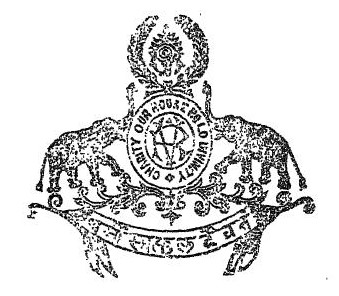
\includegraphics{fig.4.jpeg}

\hspace{0.5cm}\huge{\textbf{आर्यभटीयम्~~~~।}}\\

\vspace{.2cm}
\large{(द्वितीयो भागः)}\\
\rule{2cm}{.5mm} 

 \vspace{0.2cm}
%\hfill\break

\huge{\textbf{\en ĀRYABHAṬĪYA}}\\

\vspace{0.2cm}

\Large{\en Part~II} \\

\rule{2cm}{.5mm} 

\vspace{0.2cm}

{\footnotesize\textbf{\en EDITED BY}}

\vspace{0.3cm} \textbf{\en K.~SĀMBAŚIVA ŚĀSTRĪ,}\\
\vspace{0.2cm}
\small\emph{\en Curator of the Department for the Publication of}

\emph{\en Oriental Manuscripts, Trivandrum.}

\rule{2cm}{.5mm} 

{\en PUBLISHED UNDER THE AUTHORITY OF THE GOVERNMENT OF \\HER HIGHNESS THE MAHARANI REGENT OF TRAVANCORE}

\rule{2cm}{.5mm} 

\vspace{0.3cm}\scriptsize{\textbf{\en TRIVANDRUM: PRINTED BY THE SUPERINTENDENT, GOVERNMENT PRESS, 1931.}}
\end{center}

\newpage

\begin{center}
\large{\en TRIVANDRUM SANSKRIT SERIES}
 \vspace{0.3cm}

{\en No.~CX.}\\
\vspace{0.3cm}{\en  Śrī Setu Lakṣmī Prasādamālā.}
\vspace{0.3cm}

{\en No.~XXII.}

\vspace{1.5cm} 
{\en THE}

\vspace{0.3cm}
{\LARGE{\en ĀRYABHAṬĪYA}}

\vspace{0.3cm} 

{\en OF} 

\vspace{0.3cm}
\textbf{\en ĀRYABHAṬĀCĀRYA}

\vspace{0.3cm} 

{\footnotesize{\en WITH THE \emph{\en BHĀṢYA} OF}

\vspace{0.2cm} \en NĪLAKAṆṬHA SOMASUTVAN}

\vspace{1.5cm}{\footnotesize\textbf{EDITED BY}}

\vspace{0.3cm}
\textbf{\en K.~SĀMBAŚIVA ŚĀSTRĪ,}\\
\vspace{0.2cm}
\emph{\en Curator of the Department for the Publication \\
of Oriental Manuscripts, Trivandrum.}\\
\rule{2cm}{0.3mm}\\
\vspace{0.4cm}
\rule{6cm}{0.3mm}\\
{\textbf{Part~II \textendash\ \emph{\en Kālakriyāpāda.}}}\\
\rule{6cm}{0.4mm}
\vspace{0.5cm}

\small{\en PUBLISHED UNDER THE AUTHORITY OF THE GOVERNMENT OF\\
HER HIGHNESS THE MAHARANI REGENT OF TRAVANCORE.}\\
\rule{2cm}{0.3mm}
\vspace{0.3cm}

\small{\en TRIVANDRUM:\\
PRINTED BY THE SUPERINTENDENT, GOVERNMENT PRESS,}

1931.
\end{center}

\emph{\en All Rights Reserved.}]\

\newpage

\begin{center}
\vspace{2cm}{\Large{\underline{\textbf{अनन्तशयनसंस्कृतग्रन्थावलिः~।}}}}

\vspace{0.4cm}\large\textbf{ग्रन्थाङ्कः~११०.}

\vspace{0.2cm}{\Large\textbf{श्रीसेतुलक्ष्मीप्रसादमाला }}

\vspace{0.2cm}\textbf{ग्रन्थाङ्कः~२२.}

\vspace{0.2cm}

{\Large\textbf{श्रीमदार्यभटाचार्यविरचितम् }}

\vspace{0.2cm}{\textbf{\huge\textbf{आर्यभटीयं }}}

\vspace{0.2cm}\textbf{गार्ग्यकेरलनीलकण्ठसोमसुत्वविरचित- }

\textbf{भाष्योपेतम्~।}

\vspace{0.2cm}

\textbf{पौरस्त्यग्रन्थप्रकाशनकार्याध्यक्षेण \\ के. साम्बशिवशास्त्रिणा\\ संशोधितम्~।}

\rule{2cm}{0.3mm}

\vspace{0.1cm}

\begin{center}
\rule{6cm}{0.3mm}\\
\vspace{0.2cm}
\textbf{द्वितीयः सम्पुटः \textendash\ कालक्रियापादः~। }\\
\rule{6cm}{0.3mm}
\end{center}

\vspace{0.1cm}

\textbf{तच्च \\ अनन्तशयने \\ महामहिमश्रीसेतुलक्ष्मीमहाराज्ञीशासनेन \\ राजकीयमुद्रणयन्त्रालये तदध्यक्षेण \\ मुद्रयित्वा प्रकाशितम्~।}

\rule{2cm}{0.3mm}

\vspace{3cm}{\textbf{कोलम्बाब्दाः ११०६. क्रैस्ताब्दाः १९३१. }}
\end{center}


\newpage

\pagestyle{empty}
%\begin{tikzpicture}
%[remember picture,overlay] \draw[line width=2pt] ($(current page.north %west)+(1in,-1in)$) rectangle ($(current page.south east)+(-1in,2in)$);
%\end{tikzpicture}

\begin{center}
\Large\textbf{॥~श्री~॥}\\
\textbf{श्रीपद्मनाभसेवि-\\न्यखिलश्रीवर्धनी महाराज्ञी~। \\ श्रीसेतुलक्ष्म्यभिख्या \\ प्रत्यक्षा जयति वञ्चिभूलक्ष्मीः~॥}

\vspace{.5cm}

\textbf{ग्रन्थावलिरियमिन्धे \\ प्रसाधिता तत्प्रसादगुणगुम्फा~।\\ श्रीसहितसेतुलक्ष्मी-\\ प्रसादमाला सुवर्णमणिचित्रा~॥}
\end{center}



\newpage
%\hfill\break

\begin{center}
\textbf{\en PREFACE}
\end{center}
{\en This is the second part of the \emph{Āryabhaṭīya}, the first part of which was published in this series with the \emph{Bhāṣya} of Gārgyakeralanīlakaṇṭhasomasutvan.\\

In consonance with the statement,} 

\begin{quote}
\textbf{आर्यभटस्त्रीणि गदति गणितं कालक्रियां गोलम्}
\end{quote}
\noindent {\en the topic dealt with here is} \textbf{कालक्रिया}. {\en This valuable commentary on the} \textbf{कालक्रियापाद} {\en composed of a few terse aphorisms renders invaluable service to the ancient science of astronomy with its citations of authority and illustrations, always bearing in mind the matter at hand and explaining with a wealth of cogent and many-sided reasoning. Wonderful are the methods of exposition of the author of this commentary who justifies his enunciations by exhaustive discussions, mentioning the manifold methods of ancient \emph{Ācāryas} in the process of making astronomical calculations. It is a matter for immnense gratification for Keraliyas that this commentary makes it palpably evident that the great Hindu \emph{Ācāryas} of the East like those of the West had recourse to independent mechanical contrivances for the purposes of accurate planetary observations and calculations.\\

We hope to dwell at length on the achievements of Nīlakaṇṭhasomayājin, the author of this commentary in the introduction to the \emph{Golapāda}, the third and final part of this work that is to be published shortly.\\

We are proud to mention that the two manuscripts that were utilized in the publication of this volume, belong to His Most Gracious Highness the Maharaja's Palace Library.}\\

\noindent{\emph{\en Trivandrum,}

\noindent$\emph{15-12-1106.}$}
\hspace{5cm} \textbf{\en K.~SĀMBAŚIVA ŚĀSTRĪ.}

\newpage
%\hfill\break

\begin{center}
\textbf{निवेदना}
\end{center}


%\hfill\break

द्वितीयोऽयं भागः सभाष्यस्यार्यभटीयस्य~। यत् पूर्वमितोऽधिकरणाद् गार्ग्यकेरलनीलकण्ठसोमसुत्वविरचितभाष्योपेतं प्रथमसम्पुटात्मना प्राकाशि~।

\begin{quote}
\textbf{आर्यभटस्त्रीणि गदति गणितं कालक्रियां गोलम्}
\end{quote}

\noindent इति प्रतिज्ञानुरोधेन कालक्रियानिरूपणमिह प्रस्तुतम्~। बहुमुखाभिरुपपत्तिभिः प्रपञ्चनीयमर्थं मनसिकृत्य लघुगुलिकात्मना निर्मितस्य
कतिपयसूत्रबद्धस्यास्य कालक्रियापादस्य सप्रमाणं सोदाहरणं च क्रियमाणं विवरणमसामान्यं कमप्यनुग्रहमाविष्करोति ज्योतिषलोकस्य~। विशिष्य च ग्रहपरीक्षणे प्राचामाचार्याणामुच्चावचा गतीरुपन्यस्य कूलङ्कषाभिश्चर्च्चाभिरात्मसिद्धान्तं साधूकुर्वतोऽस्य भाष्यकारस्य प्रपञ्चनपद्धतयोऽत्यन्तायाद्भुताय~। अन्यच्च \textendash पाश्चात्यवत् पारैस्त्या अपि हैन्दवीया आचार्यवर्याः स्वतन्त्रैर्यन्त्रैर्ग्रहगणितविज्ञानेषु सूक्ष्मेक्षिकाभाजनमभूवन्नित्यपि विशकलय्य विशदयदिदमनन्यसामान्यं भाष्यं केरलीयानामस्माकमभिमानाय मानाधिकाय सम्पद्यते । एवंरीत्या भूयस्तरां वर्णनीयमहिम्नोऽस्य नीलकण्ठसोमयाजिनो भाष्यकारस्य प्रागल्भ्यपूरणीः पङ्क्तीरन्तिमभागतया प्रचिकाशयिषितस्य गोलपादस्योपोद्धातावसरे प्रवेशयितुमुत्सहमानोऽस्मि~। सद्यो विरमामि~।\\

\noindent एतत्प्रकाशनोपयोगिन्यौ मातृके द्वे अपि अस्मन्महाराजग्रन्थशालीये एवेत्यपरोऽयमभिमानः~।

\hfill\break

\noindent \emph{अनन्तशयनम्,}\\
\noindent \emph{१५-१२-११०६.}\hspace{5.9cm}  \textbf{के.~साम्बशिवशास्त्री.}


\newpage
\thispagestyle{empty}

%%%%%%%%%%%%%%%%%%%%%%%%%%%%%%%%%%%%%%%%%%%%%%%%%%%%%%%%
\begin{center}
	\textbf{विषयानुक्रमणी} \\
\end{center} 
%	\rule{0.08\linewidth}{0.3pt}
%\renewcommand{\arraystretch}{1.25}
%\vspace{1cm} 

\begin{tabular}{llp{0.6cm}r}
\hspace{1cm} \textbf{विषयः} &&& \textbf{पृष्ठम्} \\
	&&&\\
मङ्गलाचरणम्  & ....&&  ४\\
कालविभागः & .... &&  १\\
कालविभागस्य क्षेत्रेऽतिदेशः  & ....&&  २\\
युगे द्वयोर्द्वयोर्ग्रहयोर्योगकालज्ञानोपायः  & ....&&  २\\
व्यतीपातसङ्ख्याज्ञानम्  & ....&&  ,,\\
ग्रहोच्चनीचपरिवर्ताः & ....&&  ३\\
बार्हस्पत्याब्दलक्षणम्  & ....&&  ४\\
सौरचान्द्रसावननाक्षत्रमानानि  & ....&&  ,,\\
अधिमासलक्षणम् & ....&&  ५\\
अवमलक्षणम् & ....&&  ,,\\
मानुषवर्षप्रमाणम् & ....&&  ६\\
पितृवत्सरप्रमाणम्  & ....&&  ,,\\
दिव्यवत्सरप्रमाणम्  & ....&&  ,,\\
ब्राह्मदिनप्रमाणम्  & ....&&  ,,\\
उत्सर्पिणीलक्षणम् & ....&&  ८\\
अपसर्पिणीलक्षणम् & ....&&  ,,\\
सुषमालक्षणम् & ....&&  ,,\\
दुष्षमालक्षणम्& ....&&  ,,\\
'उत्सर्पिणी युगार्ध'मित्यस्य सूत्रस्य\\ ज्योतिर्गतिविषयत्वेनार्थविचारः  & ....&&  ,,\\
सप्तानां वायुस्कन्धानां मध्ये आवहप्रवहयोर्लक्षणम्  & ....&&  ९ \\
आर्यभटीयग्रन्थप्रणयनकालस्तदानीमार्यभटस्य वयःप्रमाणं च & ....&&  १२ \\
ग्रन्थप्रणयनकालेऽयनचलनाभावः  & ....&&  १३\\
अयनचलनस्य वृद्धिह्रासप्रकारः & ....&&  ,,\\
अयनचलनस्य परीक्षणप्रकारः  & ....&&  ,,\\
प्रसक्तानुप्रसक्त्या ग्रहगतेः परीक्षणप्रकारः  & ....&&  १४\\
तत्र ग्रन्थान्तरवाक्यानां प्रमाणतयोपन्यासः & ....&&  ,,\\
औदयिकार्धरात्रिकभेदेनार्यभटीयस्य तन्त्रस्य द्वैविध्यम् & ....&&  १७\\
युगाद्यारम्भकालोऽभीष्टकालानुमानप्रकारश्च & ....&&  १८\\
ग्रहाणां गतेः साम्यम् & ....&&  १९\\
ग्रहाणां गतिभेददर्शने कारणम् & ....&&   ,,\\
ग्रहाणां कक्ष्याक्रमः & ....&&  ,,\\

\end{tabular}

\newpage
%\hfill\break
\begin{center}२\\\end{center}
\vspace{0.5cm}
\renewcommand{\arraystretch}{1.25}
\begin{tabular}{llp{0.6cm}r}
	\hspace{1cm} \textbf{विषयः} &&& \textbf{पृष्ठम्} \\
	&&&\\
भास्करोक्तरीत्या ग्रहकक्ष्यानयनं मध्यमानयनं च & ....&&  २१\\
तन्त्रान्तरोक्तानामार्यभटीयोक्तानां च बिम्बव्यासयोजनानां\\ तारतम्यविवेचनम् & ....&&  २२\\
ग्रहाणां कालहोराधिपत्यम्  & ....&&  २७\\
ग्रहाणां वाराधिपत्यम्  & ....&&  ,,\\
इष्टाहर्गणानयनम्  & ....&&  २८\\
सूर्यसिद्धान्तोक्तरीत्याहर्गणानयनम्  & ....&&  ३०\\
वारप्रवृत्तौ मतभेदाः  & ....&& ,,\\
स्फुटोपपत्तिप्रदर्शनार्थे कक्ष्यामण्डले ग्रहभ्रमणप्रकारप्रदर्शनम्   & ....&&  ३१\\
प्रतिमण्डलप्रमाणं तत्स्थानं च  & ....&&  ३२\\
उच्चनीचवृत्ते ग्रहभ्रमणप्रकारः   & ....&&  ,,\\
मन्दकर्णाविशेषक्रिया  & ....&&  ३५\\
मन्दस्फुटकर्मणि परिलेखनप्रकारः  & ....&&  ३६\\
उच्चनीचवृत्तस्थाननिर्णयः  & ....&&  ३७\\
मन्दशीघ्रस्फुटकर्मणोर्विस्तरेण प्रतिपादनम्  & ....&&  ३८\textendash ४६\\
अविशेषक्रियां विना सकृत् कर्णानयने प्रमाणानि  & ....&&  ४७\\
रवीन्द्वोः स्फुटान्मध्यमानयनम् & ....&&  ४८\textendash ५०\\
मन्दशीघ्रस्फुटकर्मणोर्युक्तिप्रतिपादनम्  & ....&&  ५१\textendash ५४\\
भुजाफलधनर्णोपपत्तिः  & ....&&  ५४\textendash ६१\\
स्फुटगत्यानयनम्   & ....&&  ६१\textendash ६४
\end{tabular}	


\vspace{8mm}
\begin{center} 
\rule{2cm}{.3mm} 
\end{center}

\newpage
%\hfill\break

%\addtolength{\oddsidemargin}{0.1in}
%	\addtolength{\evensidemargin}{0.1in}
%	\addtolength{\textwidth}{4in}

%	\addtolength{\topmargin}{-.875in}
%	\addtolength{\textheight}{4in}
	

\begin{center}
\textbf{\vspace{2cm}{॥~श्रीः~॥}}

\textbf{\large श्रीमदार्यभटाचार्यविरचितम्}

\vspace{0.2cm}{\textbf{\LARGE आर्यभटीयं}}

\vspace{0.2cm}\textbf{\large गार्ग्यकेरलनीलकण्ठसोमसुत्वविरचितेन}

\vspace{0.2cm}\textbf{\large भाष्येण समेतम्~।}

\rule{3cm}{.3mm} 

\vspace{0.2cm}
(द्वितीयो भागः~।)

\vspace{0.2cm}
\textbf{अथ कालक्रियापादः~।}\\
%\rule{5cm}{0.2mm}\\
\vspace{0.4cm}
\textbf{अनादिनिधनं कालं तल्लिङ्गग्रहतारकाः~।\\
नत्वा भुवं च सर्वत्रेहानुमा तस्य दर्श्यते~॥}
\end{center}

यच्छेषतयात्र लौकिकगणितन्यायमशेषं गणितपादेन प्रत्य\renewcommand{\thefootnote}{१}\footnote{'त्यवद' क. पाठः}पीपदत्, तमेव कालं ज्योतिर्गतिविशेषैरनुमापयितुं कालक्रियापाद आरभ्यते~। तत्र मन्त्रार्थवादेतिहासपुराणेषु लोके च प्रसिद्धः कालविभाग एव क्षेत्रविभागेऽपि मूलं निरूप्यमाणे, इति प्रसिद्धस्तद्विभाग एव क्षेत्रेऽतिदिश्यते वर्षमित्यादिनार्याद्वितयेन\textendash

\begin{quote} 
{\ab वर्षं द्वादश मासास्त्रिंशद्दिवसो भवेत् स मासस्तु~।\\
षष्टिर्नाड्यो दिवसः षष्टिश्च}\renewcommand{\thefootnote}{*}\footnote{'षष्टिस्तु' इति मुद्रितपाठः.} 
{\ab विनाडिका नाडी~॥~१~॥\\
गुर्वक्षराणि षष्टिर्विनाडिकार्क्षी षडेव वा प्राणाः~।\\
एवं कालविभागः क्षेत्रविभागस्तथा भगणात्~॥~२~॥}
\end{quote}

इति~। यथा वर्षं (स्या ? स्वा)वयवभूतैर्द्वादशभिर्मासैरारब्धं स मासः पुनर्न तथा तावतिथैरंशैरारब्धः, स्वावयवभूतैर्दिवसैस्त्रिंशतैवारब्धः~।
अतस्त्रिंशांशा एव स्वावयवा दिवसा इत्युभयत्रावयवावयविसम्बन्धगतो भेदस्तु शब्देन द्योत्यते~। षष्टिर्नाड्यो दिवस इत्यत्रापि तुशब्दोऽनुवर्तनी(च?
यः), अस्यापि पूर्वस्माद् भिन्नत्वात्~। षष्टिश्च विनाडिका नाडीत्यत्र च शब्देनातः परं विभागसाम्यं द्योत्यते~। एष विभागः सौरादिषु मानेषु सर्वत्र समानः~।

\afterpage{\fancyhead[CE] {आर्यभटीये सभाष्ये }}
\afterpage{\fancyhead[CO]{कालक्रियापादः~। }}
\afterpage{\fancyhead[LE,RO]{\thepage}}
\cfoot{}

\newpage
%%%%%%%%%%%%%%%%%%%%%%%%%%%%%%%%%%%%%%%%%%%%%%%%%%%%%%%%%%%%%%
\renewcommand{\thepage}{\devanagarinumeral{page}}
\setcounter{page}{2}

%{\scriptsize\textbf {2. P. T. 1838. 500 12-4-1106. B}}

%\newpage
%\hfill\break
\vspace{3cm} २  \hspace{4cm}  आर्यभटीये सभाष्ये

\vspace{0.3cm} 
\noindent किन्तु गुर्वक्षराणि षष्टिरार्क्षी विनाडिका, आर्क्ष्या विनाड्याः षष्ट्यंश एव मध्यमवृत्त्या गुर्वक्षरोच्चारणकालः~। स्वस्थस्य जन्तोर्निःश्वासश्च तस्या एव षडंशः~। {\qt प्राणेनैति कलां भं} इतत्यस्य विवरणमेतत्~। समानान्तरगतानां विनाडीनां षष्ट्यंशा गुर्वक्षरान्महान्तोऽल्पाश्च स्युः~। एवं मुहुरपि षष्ट्यं\renewcommand{\thefootnote}{१}\footnote{'षष्ट्यः प्रा'}शा एव 
तदवयवा (एव~। ?) ग्राह्याः~। एतस्य विभागस्य त्रिरावृत्तत्वात् पुनरन्यादृशस्याप्रसिद्धत्वाच्चेति भावः~। एवं यः कालविभागः प्रसिद्धः
वर्षादिगुर्वक्षरान्तः, भगणात् प्रभृति तदवयव\renewcommand{\thefootnote}{२}\footnote{'वानां \ldots \ldots त'}भूतानां राश्यादीनां तत्परान्तानां विभागोऽप्येवमेवेति कालविभागस्य क्षेत्रेऽतिदेशोऽत्र क्रियत इति~॥ १\textendash२ ॥ \\

द्वयोर्द्वयोर्ग्रहयोर्यावन्त एकस्मिन् युगे योगास्ते\renewcommand{\thefootnote}{३}\footnote{'स्ते वि'}ऽपि विज्ञेया
एव, यतस्तयोरन्तरकालो ज्ञातव्यः~। गुरुशनैश्चराद्ययोरभीष्टयोर्यदाकदाचिद्योगो दृष्टः, ततः कियति काले पुनस्तयोरेव ततो द्वितीयो योगो भविष्यतीत्यादिज्ञाने ताभिर्यागावृत्तिभिः तदन्तरालकालस्य ज्ञेयत्वात्ता अपि ज्ञेयाः~। ताश्च गीतिकापटितैस्तयोर्भगणैरेव ज्ञेया इति
तत्प्रदर्शनार्थम् आर्यार्धमाह\textendash

\begin{quote}
{\ab भगणा द्वयोर्द्वयोर्ये विशेषशेषा युगे द्वियोगास्ते~।}
\end{quote}

इति~। विशेषशेषा (ये) द्वयोर्द्वयोर्भगणयोस्त एव युगे द्वियोगाः द्वयोर्बिम्बयोगसङ्ख्येति~। न केवलं ग्रहाणामेव योगसङ्ख्या ज्ञेयाः,
उच्चग्रहयोगसङ्ख्याः पातग्रहयोगसङ्ख्याश्च ज्ञेयाः~। तत्तत्स्फुटगत्यावृत्ति\renewcommand{\thefootnote}{४}\footnote{'त'}कालज्ञानार्थं च ग्रहोच्चयोगज्ञानं, विक्षेपप(र्यो ? र्य)यकालज्ञानार्थं ग्रहपातयोगाश्चेति द्वयो र्द्वयोर्योगे\renewcommand{\thefootnote}{५}\footnote{`ग एवेत्युक्तम्~।'} इत्येवोक्तम्~। येषामिह भगणाः प्रदर्शितास्तेषु
ययोर्योगा\renewcommand{\thefootnote}{६}\footnote{'योर्ययोर्यो' क. पाठः} जिज्ञास्यन्ते
तयोर्भगणविश्लेष एव तदा कर्तव्यः । तद्विश्लेषणे यः शेषः स एव तयोर्युगसम्बन्धिनी योगसङ्ख्येत्यर्थः~॥

एवं तिथ्यादिपर्ययस्य मासादि(क? का)लात्मकस्य प्रदर्शने विष्कम्भादियोगस्यापि प्रसङ्गात् तत्पर्ययांस्तद्गतव्यतीपातपर्ययांश्च
प्रदर्शयत्यूर्ध्वार्धेन\textendash

\begin{quote} 
{\ab रविशशिनक्षत्रगणाः सम्मिश्राश्च व्यतीपाताः~॥~३~॥}
\end{quote}
इति~। रविशशिनक्षत्रगणाः सम्मिश्रा व्यतीपाताः~। रविशशिनक्षत्रगणयोगा इत्युच्यमाने अनन्तरप्रदर्शितबिम्बयोगा एव प्रतीयेरन्~। अतस्तद्व्युदासार्थं संमिश्रग्रहणम्~। संमिश्रा रविशशिनक्षत्रगणाः सम्यङ् मिश्रो येषां ते संमिश्राः तयोर्भगणयोः सङ्ख्यासम्मिश्रणे व्यतीपातसङ्ख्या
ज्ञेयेत्यर्थः~।
 
\newpage
%\hfill\break

%\vspace{3cm} 
\hspace{4cm}कालक्रियापादः~। \hspace{4cm}३

\vspace{0.3cm} \noindent इति विष्कम्भादियोगप(र्या ? र्य)याः प्रदर्शिताः~। व्यतीपातानां प्रत्येकं
तावत्यः सङ्ख्या गतिश्च तेनैव सिद्धाः यत एकस्मिंश्चन्द्रार्कयोगपर्ययेऽत्र त्रयो
व्यतीपाताः चक्रव्यतीपातश्चक्रार्धव्यतीपातः सार्पमस्तकश्च~। भास्करश्चाह\textendash

\begin{quote}
{\qt सूर्येन्दुयोगे चक्रार्धे व्यतीपातोऽथ वैधृतः~।\\
चक्रे च मैत्रपर्यन्ते विज्ञेयः सार्पमस्तकः~॥}
\end{quote}

\noindent सूर्यसिद्धान्तेऽपि त्रिसङ्ख्यत्वमुक्तं व्यतीपातानां,

\begin{quote} 
{\qt व्यतीपातत्रयं घोरं गण्डान्तत्रितयं तथा~।} 
\end{quote} 
इति\renewcommand{\thefootnote}{१}\footnote{'ति~। पु'}। यः पुनरिह प्रासङ्गिकतया प्राप्तावसरः चन्द्रार्कयोगः स
चैवंभूत इति तत्सङ्गतिश्चकारेण सूच्यते~॥ ३ ॥ \\

तत्र तिथिकरणयोर्ज्ञाने\renewcommand{\thefootnote}{२}\footnote{'ने चन्द्रा} योगज्ञाने च चन्द्रार्कौ स्फुटीकृत्यैव
तद्विश्लेषो योगो वा कार्य इति, तद्भगणैर्न त्रैराशिकेन मध्यमानयनं कार्यमिति, ग्रहभगणविश्लेषयोगयोः कुट्टाकार एवोपयोगः~। तत्कुट्टाकारस्य च ग्रहगतिपरीक्षायां जातके चोपयोग इति तयोर्नात्र प्राचुर्येण व्यवहारः~। ग्रहोच्चभगणान्तरेणेह प्राचुर्येण स्फुटकर्मण्युपयोगात् तन्मध्यमानयनं च सार्वकालीनमेवेत्यत आह\textendash

\begin{quote}
{\ab स्वोच्चभगणाः स्वभगणैर्विशेषिताः स्वोच्चनीचपरिवर्ताः~।}
\end{quote}

\noindent इति~। स्वोच्चभगणाः स्वभगणैर्विशेषिताः स्वभगणेभ्यो मन्दोच्चभगणान् विशोध्य शीघ्रोच्चभगणेभ्यः स्वभगणांश्च विशोध्य ये ये शिष्टा लब्धास्ते ते स्वोच्चनीचपरिवर्ताः~। स्वस्य स्वस्य प्रतियुगं मन्दोच्चनीचवृत्ते\renewcommand{\thefootnote}{३}\footnote{'ते' च ता' क. पाठः} शीघ्रोच्चनीचवृत्ते च तावन्तः परिवर्ताः स्युः~। ततस्तैर्ग्रहवन्मध्यमानयनमपि
कार्यमित्यभिप्रायः~। वक्ष्यति च\textendash 

\begin{quote}
{\qt वृत्तपरिधौ ग्रहास्ते मध्यमचारं भ्रमन्त्येव~।}
\end{quote} 

\noindent इति~। तत्र यो मध्यमचारत्वेन विवक्षितः स एतैरहर्गणेन च त्रैराशिकेनानेय इति~। द्वियोगन्यायेन सिद्धेऽपि विविच्य ग्रहणाय पुनरपि तदुक्तिरित्यस्य स्वोच्चनीचवृत्तगतिप्रदर्शनपरत्वात् न पौनरुक्त्यमिति~।

\newpage
%\hfill\break

\vspace{3cm}४ \hspace{4cm} आर्यभटीये सभाष्ये

\vspace{0.3cm}
\begin{sloppypar} 
प्रदर्शितैर्भगणैर्मानविशेषान् प्रदर्शयन् बार्हस्पत्यस्य मानस्य
संवत्सरात्मक\renewcommand{\thefootnote}{१}\footnote{'त्वा(द)स्या' ख. पाठः}त्वस्यापि 
बृहस्पतिराशिचारात्मकत्वात् तदधिष्ठितप्रदेशवशाज्जायमानानां तद्विशेषाणां तत्तदनुरूपसं ज्ञाविशेषसम्भवाच्च तद्द्वादशसंवत्सरात्मकतत्पर्ययो\renewcommand{\thefootnote}{२}\footnote{'र्या'} यः, यच्च
पञ्चसंवत्सरात्मकं युगं संवत्सरपरिवत्सरेडावत्सरानुवत्सरवत्सराख्यं, तयोरुभयोर्यदा युगपत्समाप्तिरिति
निरूप्यमाणेऽब्दगणे षष्टिमिते तस्य परिसमाप्तिरवगम्यत इति प्रभवादिक्षयपर्यन्तः स षष्ट्यब्दगणो लोके प्रसिद्धः~। तद्द्वारा च गतकालविज्ञानम् इत्यहर्गणस्य तद्द्वारत्वात् प्रथमं बार्हस्पत्याब्दं प्रदर्शयति\textendash
\end{sloppypar} 

\begin{quote}
{\ab गुरुभगणा राशिगुणास्त्वाश्वयुजाद्या गुरोरब्दाः~॥~४~॥}
\end{quote}

%\hfill\break

इति~। गुरुभगणा राशिगुणा गुरोरब्दा युगसम्बन्धिनो बार्हस्पत्याब्दाः\renewcommand{\thefootnote}{३}\footnote{'ब्द' क, पाठः} (स्य~? स्युः)~। ततस्त्रैराशिकाद् वर्तमानबार्हस्पत्याब्दो विज्ञेयः~।
ततस्तदर्थं तन्मध्यमे तदतीतभगणा राशिगुणाः क्षेप्याः~। ततो वर्तमानसंवत्सरश्च ज्ञेयः~। ते चाश्वयुजाद्याः~। उक्तं च सूर्यसिद्धान्ते तदानयनं\textendash

\begin{quote}
{\qt द्वादशघ्ना गुरोर्याता\renewcommand{\thefootnote}{४}\footnote{'त' ख. पाठः} भगणा वर्तमानकैः~।\\
राशिभिः सहिताः शुद्धाः षष्ट्या स्युर्विजयादयः~॥}
\end{quote}
 ॥~इति~॥ ४ ॥\\

पुनरपि मानुषाण्येव मानान्याह\textendash

%\hfill\break
\begin{quote} 
{\ab रविभगणा रव्यब्दा रविशशियोगा भवन्ति शशिमासाः~।\\
रविभूयोगा दिवसा भावर्ताश्चापि नाक्षत्राः~॥~५~॥}
\end{quote} 

%\hfill\break

\noindent इति~। रविभगणा रव्यब्दाः~। मेषादिमीनान्तैर्द्वादशभिर्मासैरारब्धा रविभगणाः~। भगणानां\renewcommand{\thefootnote}{५}\footnote{भग्रहाणां मे' क. पाठः} मेषादित्वं च {\qt बुधाह्न्यजार्कोदयाच्च लङ्कायां} इत्युक्तम्~। रविशशियोगाः शशिमासा भवन्ति~। न पुना रविशशिभगणयोगाः~। तयोर्बिम्बयोगान्त एको मासः~। विप्रकर्षसन्निकर्षौ चार्धमासौ~। रविभूयोगा दिवसाः~। अत्रापि बिम्बयोगा\renewcommand{\thefootnote}{६}\footnote{'ग' ख, पाठः} एव~। तस्माद् रविभूभगणानां वियोगा दिवसाः~। उक्ताश्च रविशशिभुवां भगणाः\textendash

\begin{quote} 
{\qt युगरविभगणाः ख्युघृ शशि चयगियिङुशुछ्ऌ कुङिशि बुण्लृख्षृ प्राक्~।}
\end{quote}

\newpage
%\hfill\break

\vspace{3cm} \hspace{4cm}कालक्रियापादः~। \hspace{4cm}५

\vspace{0.3cm}
\noindent इति~। द्रष्ट्रपेक्षयैकसूत्रगतत्व (ए)व द्वयोर्द्वयोर्योगश्च विवक्षितः~।
न पुनर्द्वयोद्वयोर्ग्रहयोर्बिम्बयोगः सम्भवति, कक्ष्याभेदस्य वक्ष्यमाणत्वात्~।
तदुक्तं सूर्यसिद्धान्ते\renewcommand{\thefootnote}{१}\footnote{'न्ते\dots ' क. पाठः}ऽपि\textendash 

\begin{quote}
{\qt भावाभावाय लोकानां कल्पनेयं प्रदर्शिता~।\\
स्वमार्गगाः प्रयान्त्येते दूरमन्योन्यमाश्रिताः~॥}
\end{quote}

\noindent इति~। अतो रविभूभगणान्तरतुल्या एव दिवसाः~। दिवसशब्देनैषां सावनत्वमपि सिद्धं, यतः सावन एव दिवसशब्दो मुख्यतया वर्तते~। लक्षणयैवार्क\renewcommand{\thefootnote}{२}\footnote{'र्क्ष' ख. पाठः}चन्द्रादिषु~। भावर्ताश्चापि नाक्षत्राः~। दिवसा इत्यनुवर्तते~। भानामश्विन्यादीनामा\renewcommand{\thefootnote}{३}\footnote{'नां ना'}वर्तः प्रत्यग्भ्रमणं नाक्षत्रो दिवसः~। भूभगणा एव नाक्षत्रा दिवसा इति यावत्~। यद्वा अश्विन्यादीनां पौष्णान्तानां नक्षत्राणां परिवर्तो नाक्षत्रः\renewcommand{\thefootnote}{४}\footnote{'त्रस'}~। नक्षत्रसम्बन्धी मास इति चार्थात् सिध्यति~।
लक्षणयैव हि माना\renewcommand{\thefootnote}{५}\footnote{दिषु' क. पाठः}न्तरेषु मासादिशब्दा वर्तन्ते~। तत्र मासशब्दश्चान्द्र एव मुख्यतया वर्तते~। 

\begin{quote}
{\qt इन्द्राग्नी यत्र हूयेते मासादिः स प्रकीर्तितः~।\\
अग्नीषोमौ स्थितौ मध्ये समाप्तौ पितृसोमकौ~॥}
\end{quote}

\noindent इति हि मासलक्षणं वदन्ति सन्तः~। तत्र चन्द्रभगणस्य मासासन्नत्वात् मासेनैव च सम्बन्धः, न पुनर्दिवसादिना संवत्सरेण च~। तस्माच्चन्द्रभणस्य मासत्वमेव युक्तम्~। तस्मात् तत्रैव मासशब्दस्य लक्षणाव्यापारोऽपि युज्यते~। बार्हस्पत्यमाने बृहस्पतिचारोऽपि संवत्सर एव, तस्य संवत्सरासन्नत्वात्~। तथा चन्द्रभगणोऽपि मास एव~। तथा भानां प्रत्यग्भ्रमणमपि दिनमेव, तस्यापि रविप्रत्यग्भ्रमणासन्नत्वादेव~॥ ५ ॥\\

अत्रोक्तैः सौरचान्द्रसावनात्मकैर्वर्षमासदिवसैरधिमासावमा(सा\renewcommand{\thefootnote}{६}\footnote{'दाभ्यां' ख. पाठः}?)भ्यां चाहर्गण आनीयत इति तावप्याह\textendash

\begin{quote}
{\ab अधिमासका युगे ते रविमासेभ्योऽधिकास्तु ये चान्द्राः~।\\
शशिदिवसा विज्ञेया भूदिवसोनास्तिथिप्रलयाः~॥~६~॥}
\end{quote}

\newpage

%\hfill\break
\vspace{3cm}६ \hspace{4cm} आर्यभटीये सभाष्ये

\vspace{0.3cm}
\noindent इति~। त्रयोदशहतरविभग(णैः?णेभ्यः) क(लि?ल्प)चन्द्रभगणानां यावद्भिराधिक्यं तावन्त एव युगेऽधिमासा इत्युक्तं भवति, यतश्चन्द्रभगणात् केवलरविभगणं विशोध्य चान्द्रमासा लभ्यन्ते~। तेभ्योऽपि पुनर्द्वादशहतान् रविभगणान् विशोध्याधिमासाश्च लभ्यन्ते, यतः प्रत्यब्दं ये त्रयोदशशशिभगणातिरिक्ताश्चन्द्रभुक्तभागाः तेषु द्वादशहृतेषु अधिकतिथयश्च लभ्यन्ते~। अतः प्रत्यब्दमेकादशाधिकतिथयः सावयवाः स्युः~। कुतस्तेषां द्वादशहरणात् तत्सिद्धिः~।

\begin{quote}
{\qt अर्काद्विनिस्सृतः प्राचीं यद् यात्यहरहः शशी~।\\
    तच्चान्द्रमानमंशैस्तु ज्ञेया द्वादशभिस्तिथिः~॥}
\end{quote}

\noindent इति वचनादादित्यात् प्राग्गतानां चन्द्रभुक्तभागानां द्वादशभिर्हरणेन\renewcommand{\thefootnote}{१}\footnote{'णे ति' ख. पाठः} तिथि सिद्धेः~। चान्द्रमासानां सौरमासेभ्यः सङ्ख्ययाधिक्यादेव परिमाणतोऽल्पत्वमपि सिद्धम्~। यतोऽल्पेन मीयमानं वस्तु धान्यादिकं महता मानेन मीयमानात् सङ्ख्ययातिरिच्यते, एवं महता सावनदिवसेन मीयमानाद् युगात् ततोऽल्पेन चान्द्रदिवसेन मीयमानं युगमतिरिच्यत इति युगसावनाद् युगचान्द्रदिवसानां सङ्ख्ययाधिक्यम्~। तावतीनां तिथीनां सावनेषु प्रलीनत्वात् सावनेभ्योऽति\renewcommand{\thefootnote}{२}\footnote{नेऽप्यति' क. पाठः}रिक्तानां चान्द्रदिनानां तिथिप्रलयोक्तिर्युज्यते~॥ ६ ॥ \\

एवं मानुषाणि षण्मानानि प्रतिपाद्य पित्र्यदिव्यप्राजापत्यानां मानानां स्वरूपं दर्शयति\textendash 

\begin{quote}
 {\ab रविवर्षं मानुष्यं तदपि त्रिंशद्गुणं भवति पित्र्यम्~।\\
पित्र्यं द्वादशगुणितं दिव्यं वर्षे समुद्दिष्टम्~॥~७~॥

दिव्यं वर्षसहस्रं ग्रहसामान्यं युगं द्विषट्कगुणम्~।\\
अष्टोत्तरं सहस्रं ब्राह्मो दिवसो ग्रहयुगानाम्~॥~८~॥}
\end{quote}

इति~। रविवर्षं मानुष्यमित्यनुवादेन संवत्सरशब्दस्य रविवर्ष एव मुख्यतया वृत्तिः, अन्यत्र तु लक्षणयेति द्योत्यते~। तदपि त्रिंशद्गुणं
भवति पित्र्यमिति पितॄणां शशिमण्डलगतत्वादमावास्यायां च शशिनः समोपरिष्टात् सूर्यावस्थितेस्तदैव तेषां मध्याह्नः~। अत एवापरपक्षमध्ये चोदय
इत्यपरपक्षो-
\newpage

%\hfill\break
\vspace{3cm} \hspace{4cm} कालक्रियापादः~। \hspace{4cm} ७

\vspace{0.3cm}

\noindent त्तरार्धं पूर्वपक्षाद्यार्धं च तेषां दिवसः~। पूर्वपक्षान्त्यार्धमपरपक्षाद्यार्धं च रात्रिः~। अतश्चान्द्रमासोऽहोरात्रः~। मासाश्च प्रत्यब्दं द्वादश~। अतः संवत्सराणां त्रिंशति षष्ट्युत्तरशतत्रयसङ्ख्यास्तेषाम् अहोरात्राः~। अतो मानुष्यैस्त्रिंशताब्दैः तेषामेकं वर्षं स्यात्~। पित्र्यं वर्षं द्वादशगुणितं दिव्यं वर्षं स्यात्~। एवं सति मानुष्यैः षष्ट्युत्तरशतत्रयसङ्ख्यैः दिव्यं वर्षं स्यादिति सिद्धं भवति~। ननु सौरमासस्यैव हि पित्र्यदिनत्वमत्रोक्तं, तदपीत्यत्र तच्छब्देन प्रकृतस्य सौरस्यैव परामर्शो युज्यत इति चेत्~। नैष दोषः~। {\qt रविवर्षार्धं मनुजाः} इति चान्द्रमासस्यैव पित्र्यदिनत्वेन वक्ष्यमाणत्वात् स एव पितॄणामहोरात्रः, न सौर इति निश्चीयते~। शशिगा इति विशेषणं च हेतुगर्भं शशिगत्वादित्यर्थः~। तस्माच्चान्द्राणामेव पित्र्यदिन(त्त्वे?त्वं)न सौराणाम्~। तर्हि {\qt पित्र्यं द्वादशगुणितं दिव्यं वर्षम्} इत्यत्रापि पित्र्याब्दानामेव
द्वादशगुणितानां दिव्यवर्षत्वं\renewcommand{\thefootnote}{१}\footnote{'त्वमुक्तं यु' क. पाठः} युक्तम्~। तथा सति चन्द्राब्दैरेव षष्ट्युत्तरशतत्रयसङ्ख्यैरेकं दिव्यं वर्षं स्यात् न सौरैरिति चेत्~। तच्च न युक्तम्~। {\qt रविवर्षार्धं देवाः पश्यन्त्युदितं रविम्}\renewcommand{\thefootnote}{२}\footnote{'मिति व' ख. पाठः} इत्यादि वक्ष्यमाणत्वादिति~। तदनुगुणतयैव {\qt तदपि त्रिंशद्गुणं भवति पित्र्यम्} इत्युक्तम्\renewcommand{\thefootnote}{३}\footnote{'त्र्यमुक्त'}~। तेन प्राप्तं
पित्र्यदिनस्य सौरत्वं गोलपादे निराकरिष्यते च~। तस्मात् प्रायिकत्वमेव{\qt तदपि त्रिशद्गुणं भवति पित्र्यम्} इत्यस्य\renewcommand{\thefootnote}{४}\footnote{'स्य प्रा'}~। तस्य प्रायिकतयोक्तिश्व दिव्यवर्षस्य
प्राधान्येन प्रतिपाद्यत्वात् तदानुगु\renewcommand{\thefootnote}{५}\footnote{'दनुगुणैः दि}(ण्योश्चै ? ण्याच्चै) वेति न कश्चिद्
दोषः~। {\qt दिव्यं वर्षसहस्रं ग्रहसामान्यं युगं द्विषट्कगुणम्} इत्यत्र युगस्य ग्रहसामान्यमित्येतद्विशेषणं द्व्यादिग्रहयुगव्यावृत्त्यर्थम्~। यत्र द्वयोर्ग्रहयोरपि युगपद् भगणपरिपूर्तिः स्यात् तत् तयोरेव युगम्~। एवं द्वयोर्द्वयोर्ग्रहयोः पृथक् पृथग् युगं भिद्यते~। अत एव सूर्यसिद्धान्तेऽपि\textendash

\begin{quote} 
{\qt चतुर्विंशो युगस्यांशः सूर्याचन्द्रमसोर्युगम्~।}
\end{quote} 

इत्युक्तम्~। तस्मात् सर्वेषां साधारणं युगं यत् तद् द्विषट्कगुणं दिव्यं वर्षसहस्रम्~। द्विषट्कगुणमित्यनेन तस्यार्धयोर्वैधर्म्यं द्योत्यते~।
{\qt अष्टोत्तरं सहस्रं ब्राह्मो दिवसो ग्रहयुगानाम्} इत्यनेन ब्राह्ममानं प्रदर्श्यते~। तत्र दिवस शब्देनाहरेर्वोच्यते\renewcommand{\thefootnote}{६}\footnote{'ते ता' क. पाठः} नाहोरात्रः~। तेन तावती रात्रिश्च~। तैरहोरात्रैः षष्ट्युत्तरै-

\newpage

%\hfill\break

\vspace{3cm} ८ \hspace{4cm}आर्यभटीये सभाष्ये

\vspace{0.3cm}
\begin{sloppypar} 
\noindent स्त्रिभिः शतैस्तस्याप्येकं वर्षम्~। तेषां शतं तस्यायुः~। प्रलयकालश्च तावान् इत्येतच्चात्रैव सूचितम्~। तत्र तस्य गतैर्वर्षै र्दिवसैर्वा न ग्रहगणित उपयोगः,कल्पादिगतकालेनैव ग्रहगतिरनुमीयते~। तस्य रात्रौ ग्रहाणामभावाद् इति तद्गतदिनादिकं न प्रदर्शितम्~। वर्तमानकल्पगतं तु पूर्वमेव प्रदर्शितम्~।
\end{sloppypar}

\begin{quote}   
{\qt काहोमनवो ढ मनुयुग श्ख गतास्ते च मनुयुग छ्ना च~।\\
कल्पादेर्युगपादा ग च गुरुदिवसाच्च भारतात् पूर्वम्~॥}
\end{quote}

\noindent इति~। अत्रापि {\qt काहोमनवो ढ मनुयुग श्ख} इत्यनेनाष्टोत्तरं सहस्रं ब्राह्मो दिवसो ग्रहयुगानामित्येतत् सिद्धं, यतो द्वासप्ततियुगं मन्वन्तरं, मनवश्चैकस्मिन्नहनि चतुर्दश इत्युक्ते चतुर्दशगुणिताया द्वासप्ततेरष्टोत्तरसह स्रत्वं सिद्धम्~। अतस्तेषामष्टोत्तरं सहस्रं ब्रह्मणो दिनमिति च सिद्धम् इति~। गतास्ते च ते मनवश्च षड् गताः~। मनुयुगानि छ्ना च गतानि~। (प्र?)वृत्तपूरणायात्र दीर्घप्रयोगः~। सप्तमस्य मनोः सप्तविंशतिर्युगानि च कल्पादेः प्रभृति गतानि~। वर्तमानचतुर्युगस्य पादा अपि त्रयो गताः~। तदा गुरुदिवसाद् भारतात् पूर्वमष्टाविंशे युगे द्वापरान्ते कल्पादेः प्रभृत्येतावान् कालो गत इत्यर्थः\renewcommand{\thefootnote}{१}\footnote{'र्थः~। चतुर्युगस्य पू' ख. पाठः}~॥ ७\textendash ८ ॥ \\

चतुर्युगस्यार्धशो यो भेदस्तमेवा(ह)\textendash

\begin{quote} 
{\ab उत्सर्पिणी युगार्धं पश्चादपसर्पिणी युगार्धं च~।\\
मध्ये युगस्य सुषमादावन्ते दुष्षमेन्दूच्चात्~॥~९~॥}
\end{quote}

इति~। अनेन कालकृता प्राणिनामवस्थोच्यते~। चतुर्युगस्य पूर्वार्धमुत्सर्पिणीकालः अपरार्धमपसर्पिणीकालः~। तिरश्चा मनुष्याणां च वीर्योत्कर्षो धर्मोत्कर्षश्च उत्सर्पिण्याख्यावस्था~। तदपकर्षोऽपसर्पिणी नाम~। जम्बूद्वीप एवैषा युगावस्था~। प्ल(वा ? क्षा)दिषु पुनस्त्रेतायुगसम एव कृत्स्नः
कालः~। नत्वेव तु युगावस्था तेषु~। तस्मादेतद्देशभवैवैषावस्था~। एषा युगावस्था श्रीविष्णुपुराणेऽप्युक्ता {\qt उत्सर्पिणी} इत्यादिना~। अथवा
ज्योतिर्गतिविषयमेवैतत् सूत्रम्~। तत्र युगशब्देन ग्रहसामान्ययुगं वा ययोः कयोर्युगं वा विवक्ष्यते~। तत्राद्यः पक्षो न युज्यते~। {\qt क्षितिरवियोगात्} इत्यादिना वक्ष्यमाणेन विरोधात्~। तत्र हि स्वग्रन्थकरणकाले दृक्साम्यं गीतिकोक्तभगणा-

\newpage
%\hfill\break

\vspace{3cm} \hspace{4cm}कालक्रियापादः~। \hspace{4cm}९ 

\vspace{0.3cm}
\noindent दीनां साधितम्~। तदा ग्रहसामान्ये युगे चतुर्थपादस्य वर्तमानत्वाद् ग्रहसामान्ययुगविवक्षायां दुष्षमत्वापत्तेः~। ये पुनर्गीतिकासु पठितानां गतिमतां द्वयोर्द्वयोर्युगाख्या योगाः मीनान्तभवाः, ते\renewcommand{\thefootnote}{१}\footnote{'ते च' क. पाठः} पञ्चचत्वारिंशद्भेदभिन्नाः~। तैर्भगणवियोगैस्तेषाम् अवान्तरयोगाश्च त्रैराशिकेनानेयाः~। तद्वशाच्चोत्सर्पिण्यपसर्पिण्या अवस्थे स्तः~। कस्य पुनः सावस्था~। सा ज्योतिःसम्बन्धिन्येवेति प्रकरणादवगम्यते~। ज्योतिषां गतिर्ह्यत्र प्रकृता~। तत्र चाविशेषेणोक्तत्वात् कृत्स्नस्यैव भगोलस्य~। तस्येन्दूच्चादित्येकोऽवधिः~। अवव्यन्तरं पुनः किम्~। इन्दूच्चादित्यभिविधौ चेयं पञ्चमी~। इन्दूच्चप्राप्त्यन्तरा उत्सर्पिणी तत्प्राप्त्यनन्तरमपसर्पिणी\renewcommand{\thefootnote}{२}\footnote{'णीति त' ख. पाठः}~। (उत्सर्पिणी) कस्य
पुनरिन्दूच्चमपसर्पिणी कस्य पुनरिन्दूच्चम्~। सन्निकर्षविप्रकर्षयोर्भगोलस्योत्सर्पिण्यपसर्पिण्यौ~। सूर्ये \ldots \ldots\ त्कर्षः~। \ldots \ldots\ उच्चप्राप्तेः प्रभृति नीचयोगान्तमपकर्षः~। भुवमपेक्ष्य सन्निकर्षो विप्रकर्षश्च विवक्षितौ~। यतो भूमध्यमधऊर्ध्वदिशोरवधिः ततो भूमध्यात् प्रभृत्येवोर्ध्वगमनं युक्तम्, ऊर्ध्वदिशस्तत एव प्रवृत्तेः~। तद(न)न्तरमधोगमनमपि युक्तम्, इत्येतन्माधवोक्तेश्च सिद्धम्~। सदैव प्रवहान्तर्गर्भभूतावहवायुस्कन्धमध्यगतैव भूः~। तस्माद्वायुस्कन्धस्य भगोलस्य च प्रकृत्यैकत्रैव घनमध्यम्~। तस्यैवम्भूतो विकारोऽस्ति, (अथ) वा गोलमध्यापेक्षया भगोलमध्यस्य~। एवं परस्परसन्निकर्षविप्रकर्षात्
सर्वेषामप्यवयवानां संयोगवियोगौ\renewcommand{\thefootnote}{३}\footnote{'गौ~। त'} स्तः~। तस्मात् तयोः कतरस्यचिच्चलनम्~। एवं भगोलस्य वा वायुगोलस्य वा~। तच्च भगोलस्यैव युज्यते, धरित्र्या ब्रह्माण्डकटाहमध्यवर्तित्वोक्तेः, आवहस्य च विश्वम्भरया विशेष्यमाणत्वात्~। {\qt विश्वम्भरापवनमावहमाहुरेके} आव\renewcommand{\thefootnote}{४}\footnote{'ह \ldots \ldots\ र्थिकार्थ' क. पाठः}हश(का ? ब्दा)र्थनिरूपणेऽपि तन्मध्यगतत्वं सिद्धं विश्वम्भरायाः~। अवागावहतीत्यावह उच्यते~। अवाग्दिशोऽवधिश्च विश्वम्भरैव~। अतो विश्वम्भरा स्वेनैव वायुना तेन समन्ततो वस्तूनि सर्वाणि (अवाङ्)मुखमावहति~। अत आवहवायुः विश्वम्भरावायुरिति च संज्ञाद्वयमुपपद्यते~। तदूर्ध्वगतः प्रवहस्तु समन्तत एव वस्तूनि वहति~। सर्वाणि वस्तूनि भ्रामयन्नेव वहति इति प्रवहस्कन्धगतानां वस्तूनां भ्रमः, कदाचिदपि (न) विश्रान्तिरिति तद्वहनस्य प्रकर्षात् प्रवहशब्दवाच्यत्वम्~।

\newpage
%\hfill\break

\vspace{3cm} १०\hspace{4cm} आर्यभटीये सभाष्ये

\vspace{0.3cm}
\noindent वायुस्कन्धानां सप्तानामितरेतरसंश्लिष्टत्वात् सप्तभिर्वायुस्कन्धैर्व्याप्त एव ब्रह्माण्डकटाहान्तर्गताकाशः कृत्स्नोऽपि~। यद्यन्तरान्तरा यत्किञ्चिद् विवरं स्यात् तर्ह्येव तयोः कस्यचिच्चलनं\renewcommand{\thefootnote}{१}\footnote{'नं भ'} सम्भवति~। तच्च न युक्तं सदागतेः सर्व त्रैव व्याप्तेः~। तथा सति तत्स्कन्धानां सप्ता(न)तिरेकात् तदभावश्च
दर्शितः~। {\qt गि\renewcommand{\thefootnote}{२}\footnote{'हि'}यिङश कुवायुकक्ष्यान्त्य} इति कुवायुकक्ष्या
पञ्चसप्तत्यधिकशतत्रयोत्तरसहस्रत्रयसङ्ख्या~। कथं वायुकक्ष्याया ग्रहकक्ष्यावत् सङ्ख्योपदेशो\renewcommand{\thefootnote}{३}\footnote{'शा वा' क. पाठः} युज्य(ते) वायोः सर्वत्र व्याप्तत्वात्~। तन्मध्यपरिणाहस्य वा तत्पर्यन्तपरिणाहस्य वा अवान्तरप्रदेशस्य कस्यचिद् वेत्येतस्य संशयस्य निराकरणार्थम् अन्त्येत्युक्तम्~। प्रवहवायुसन्निकृष्टावयववा(न)यं परिणाहः~। किञ्च वायुगोलमध्यस्यभूमध्यस्य च विप्रकर्षे सति विषुवद्देशगतानामपि तद्वशात् तद्दर्शनादर्शनकालयोः क्रमेण न्यूनातिरेकौ सम्भवत इति चरव्यतिरेकेणापि दिनरा(त्र्योर्भे)दः स्यात्~। भूमेर्द्रष्ट्रभिमुखचलने दिनस्य न्यूनत्वं रात्रेराधिक्यं च~। यदा पुनर्द्रष्ट्रपेक्षयाधोगमनं भूमेस्तदा वैपरीत्येन च स्तः~। एवंभूतो विकारो न कदाचित् क्वापि केनचिदुपलभ्य(ते)~। ततः सदापि वायुस्कन्धमध्यगतैव भूरिति वायुस्कन्धात् तदपेक्षया भुवश्च न चलनं युक्तम्~। भगोलस्य तु वायुस्कन्धापेक्षयान्यादृशं चलनं प्रसिद्धमप्यस्त्येव~। 

\begin{quote}
{\qt त्रिंशत्कृत्वो युगे भांशैश्चक्रः प्राक् परिलम्बते~।}
\end{quote}

\noindent इत्यादिग्रन्थसन्दर्भेण तत्प्रकारस्य प्रदर्शितत्वात्~। 

\begin{quote} 
{\qt माघमासे धनिष्ठादिरुत्तरे(णे?णै)ति भानुमान्~।\\
प्रपद्येते श्रविष्ठादौ सूर्याचन्द्रमसावुदक्~॥\\
श्रविष्ठाद्यर्कतो वा स्यादुत्तरायणसंज्ञितः~।\\
कालः सा\renewcommand{\thefootnote}{४}\footnote{'स' ख. पाठः}र्पार्धपर्यन्तं याते भानावितीरितम्~॥}
\end{quote}

\noindent इत्यादिपरमर्षिवाक्यैरपि तच्चलनं सिद्धम्~। प्रभाकरश्चाह\textendash 

\begin{quote}
{\qt वसुदेवादिसार्पार्धादयनं मुनयो जगुः~।\\
मृगकर्क्यादितो दृष्टं कथं तद्धि गतैर्विना~॥}
\end{quote}

\noindent इति~। तत्र विप्रतिपन्नान् प्रति तत्समर्थनपरं वाक्यं वराहमिहिरोऽपि संहितायामाह\textendash 

\newpage
%\hfill\break

\vspace{3cm} \hspace{4cm}कालक्रियापादः~।\hspace{4cm} ११

\vspace{0.3cm}
\begin{quote}
{\qt आश्लेषार्धाद् दक्षिणमुत्तरमयनं रवेर्धनिष्ठाद्यम्~।\\
    नूनं कदाचिदासीद् येनोक्तं पूर्वशास्त्रेषु~॥\\
साम्प्रतमयनं सवितुः कर्कटकाद्यं मृगादितश्चान्यत्~।\\
उक्ता भांशैर्विकृतिः प्रत्यक्षपरीक्षणैर्व्यक्तिः~॥}
\end{quote}

\noindent इति~। तच्चलनपरिमाणस्य परीक्ष्य निर्णयस्तद्वशात् फलविशेषश्च उपरितनेन ग्रन्थेन प्रदर्शितः~। 

\begin{quote}
{\qt दूरस्थचिह्नवेधादुदयेऽस्त(मे ? मये)ऽपि वा सहस्रांशोः~।\\
छायाप्रवेशनिर्गमबिन्दोर्वा मण्डले महति~॥}
\end{quote}
\noindent इत्यादिना हि\renewcommand{\thefootnote}{१}\footnote{'ए' ख. पाठः} तच्चलनं प्रत्यक्षत उपलभ्यते तन्मूलैतिह्येन स्मृतेश्च~। तत्सर्वमुपरिष्टात् स्पष्टीकरिष्यामः~। तच्च तिर्यग्दिगनुसारेण~। एतत् पुनरूर्ध्वाधोदिगनुसारेण\renewcommand{\thefootnote}{२}\footnote{'ण~। त' क. पाठः}~। एतच्चलनवशाच्च दृग्गोलगतानां ग्रहाणां भेदः स्यात्, न च भगोलावयव\renewcommand{\thefootnote}{३}\footnote{'वविशेषसम्बन्धस्स'}सम्बन्धविशेषस्य~। इति तिथिनक्षत्रादिग्रहगतौ तस्योपयोगाभावात् तत्परिमाणं न प्रदर्शितम्~। तच्च लम्बनादि न्यायविदां परीक्ष्य
निर्णेतुं शक्यम्~। तन्न्यायाश्च गोलपादे प्रकाश्यन्ते~। तत्परिमाणं तन्मूलं गणितकर्म च ग्रहयोगाध्याये श्रीपतिराह\textendash

\begin{quote}
{\qt त्रिभविरहितचन्द्रोच्चोनभास्वद्भुजज्या\\
गगननृपविनिघ्नी भत्रयज्याविभक्ता\renewcommand{\thefootnote}{४}\footnote{'क्तं' ख. पाठः}।\\
भवति परफलाख्यं तत् पृथक्स्थं शरघ्नं\\
हृ\renewcommand{\thefootnote}{५}\footnote{'ह' क. पाठः}तमुडुपतिकर्णत्रिज्ययोरन्तरेण~॥\\
यदिह फलमवाप्तं तद्धनर्णं पृथक्स्थे\\
तुहिनकिरणक(र्णो ? णे) त्रिज्यकोनाधिकेऽथ~।\\
स्फुटदिनकरहीनादिन्दुतो या भुजज्या\\
स्फुटपरमफलघ्नी भाजिता त्रिज्ययाप्तम्~॥\\
शशिनि (च ? प)रफलाख्यं सूर्यहीनेन्दुगोलात्\\
तदृणमुत धनं स्यादुच्चहीनार्कगोलम्~।\\
यदि भवति हि याम्यं व्यस्तमेतद्विधेयं\\
स्फुटगणितदृगैक्यं कर्तुमिच्छद्भिरत्र~॥}
\end{quote}
  
\newpage
%\hfill\break

\vspace{3cm}
१२ \hspace{4cm}आर्यभटीये सभाष्ये

\vspace{0.3cm}
\noindent इति~। मुञ्जालकश्च लघुमानसाख्ये करणे तत्कर्मैव संक्षिप्याह लाघविकः\textendash

\begin{quote}
{\qt इन्दूच्चोनार्ककोटिघ्ना गत्यंशा विभवा विधोः~।\\
गुणोऽप्यर्केन्दुदोःकोट्यो रूपपञ्चाप्तयोः क्रमात्~॥\\
फले(शांशक ? शशाङ्क)तद्गत्योर्लिप्ताद्योः स्वर्णयोर्वधे~।\\
ऋणं चन्द्रे धनं भुक्तौ स्वर्णसाम्यवधेऽन्यथा~॥}  
\end{quote}
इति~॥ ९ ॥ \\

स्वग्रन्थकरणकालं तात्कालिकं स्ववयश्च प्रतिपादयंस्तदानीमयनचलनस्याभावात् तदप्रदर्शनम् औदयिकार्धरात्रिकभेदेन स्वप्रणीतयोः सङ्ख्याभाग\renewcommand{\thefootnote}{१}\footnote{'प'}योः भूदिनभेदेऽपि तदानीं फलसाम्यस्योपपत्तिं चार्थाद् दर्शयति\textendash 

\begin{quote}
{\ab षष्ट्यब्दानां षष्टिर्यदा व्यतीतास्त्रयश्च युगपादाः~।\\
त्र्यधिका विंशतिरब्दास्तदेह\renewcommand{\thefootnote}{२}\footnote{'व' ख. पाठः} मम जन्मनोऽतीताः~॥~१०~॥}
\end{quote}

इति~। वैवस्वतमनोरष्टाविंशयुगस्य चतुर्थे पादेऽपि षष्ट्यब्दानां षष्टिर्यदा गता तदे(व ? ह) मम जन्मनस्त्र्यधिका विंशतिरब्दा अतीता
इत्यर्थः~। {\qt युगपादा ग च} इति गीतिकापादोक्तस्येहाप्युक्तिः षष्ट्यब्दानां षष्टेस्तदूर्ध्वभवकालत्वप्रदर्शनाय~। इतरथा कुतोऽवधेः षष्ट्यब्दानां
षष्टिर्गतेत्याकाङ्क्षा स्यादिति तदवधिप्रदर्शनायैवेदानीमपि तत् स्मारितम्~। तस्माद् भारताद् गुरुदिवसात् प्रभृतीदानीमेतावान् कालो गत इत्यर्थोऽवगन्तव्यः~। कलेरित्येवोच्यमाने पुराणेषु गणितशास्त्रान्तरेषु च प्रसिद्धो\renewcommand{\thefootnote}{३}\footnote{'द्धयोर्द्वयोर्युग' क. पाठः} यो युगविभागः तद्वशात् कल्यादिध्रुवः कल्प्येत~। य(दा? द्वा) कल्याद्यहर्गणेन ग्रहा गण्यन्ते, तन्मा भूदिति स्वाभिमतस्य विभागस्य विस्पष्टत्वाय तदेव विव्रियते त्रयश्च
युगपादा इत्यनेन~। तस्माद् युगभगणांस्त्रिभिः संगुणय्य चतुर्भिर्हृत्वैव कल्यादिर्ध्रुव आनेयः~। इतरथा नवभिर्गुणयित्वा दशभिर्हृत्वाप्तस्य
राश्यादेर्ध्रुवत्वेन ग्राह्यत्वं स्यात्~। तथा सति कुजादीनां त्रयाणां बुधस्य च शीघ्रोच्चं रविबुधशुक्रमध्यानि च विनान्येषां संभवन्त्येव ध्रुवाः~। कृतादीनां चतुर्णां युगानां साम्ये पुनश्चन्द्रोच्चपातयोरेव राशित्रिकं राशिषट्कं च ध्रुवत्वेन क्षेप्यं स्यादित्यत्र सन्देहच्छेदनाय त्रयश्च युगपादा इतीदानीं
विस्पष्टमुक्तम्~। तेन मयगर्गादिप्रणीतशास्त्रेषु सृष्ट्यब्दपरित्यागोपपत्तिश्च सूचिता~। तत्रापि ग्रहसृष्ट्यनन्तरकालस्य चरमयुगगतं पादत्रयमेवैकं कथं स्यादिति तदनुरूपं


\newpage
%\hfill\break

\vspace{3cm} \hspace{4cm}कालक्रियापादः~। \hspace{4cm}१३

\vspace{0.3cm}
\noindent तत्र तत्र सृष्टिकालो नानापरिमाणोऽङ्गीकृतः, वारसंवादाय च कल्पाद्यहर्गणस्य~। एतदुक्तं भवति \textendash\     मयेदानीमेतस्मिन् ग्रन्थे क्रियमाणे कलेरारभ्य षष्ट्यब्दानां षष्टिर्गता, त्रयोविंशतिवयस्केन मया ग्रन्थः क्रियते च~। अत इदानीं प्रकृतिस्थमेवायनं, तच्चलनानयनार्थस्य\renewcommand{\thefootnote}{१}\footnote{'र्थम' क. पाठः} मध्यमस्य राशिषट्कपरिपूर्तेः~। राशित्रयेण क्रमेणोपचितस्य पुनरुत्क्रमेणापचीयमानस्य द्वितीयपदान्ते शून्यतापत्तेः~। कुतः पुनरिदानीं तस्यराशिषट्कपरिपूर्तिरवगम्यते~। उच्यते~। यतः सूर्यसिद्धान्ते तद्भगणसंख्या त्रिंश(ता? तो) विंशतिरुक्ता~। सा च षट्छती~। दिव्याब्दानां द्वादशसहस्राणि च युगम्~। तेषु युगदिव्याब्देषु तया हृतेषु फलं विंशतिसंख्यम्~। तस्माद् दिव्याब्दानां विंशत्या एको भगणो लभ्यते~। ततो दिव्याब्ददशकेन भगणार्धं च लभ्यते इति~। षष्ट्यब्दषष्टिमितं च दिव्याब्ददशकं, षष्ट्यब्दानां प्रभवादीनां मानुषत्वात्~। तस्माद् दिव्याब्दषडंशानां षष्ट्यब्दानां दशकेन एको राशिश्च लभ्यः~। तत्त्रिंशांशेन सौराब्दानां विंशत्या भागश्च~। शिष्टाब्दास्त्रिगुणाः कलाश्च~। एवं कृतस्य भुजालिप्तास्त्रिघ्ना दशा(ब्दा ? प्ता) अयनचलनकलाश्च स्युरिति त(त्का ? त्क)लाद्यानयनमप्युक्तम्~। मणिन्थोक्तमपि फलतस्तत्तुल्यम्~। दिव्याब्दपञ्चकेन सप्तविंशतिभागान्तं वर्धते ततः क्रमेण (म ? च) हीयमानं दिव्याब्दपञ्चकेन शून्यतां च प्राप्नुयात्~। तत्र एकप्रकारैव
वृद्धिर्हानिश्च~। तैरुक्तं तत्र पदान्ते वृद्धिह्रासयोर्मान्द्येन भाव्यं, गोलसन्धिमभितः शैघ्र्येण चेति तदुक्तस्य गणितस्य तच्चलनगतेः साम्यात् स्थौल्यमेव
स्यात्, न सूक्ष्मता~। तद्गतिवृद्धिह्रासप्रकारश्च महता कालेनैव परिच्छेत्तुं शक्यः, न पुरुषायुषेणेति तन्निर्णयः परीक्षयैव कार्य इति~। तत्परीक्षणप्रकारश्च सूर्यसिद्धान्तादिषु प्रदर्शितः~। तदुक्तं\textendash 

\begin{quote}
{\qt उक्ता भांशैर्विकृतिः प्रत्यक्षपरीक्षणैर्व्यक्तिः~।}
\end{quote}

{\noindent इति~। अयनचलनवृद्धिक्षयस्वभावमात्रपरीक्षणस्यापि पुरुषायुषेणाशक्यत्वं, किमुत तत्सम्बन्धियुगमण्डलपरीक्षाया इति चेत्~। नैष दोषः~। अतीतकृतयुगान्ते कृते सूर्यसिद्धान्ते कृतावसाने तद्भगणपरिपूर्तिरुक्ता~। द्वापरान्ते तत्परिपूर्तिश्च गर्गव्यासादिवाक्येभ्यश्चावगम्यते~। अपि च अमितायुर्योगजातानां युगान्तजीविनां च चिरजीवित्वात् तद्वर्धनं क्षयश्च पञ्चभिर्दिव्याब्दै-

\newpage
%\hfill\break

\vspace{3cm} १४ \hspace{4cm}आर्यभटीये सभाष्ये

\vspace{0.3cm}
\noindent रिति शक्यमेव ज्ञातुं वक्तुं च~। यः पुनस्तस्य वृद्धिह्रासनियमः तस्यैव दुरवबोधत्वात् तद्गणनस्यापि दुष्करत्वाज्ज्ञातुं वक्तुं चाशक्यत्वम्~। सप्तविंशतिभागज्याव्यासार्धमण्डलजीवानामपि न तत्साधनत्वं तयोर्नियमाभावात्~। पदवशात् परिधिभेदं कल्पयित्वा परिधिस्फुटी(क? का)रेण तद्गतिकल्पनायामपि वृद्धिह्रासयोरपि नानारूपत्वसम्भवात् ततोऽपि तत्तत्कालगतायनचलनपरीक्षाया एव लाघवात् परीक्षणं क्रियतामित्युक्तिः~। तत्परीक्षणप्रकारश्च तत्र तत्रोक्तः~। अत एव गर्गसंहितायां चन्द्रस्य नक्षत्रयोगेन यन्त्रैस्तदन्तरमवगम्य निरीक्ष्य तारादिनिर्णय उक्तः~। अन्यत्राप्युक्तं गर्गसंहितायां\textendash

\begin{quote}
{\qt क्रियास्तत्तत्क्रियाशुद्धिर्विशुद्धिर्दृष्टिगोचरे~।\\
तयै\renewcommand{\thefootnote}{१}\footnote{'दे' क. पाठः}व ज्ञानभूयस्त्वाद् दैवज्ञस्यावधारणा~॥}
\end{quote}

\noindent दैवज्ञस्य तत्तत्क्रियाया अशुद्धिर्विशुद्धिश्च दृष्टिगोचरे एव ज्ञानभूयस्त्वात्~। साक्षात्कृतगोलन्यायत्वात् प्रत्यक्षपरीक्षणस्य सामर्थ्यं स्यात्~। तस्माद् दैवज्ञस्यैव परीक्षया क्रियाया वा ग्रहाणां तत्कालभवदेशविशेषान्वयस्य च परीक्ष्य निर्णेतुं सामर्थ्यम्~। दैवज्ञस्य दृष्ट्यैव ग्रहस्थित्यवधारणा गणितप्रकारस्य वा~। न पुनः पूर्वशास्त्रोक्तगणितप्रकारेण तथा निर्णेतुं शक्यं, तत्र सङ्ख्याया गणनस्य वा\renewcommand{\thefootnote}{२}\footnote{'च' ख. पाठः} प्रायिकत्वसम्भवात्~। अत एवोक्तं वराहमिहिरेण पञ्चसिद्धान्तिकाख्ये करणे कर्तरिकाध्याये\textendash 

\begin{quote}
{\qt सङ्ख्या तु तेषां चिरजीविदृष्टा संवादहीना यदि यत्नभाजः~।\\
यन्त्रैर्मयोक्तैः खगचारसूक्ष्मैस्तन्त्रं विना सिध्यति खेचराणाम्~॥}
\end{quote}

\noindent इति~। मयोक्तैर्मयेनोक्तैः मया उक्तैर्वा~। चिरजीविदृष्टा चिरजीविभिः परीक्ष्य कल्पिता, इत्यनेन प्रायिकत्वमेव तस्य, न तद्वास्तवम् ईषत्स्थौल्यं स्यात्~। कौशलेन चिरजीवित्वेन च तरतमभावेन वर्तमानं सौक्ष्म्यं स्थौल्यं वा न क्वचित् पर्यवस्यति पुरुषप्रयत्नस्य सापराधत्वात्~। अत उक्तं भट्टपादैः\textendash

\begin{quote}
{\qt यश्च प्रयत्ननिष्पत्तावपराधः कृतास्पदः~।\\
शब्दे स तदभिव्यङ्ग्ये प्रसजन् केन वार्यते~॥}
\end{quote}

\noindent इति~। तस्मात् परीक्षणेऽपि प्रसजन्नपराधः न केनचिदपि कार्त्स्न्येन वारयितुं

\newpage
%\hfill\break

\vspace{3cm} \hspace{4cm}कालक्रियापादः~। \hspace{4cm}१५ 

\vspace{0.3cm}
\noindent शक्यः~। कुतस्तर्हि परीक्षणैर्व्यक्तिरित्युक्तम्~। तदप्यनेन परिहृतं {\qt सङ्ख्या तु तेषां चिरजीविदृष्ट} इति~। चिरजीविदृष्टा खलु खेचराणां भगणादीनां सङ्ख्या~। ततस्तस्या अपीषत् स्थौल्यम्~। तच्च कालदैर्घ्यवशाद् वर्धते~। ततस्तदानीं तस्य यावत् स्थौल्यं, स्वपरीक्षितस्य न तावत् स्थौल्यम्~। किञ्च तत्स्थौल्यस्य कारणान्तरमपि स्यात्~। शास्त्रकर्ता हि सर्वदा परीक्षमाणः ग्रहनक्षत्र\renewcommand{\thefootnote}{१}\footnote{'त्रा'}सक्तिवशात् सम्यक् परिच्छिन्द्याद् ग्रहस्फुटं कलान्तम्~। कदाचिद् यन्त्रेण तदन्तरं परीक्षमाणेन ज्ञातस्य ततोऽपि स्थौल्यं सम्भवति~। तत्र यन्त्रकर्त्रपराधः स्वहस्तचक्षुरादिकरणापराधश्च स्यादिति~। एवं कल्पितयोर्ग्रहस्फुटयोः चिरकालान्तरितयोर्यन्मध्यमद्वयं कल्प्यते तस्य ततोऽपि स्थौल्यं तदन्तरालगतिवशात् कल्प्यमानानां गुणकारभागहाराणाम्~। तत्राप्यवयवोपेक्षाजातस्य स्थौल्यस्यान्यैर्ज्ञातुमशक्यत्वाच्च कालदैर्घ्यानुरूपं प्रतिदिनं वर्धमानं भागादिष्वप्यन्तरं विदधीत~। तस्मात् स्वपरीक्षितस्य तदपेक्षयातीव सौक्ष्म्यं स्यात्~। अत एव '{\qt गणितोन्नीतस्य चन्द्रादेः} इत्यादिना सर्वैरपि स्वयं परीक्ष्य
निर्णीयैव परेभ्यः स्वशिष्येभ्य उपदेशः कर्तुं शक्य इति परीक्षासंप्रदायाविच्छेदादेव प्रामाण्यमित्युक्तम्~। येषां पुनः कालवशाद् अन्तरं न वर्धते तेषां
परमापक्रमविक्षेपपरिध्यादीनाम(प? पि) स्थौल्यं सम्भवत्येव, न पुनस्तद् वर्धत इति न व्यवहारायोग्यत्वं तेषाम्~। तथाप्यतिसौक्ष्म्यमापिपादयिषतां तेषामपि कर्तृकरणादिदोषाद\renewcommand{\thefootnote}{२}\footnote{'षाव' क. पाठः}वय(वा ? वो)पेक्षादोषाच्च जायमानमीषदपि स्थौल्यं भूयः परीक्षणेन परिहृत्य सौक्ष्म्यमापादनीयम्~। तदप्युक्तं कर्तरिकाध्याये\textendash

\begin{quote}
{\qt याम्यतः प्रतिनिवृत्तिकालतः सौम्यतश्च विदितं यदन्तरम्~।\\
भास्करस्य दलितं तदेव हि क्रान्तिमाहुरधिकां पुरातनाः~॥}
\end{quote}

\noindent इति~। परमविक्षेपाः पुनर्भागार्धमिताः\renewcommand{\thefootnote}{३}\footnote{'धैर्मिताः' ख. पाठः} सूर्यसिद्धान्ते चात्रापि पठिताः~। तेषां\renewcommand{\thefootnote}{४}\footnote{'षामपि ततो' क. पाठः} पुनस्ततोऽपि सौक्ष्म्यमापादितं श्रीजैष्णवश्रीपतिमुञ्जालकादिभिः~। परीक्षकाचार्यपरम्परया तेषामेभ्यः सौक्ष्म्यमस्माभिरप्यवगम्यते ग्रहयोगादिषु~। तत्र श्रीपतिराह मुञ्जालकश्चाह\textendash

\begin{quote}
{\qt मन्दस्फुटात् स्वपातोनाद् ग्रहाच्छीघ्राज्ज्ञशुक्रयोः~।\\
भुजाः षट्कृतिसूर्याष्टिनवाष्ट्यष्टिहताः क्रमात्~॥}
\end{quote}


\newpage
%\hfill\break

\vspace{3cm} १६\hspace{4cm} आर्यभटीये सभाष्ये 

\begin{quote}
{\qt चन्द्राद् विक्षेपलिप्ताः स्युस्ताः कुजाद् व्यासताडिताः~।\\
शीघ्रच्छेदहृताः स्पष्टाः स्वर्णाख्या दक्षिणोत्तराः~॥}
\end{quote}

\noindent इति~। तत्र चन्द्रमसः परमविक्षेपस्य द्वाविंशत्या लिप्ताभिराधिक्यं स्यात्~। शुक्रस्य वक्रसमये ततोऽप्यधि(क?कं) स्फुटविक्षेपस्या\renewcommand{\thefootnote}{१}\footnote{'क्षेपान्तरस्या' क. पाठः}न्तरम्~। एवं तेषामपि प्रायिकत्वमेव~। एवमयनचलनगणितस्य स्थौल्यसम्भवात् परीक्ष्यैव निर्णयः कर्तुं शक्यः~। तन्मण्डलस्य पुनश्चतुर्युगार्धेन कालेन
कृतद्वापरान्तान्तरालेनाचार्यपरम्परया परीक्षितत्वात् परिपूर्णैव तेषां त्रिशतीति तद्वाक्यैरवगम्यते~। कृतयुगावसाने तत्परिपूर्तिः सूर्यसिद्धान्तोक्त्या निर्णीयते~। द्वापरान्ते तत्परिपूर्तिश्च गर्गव्यासादिवाक्यैर्निर्णीयते~। द्वापरान्ते हि व्यासावतारः प्रसिद्धः,

\begin{quote}
{\qt द्वापरे द्वापरे विष्णुर्व्यासरूपी महामुने~।\\
वेदमेकं सुबहुधा कुरुते जगतां हितम्~॥}
\end{quote}

\noindent इति~। वृद्धगर्गः पुनर्गर्गश्चेति गर्गद्वयं प्रसिद्धम्~। तत्र पुनर्गर्गः कल्यादौ प्रादुर्भूतः, 

\begin{quote}
{\qt कल्यादौ भगवान् गर्गः प्रादुर्भूय महामुनिः~।\\
ऋषिभ्यो जातकं कृत्स्नं वक्ष्यत्येव कलिं श्रितः~॥}
\end{quote}

\noindent इति पराशरोक्तेः~। स्वप्रणीते गर्गसंहिताख्ये गणितशास्त्रेऽप्येतत् सिद्धं {\qt देवे कृष्णे दिवं याते} इत्यादौ~। श्रीमद्भागवते दशमस्कन्धे नन्दगोपेनाप्युक्तमेतत्\textendash

\begin{quote}
{\qt ज्योतिषामयनं साक्षाद् यत्तज्ज्ञानमतीन्द्रियम्~।\\
प्रणीतं भवता येन पुमान् वेद परापरम्~॥}
\end{quote}

\noindent तस्माद् द्वापरकलिसन्धौ गर्गेण शास्त्र(स्य) प्रणीतत्वात् तस्मिन् कालेऽपि प्रकृतिस्थमयनमिति सिद्धम्~। तस्माद् यथा कल्पमन्वन्तरादिषु दिव्याब्दादीनां परिपूर्णत्वम् एवमयनमण्डलचलनानामपि षट्छती परिपूर्णैव चतुर्युगे इति स्मृत्यैतिह्याभ्यामवगम्यते~। तस्माद् भारताद् गुरुदिवसाद् दिव्याब्ददशके गते अस्मद्ग्रन्थकरणकालेऽपि प्रकृतिस्थमेवायनं, द्वापरे कलिसन्धौ च प्रकृतिस्थत्वात्~। दिव्याब्दविंशत्या तद्भगणस्य पूर्णत्वाद् दिव्याब्ददशकेन मण्ड-

\newpage
%\hfill\break

\vspace{3cm} \hspace{4cm}कालक्रियापादः~।\hspace{4cm} १७

\vspace{0.3cm}
\noindent लार्धमपि परिपूर्णम्~। इदानीमयनचलनं प्रति न किञ्चिदपि वक्तव्यं परीक्ष्यैव निर्णेयत्वात्~। यदा पुनः कतिचिदयनचलनांशाः सन्ति (तदा) तदानीन्तनैस्तेऽपि वक्तव्या एव~। यथा मयेदानीं

\begin{quote}
{\qt बुधभृगुकुजगुरुशनिनवरषहा गत्वांशकान् प्रथमपाताः~।\\
सवितुरमीषां च तथा द्वा ञखि सा ह्दा हल्य खिच्य मन्दोच्चम्~॥}
\end{quote}

\noindent इति भौमादिपातमन्दोच्चानां गतिमत्त्वेऽपि तद्भगणाननुक्त्वा तदंशा एव वक्ष्यमाणप्रकारेण परीक्ष्यावगताः पठिताः, अतः परमपि गणकपरम्परया परीक्ष्यैव ते निर्णेया इति प्रदर्शनार्थम्\renewcommand{\thefootnote}{१}\footnote{'र्थमेव'} एवमेव मगधादिभिः बो\renewcommand{\thefootnote}{२}\footnote{'बौ'}धायनादिभिश्च स्वकालभवमेवायनचलनं प्रदर्शितम्, अय(न ? ने) पश्चा(दि ? त्) क्रियाकालसिद्ध्यर्थं, न पुनस्तद्गणितं प्रदर्शितम्~। अतः परं परीक्ष्यैव ज्ञेयं तदिति तेषामपि भाव इत्यभिप्रायः~। एवमनेनापि तदानीमयनचलनाभावः सूचितः~। गोलपादेऽपि मेषादेरित्यत्रायनचलनाभावादेव हि {\qt मेषादेः कन्यान्तं सममुदक्} इत्यपमण्डलापयानप्रकार उक्तः~। यत् पुनर्मयार्धरात्रिकौदयिकयोर्भूदिनसङ्ख्ये त्रिशत्यन्तरिते प्रदर्शिते, तदपि दिव्याब्ददशकेन त्रैराशिकेनानीयमानानां मध्यमानामुभयथापि साम्यादेव~। अतः परं वैषम्यमेव प्रतिदिनं तयोः~। तस्मादतः परं परीक्ष्यैवास्मच्छिष्यैर्ग्रहादिमध्यमा
मन्दोच्चांशादयश्च निर्णेया इति ते परीक्षायां नियोज्यन्त इति चाभिप्रायः~। एवंभूतमभिप्रायम\renewcommand{\thefootnote}{३}\footnote{'मा' क. पाठः}च्छादयन्नाह श्रीजैष्णव एकादशे परीक्षाध्याये\textendash

\begin{quote}
{\qt औदयिकाद् दिनभुक्त्यार्धरात्रिकं मध्य(मा ? मं)न्यूनम्~।\\
कतरत् स्फुट(मिति) निश्चितमनयोः स्फुटमेकमपि नातः~॥}
\end{quote}

\noindent इति~। औदयिकास्तमयिकयोस्तदानीमेव ग्रहमध्यमसाम्यम्~। पुनः प्रतिदिनमौदयिकादार्धरात्रिकं सर्वेषां मध्यमं न्यूनमेव, दिनभुक्त्या भिन्नया औदयिकाद् भूदिनादास्तमयिकस्य\renewcommand{\thefootnote}{४}\footnote{'स्य भूदि' ख. पाठः} दिनस्य त्रिशत्याधिक्यात्~। तुल्या अपि युगग्रहकला उभाभ्यां ह्रियमाणा भिन्ना एव स्युः~। तस्यार्धरात्रिकस्य भूदिनस्याधिक्यात् तद्भुक्तिश्चान्यस्या अल्पा इति प्रतिदिनं हीयमानमार्धरात्रिकं मध्यमं राश्यादिभिरपि च महता कालेन न्यूनं भविष्यति इत्येकेनै-


\newpage
%\hfill\break

\vspace{3cm} १८ \hspace{4cm}आर्यभटीये सभाष्ये 

\vspace{0.3cm}
\noindent वोभयथापि प्रदर्शितत्वात् कतरत् स्फुटं वास्तवमिति नेदानीं निश्चितम्~। तस्मादनयोरेकमपि न स्फुटमिति\renewcommand{\thefootnote}{१}\footnote{'ति न दो'} दोषत्वेनोक्त्यापि तत्परीक्षैव दृढीक्रियते इत्यार्यभटानुमतमेवैतद्वाक्यम्~। अनेनाप्यार्यभटसंख्याया अस्मद्दृष्टसंख्यैव सूक्ष्मत्वेन ग्राह्या इत्येव प्रदर्शितम्~। नह्यार्यभटाचार्योऽनेन
निन्द्यते~। स्वप्रणीतग्रन्थस्तुतिपरत्वादस्य~। यस्मादाह वार्तिककारः \textendash\ {\qt नहि निन्दा निन्द्यं निन्दितुं\renewcommand{\thefootnote}{२}\footnote{'तादि'} निन्दितादितरत् प्रशंसयितुम्} इति~। {\qt त्र्यधिका
विंशतिरब्दास्तदेह मम जन्मनोऽतीता} इति त\renewcommand{\thefootnote}{३}\footnote{इ}दानीं स्वस्य
त्रयोविंशतिवयस्कत्वप्रदर्शनमपि संख्यास्थौल्यप्रदर्शनपरमेव~। एतावतैव कालेनास्माभिः परीक्ष्यैते भगणादयः पठिताः~। अत एवोभयथापि प्रदर्शितमौदयिकार्धरात्रिकयोरिति भावः~॥ १० ॥ \\

एवमेतैरिच्छाफलप्रमाणैर्वक्ष्यमाणप्रकारेण परीक्ष्य निर्णीतैः कालोऽनुमेय इत्याह\textendash
\vspace{-5mm}
\begin{quote}
{\ab युगवर्षमासदिवसाः समं प्रवृत्तास्तु चैत्रशुक्लादेः~।\\
कालोऽयमनाद्यन्तो ग्रहभैरनुमीयते क्षेत्रे~॥~११~॥}
\end{quote}

इति\renewcommand{\thefootnote}{४}\footnote{'ति~। ए'}~। य एते युगवर्षमासदिवसाः कालभेदाः, ते सर्वे चैत्रशुक्लादेः प्रभृति समं युगपदेव प्रवृत्ताः~। एवमयं कालः स्वान्तर्गतनानाभेदभिन्नोऽनाद्यन्तोऽपि ग्रहभैर्लिङ्गभूतैः क्षेत्रे भगोले कृत्स्नोऽप्यनुमीयते~।
य\renewcommand{\thefootnote}{५}\footnote{'अ'}थाद्य गणकैः तिथ्यादयोऽनुमीयन्ते, एवं कालान्तरेऽपि तत्तत्कालभवास्तिथ्यादयो ग्रहभैर्लिङ्गभूतैर्नक्षत्रराश्युपलक्षिते ज्योतिश्चक्रेऽनुमेयाः~। यथातीतः कालोऽनन्तोऽपि प्राक्तनैर्गणकैस्तिथ्यादिलक्षणोऽनुमित इति भविष्यतोऽपि कृत्स्नस्य तत्तत्कालभवैर्गणकैरनुमेयता स्यात्~। यथा निशि पर्यटतां प्रदीपादिभिः स्वसमीपगतः प्रदेशो यावदपेक्षं दृश्यः, एवं सर्वैरपि स्व\renewcommand{\thefootnote}{६}\footnote{'स्वस' क. पाठः}स्वसमीपभवः कालो यावदपेक्षमनुमेयः~। एवं तिथ्यादिकं सम्यगनुमीयानुमीय कालं यापयन्ति~। एवमिहोक्तेनानुमानेन सदैव कर्मानुष्ठानयोग्यः कालोऽनुमेय इत्युक्तं भवति~। अत एव भास्करोऽपि\textendash

\begin{quote}
{\qt भास्कराय नमस्तस्मै स्फुटेयं ज्योतिषां गतिः~। \\
प्रक्रियान्तरभेदेऽपि यस्य गत्यानुमीयते~॥}
\end{quote}

\noindent इति~। तस्माद् भगवत आर्यभटस्य ग्रहगतिप्रमाणतदनुग्राहकतर्कप्रतिपादन- 


\newpage
%\hfill\break

\vspace{3cm} \hspace{4cm} कालक्रियापादः~। \hspace{4cm}१९ 

\vspace{0.3cm}
\noindent परत्वात् सङ्ख्याभागे तात्पर्याभावाद् उदाहरणत्वेनैव तत्प्रदर्शनम्~। अतः स्वयमुक्तानां तासां परस्परविरोधो न दोषाय भवति~। उदाहरणं हि बहुधा प्रदर्श्यमानं न दुष्यति~॥ ११ ॥ \\

तत्र दृग्गोलगतानां प्रथममवगतत्वात् तैरेव संख्याविशेषैर्ग्रहाणां भगोलप्रदेशविशेषान्वयज्ञानाय तत्कक्ष्यापरिमाणमपि ज्ञेयमिति तद्युक्तिप्रदर्शनायाह\textendash

\begin{quote}
{\ab षष्ट्या सूर्याब्दानां प्रपूरयन्ति ग्रहा भपरिणाहम्~।\\
दिव्येन नभःपरिधिं समं भ्रमन्तः स्वकक्ष्यासु~॥~१२~॥\\
मण्डलमल्पमधस्तात् कालेनाल्पेन पूरयति चन्द्रः~।\\
उपरिष्टात् सर्वेषां महच्च महता शनैश्चारी~॥~१३~॥\\
अल्पे हि मण्डलेऽल्पा महति महान्तश्च राशयो ज्ञेयाः~।\\
अंशाः कलास्तथैवं विभागतुल्याः स्वकक्ष्यासु~॥~१४~॥\\
भानामधः शनैश्चरसुरगुरुभौमार्कशुक्रबुधचन्द्राः~।\\
तेषामधश्च भूमिर्मेधी\renewcommand{\thefootnote}{१}\footnote{'थी' ख. पाठः} भूता खमध्यस्था~॥~१५~॥}
\end{quote}

इति~। अनेनापि गीतिकापादे\textendash

\begin{quote}
{\qt शशिराशयष्ठ चक्रं तेंऽशकलायोजनानि यवञगुणाः~।\\
प्राणेनैति कलां भं खयुगांशे ग्रहजवो भवांशेऽर्कः~॥}
\end{quote}

\noindent इत्येकयार्ययोक्तमेव विवृणोति~। शशिराशयष्ठ चक्र शशिनश्चक्रं भगणाः ठ द्वादशकृत्वः कृता एव युगे शशिभुक्ता राशयः स्युः~। ते यवञगुणाः क्रमादंशकलायोजनानि स्युः~। तानि च शशिभुक्तानि~। एवमन्येषामपि क्षेत्रविभागः~। भगणात् प्रभृति राश्यादिविभाग एकधैव सर्वत्र, योजनानामेव केवलं भेदः, तेषामेव नियतपरिमाणत्वात्~। राश्यादयः पुनः कक्ष्यासु नानापरिमाणा एव~। विभागस्य तुल्यत्वात् सर्वत्र योजनानां न तथा विभागसाम्यम्~। चन्द्रकक्ष्यायामेवैका कला दशभिर्योजनैरारब्धा, शनैश्चरकक्ष्यायां प्रायशः सहस्रचतुष्टयमिता~। भं ज्योतिश्चक्रं प्राणेन कलामेति~। ज्योतिश्चक्रं निःश्वासपरिच्छिन्नेन कालेन एकां कलां परिभ्रमति~। एककलातुल्यं प्रदेशं कार्स्न्येन याति~। अत्यन्तसंयोगे द्वितीया~। अपवर्गे तृतीया च~। खयुगांशे ग्रहजवः~। खशब्देनाकाशकक्ष्या विवक्षिता~। सा च युगग्रहयोजन-


\newpage
%\hfill\break

\vspace{3cm} २०\hspace{4cm} आर्यभटीये सभाष्ये

\vspace{0.3cm}
\noindent गतितुल्या~। तस्या युगांशे ग्रहजवः युगेन भागे हृते इच्छाव्यक्तिषु प्रत्येकं ग्रहजवो भवति~। भवांशेऽर्कः~। भानां वांशे षष्ट्यंशेऽर्को भ्रमति, यत्र भानि भ्रमन्ति तत्षष्ट्यंशतुल्यायां स्वकक्ष्यायां तदन्तरर्को\renewcommand{\thefootnote}{१}\footnote{'रमर्को'} भ्रमति~। {\qt षष्ट्या सूर्याब्दानां प्रपूरयन्ति ग्रहा भपरिणाहम्} इति अस्य विवरणम्~। अनेनैव ग्रहाणां योजनगतिसाम्यमपि सिद्धम्~। {\qt दिव्येन नभःपरिधिम्} इति खशब्दविवरणम्~।
दिव्येन युगेन यावन्तं योजनात्मकं प्रदेशं ग्रहा गच्छन्ति, तावानेव नभः परिधिरपि~। स्वकक्ष्यास्वेकस्मिन् युगे ग्रहो यावत्कृत्वो भ्रमति यावता
दीर्घेण सूत्रेण स्वभ्रमणप्रदेशं, तावत्कृत्वः परिधेयं तावद्दैर्घ्यं सूत्रं नभोमण्डलं ब्रह्माण्डकटाहसंस्पृष्टं प्रदेशं सकृत् परिधातुमलमित्यर्थः~। {\qt समं
भ्रमन्त} इति अत्र हेतुः~। योजनैर्मीयमानस्य भ्रमणस्य साम्यात्~। तथापि कला\renewcommand{\thefootnote}{२}\footnote{'लाभि'}दिभिर्मीयमानाया गतेरन्योन्यं वैषम्यं स्यादिति तत्कारणमाह\renewcommand{\thefootnote}{३}\footnote{'ह \ldots अल्पे हि'}\textendash

\begin{quote}
{\qt मण्डलमल्पमधस्तात् कालेनाल्पेन पूरयति चन्द्रः~।\\
उपरिष्टात् सर्वेषां महच्च महता शनैश्चारी~॥\\
अल्पे हि मण्डलेऽल्पा महति महान्तश्च राशयो ज्ञेयाः~।\\
अंशाः कलास्तथैवं विभागतुल्याः स्वकक्ष्यासु~॥}
\end{quote}

\noindent इति~। चन्द्रस्तावदधस्ताद् वर्तमानं\renewcommand{\thefootnote}{४}\footnote{'नं भ्र' क. पाठः} स्वभ्रमणमण्डलमन्येभ्योऽल्पमन्येषां भ्रमणकालादल्पेनैव कालेन पूरयतीत्यन्येषां सर्वेषामन्तर्गतमेव तन्मण्डलम्~। सर्वेषामुपरिष्टात् पुनः शनैश्चरमण्डलमन्येभ्यो मण्डलेभ्यो महच्च शनैश्वारी महता कालेनैव पूरयतीति~। सप्तविंशत्या दिनैरेव चन्द्रः स्वमण्डलं पूरयति~। शनैश्चरः पुनः प्रायशस्त्रिंशता वर्षैरेव~। अतस्तस्य शनैश्चरत्वम्~। गतिः समानैव सर्वेषाम्~। यथा योजनहस्तादीनां लोके परिमाणं नियतम्, इतरथा व्यवहारासम्भवात्~। तैर्हि भूप्रदेशाः शालादयश्च मीयन्ते~। नैवम्भूताः कलादयः~। कलादीनां मापकानां पुनः कृत्स्नमण्डलेषु सङ्ख्ययैव साम्यम्~। अत एव मण्डलमहत्त्वानुरूपं कलादीनामपि महत्त्वं स्यात्, तदल्पत्ववशादल्पत्वं चेत्याह \textendash {\qt अल्पे हि मण्डलेऽल्पा} इति~। तत्र हेतुः {\qt विभागतुल्याः स्व कक्ष्यासु} इति~। स्वस्वमण्डलस्य द्वादशधा विभक्तस्य एकोंऽश एको राशिः,
तस्यैव त्रिंशांशो भागः, ततः षष्ट्यंशा एव पुनः कलाविकलातत्परादय-


\newpage
%\hfill\break

\vspace{3cm}\hspace{4cm} कालक्रियापादः~।\hspace{4cm} २१

\vspace{0.3cm}
\noindent श्चेति मण्डलमहत्त्वे तदवयवानां राश्यादीनामपि महत्त्वं स्यात्~। अत एव शनैश्चरस्य दिनभुक्तिः कलात्मकेन मापकेन मीयमानत्वाद् द्विसङ्ख्या, चन्द्रस्य दशोनाष्टशती इत्येतावान् भेदः~। योजनात्मिका गतिरप्यानेतुं शक्या~। तस्या अप्येवं नियमसद्भावादिति~। ग्रहकक्ष्यानयनं ताभिर्मध्यमानयनं चाह भास्करः~।

\begin{quote}
{\qt इन्दोर्गणाः खखवियद्रसवृन्दनिघ्ना\\
व्योम्नो भवेयुरिह वृत्तसमानसङ्ख्याः~।\\
इष्टग्रहस्य भगणैर्गगनस्य वृत्तं\\
भङ्क्त्वाथ तस्य परिधिं लभते समन्तात्~॥}
\end{quote}

इति~। सप्तमाध्याये कक्ष्यानयनं प्रदर्शितम्~। प्रथमाध्याये पुनस्ताभिर्दिनयोजनैश्च मध्यमानयनमप्युक्तम्\textendash 

\begin{quote}
{\qt अम्बरोरुपरिधिर्विभाजितो भूदिनैर्दिवसयोजनानि तैः~।\\
सङ्गुणय्य दिवसानथाहरेत् कक्ष्यया भगणराशयः स्वया~॥}
\end{quote}

\noindent इति~। यावन्तमाकाशप्रदेशं रवेर्मयूखा अभिद्योतयन्ति, तावानिह प्रदेशोऽम्बरशब्देनाभिधीयते~। अन्यथा ह्ययुक्तमपरिमितत्वादाकाशस्य प्रमाणाभिधानम्~। स यदा भूदिनैर्विभज्यते, तदा दिवसयोजनान्यवाप्यन्ते~। तैर्यातदिवसान् सङ्गुणय्य स्वया कक्ष्यया हरेत्~। तदा भगणराशयः स्युः~। तत्तद्भगणहरणानन्तरमेव राशीनां बहुत्वं, ततः प्रागेक एव राशिः, दिनयोजनभुक्तेरतीतदिवसानां च सर्वेषां साम्यात्~। सर्वेषां साधारण एक एव राशिः~। यद्वा भगणराशयः भगणाश्च राशयश्च~। तत्र राशिशब्दो भागादीनामप्युपलक्षणार्थः~। अयमर्थः \textendash\ कक्ष्यया भगणा लभ्यन्ते~। तच्छेषात् कक्ष्या(त्?)द्वादशांशेन राशयः, तच्छेषात् तत्त्रिंशांशेन भागः~। एवं
तत्तच्छेषात् तत्तत्षष्ट्यंशेन कलादयश्च लभ्यन्ते~। तत्र चन्द्रकक्ष्यायामेव लिप्तयोजनानां निरवयवत्वं, तलिप्तादशांशस्यैव योजनत्वाङ्गीकारात्~। सूर्यसिद्धान्ते पुनश्चन्द्रलिप्तापञ्चदशांशस्यैव योजनत्वाङ्गीकारः~। अत एवोक्तं {\qt तिथ्याप्ता मानलिप्तिका} इति~। चन्द्रकक्ष्यागतानां योजनानां
पञ्चदशहरणेन तत्कलालाभ उक्तः~। एवं तत्रोक्ताध्यर्धयोजनसममत्रैकं योजनमिति मानभेदात् संख्याभेदो न विरुध्यते~। अत एव\textendash 

\newpage
%\hfill\break

\vspace{3cm} २२\hspace{4cm} आर्यभटीये सभाष्ये 

\begin{quote}
{\qt योजनानि शतान्यष्टौ भूकर्णौ द्विगुणानि तु~।}
\end{quote} 

\noindent {\qt ञिला भूव्यास} इत्युभयत्रापि भूव्यासस्यैतावान् भेदः~। ततः सूर्यसिद्धान्तोक्तव्यासात् त्र्यंशोनेन भाव्यमेतद्भूव्यासेन~। ततो यदल्पत्वं षोडशयोजनैस्तावतैव वैषम्यं स्यादुभयोः, तद्योजनैः पञ्चविंशत्या च~। तेन लम्बनलिप्तासु नवांशेन कलामात्रमेवान्तरं स्यात्~। नतिलिप्तासु ततोऽप्यल्पमेव भारते वर्षे~।

\begin{quote}
{\qt सार्धानि षट्सहस्राणि योजनानि विवस्वतः~।\\
विष्कम्भो मण्डलस्येन्दोः साशीतिस्तु चतुश्शती~॥}
\end{quote}

\noindent {\qt अर्केन्द्वोर्घ्रिञा गिण} इत्यत्रापि नातीव वैषम्यं स्यात्~। पञ्चदशाधिकं योजनशतमेव सूर्यव्यासेऽन्तरं, तेनापि कलामानमीषदधिकं कलार्धमेव~। साशीतिस्तु चतुःशतीत्यत्रापि कलार्धेन न्यूनमार्यभटोक्तलिप्तामानं, सूर्यबिम्बस्य कलार्धेनाधिक्यं च~। अतस्तत्संयोगस्य तुल्यत्वादुभयत्रापि तुल्यमेव सम्पर्कार्धम्~। तेन स्थित्यर्धादौ न विशेषः~। समस्तग्रहणे मध्य(त)मस्के च
महानेव भेदो दृश्यः, बिम्बमानविश्लेषयोः कलाधिक्याद् भेदस्य~। तत्र सूर्यबिम्बस्य शतांशेऽपि दृश्ये महानेव रश्मिप्रसरः, किमुत त्रिंशांशस्य दृश्यत्वे~। ततस्तन्मते समस्तग्रासेऽपि एतन्मते मध्यतम(स्)को रविर्दृश्यः, तन्मते मध्यतमस्कत्वे तु एतन्मते महान् परिधिभागो दृश्यः~। स च सर्वैः प्रत्यक्षेण विस्पष्टमुपलब्धुं शक्यः~। आर्यभटोऽप्यार्धरात्रिके सूर्यसिद्धान्तोक्तादप्यल्पमानं सूर्यबिम्बमाहेति भास्करवचनादवगम्यते\textendash

\begin{quote}
{\qt अष्टिश्शतगुणा व्यासो योजनानां भुवो रवेः~।\\
खाष्टाब्ध्यङ्गानि शीतांशोः शून्यवस्वब्धयस्तथा~॥}
\end{quote}

\noindent इति~। तत्र भूचन्द्रौ सूर्यसिद्धान्तसमौ~। रविविष्कम्भस्तु सूर्यसिद्धान्तोक्तादपि न्यूनो विंशत्या योजनैः~। तस्मादौदयिकादार्धरात्रिकयोजनानां पञ्चत्रिंशदुत्तरशतेन न्यूनो भानुबिम्बः~। चन्द्रव्यासस्तु सार्धसप्तयोजनाधिकः~। अतो भटोक्ततस्तयोरुभयोर्बिम्बमानभेदाज्जायमानो ग्रहणविशेषः पूर्वोक्तादपि महान्~। तस्य समस्तग्रहणस्य मध्यतमस्कस्य च कादाचित्कत्वाद् भूतलेऽल्पप्रदेशसम्बन्धित्वाच्चैव विप्रतिपत्तिः संशयश्च युज्यते~। तत् कतरस्य सौक्ष्म्यं कतरस्य वा स्थौल्यमिति क्वचित् कदाचित् केन-

\newpage
%\hfill\break

\vspace{3cm} \hspace{4cm}कालक्रियापादः~। \hspace{4cm}२३

\vspace{0.3cm}
\noindent चित् शक्यं स्याद् ज्ञातुम्~। दृष्टश्चास्माभिः समस्तग्रासः सूर्यस्य {\qt हंसो विहंतताप} इति द्युगणे~। {\qt ग्रासवृद्ध्यर्दितोऽर्क} इति द्युगणे मध्यतमस्कं चाभूद् अनन्तक्षेत्रे~। तत्रार्धरात्रिकोक्तानां स्थौल्यं\renewcommand{\thefootnote}{१}\footnote{'सौम्यं चा'} चावगतम्~। चन्द्रभगणयोरुभयत्रापि साम्याच्चन्द्रकक्ष्याया अनयोः सिद्धान्तयोर्न भेदः~। आर्धरात्रिकेऽपि सूर्यसिद्धान्तोक्तयोजनमानमेवाङ्गीकृतम्~। 

\begin{quote}
{\qt वेदाश्विरामगुणितान्ययुताहतानि\\
चन्द्रस्य शून्यरहितान्यथ मण्डलानि~।\\
स्वैः स्वैर्हृतानि भगणैः क्रमशो ग्रहाणां\\
कक्ष्या भवन्ति खलु योजनमानदृष्ट्या~॥}
\end{quote}

\noindent इति भास्करोक्तौ शून्यरहितानि एकशून्यस्थानवर्जितानि आकाशकक्ष्या~। सिद्धान्तशेखरे पुनश्चन्द्रभगणस्य षट्त्रिंशतोनत्वात्
तद्वशाज्जा\renewcommand{\thefootnote}{२}\footnote{'शाच्च न'}यमानकक्ष्यभेदो महानेव, भूदिनस्य वर्षत्रयदिनोनत्वात्~। तत्रापि दिनयोजनगतिः प्रायेण समानैव~। शनिढुङ्विघ्व, शनैर्भुजगषट्पञ्चेत्यन्यत्रापि~। घभुजगयोश्चतुर्भिरेव भेदः~। ख्रिच्युभ बृहस्पतेः, खदस्राश्वीत्यत्र खदस्रभभेदश्चतुर्भिरेव~। कुजभद्लिझ्नुखृ, दस्र त्र्यष्ट इति दस्रत्रिभयोर्भयोर्भगणाष्टकमन्तरम्~। चन्द्रोच्चज्रुष्खिध, शशाङ्कोच्चस्य रुद्राश्वीत्यत्रापि धरुद्रयोर्भगणाष्टकेन भेदः~। बुधसुगुशिथृन, बुधशीघ्रस्य शून्यर्तु इत्यत्रापि नशून्यर्तुभेदश्चत्वारिंशता भगणैः स्यात्~। भृगुजषबिखुछृ, सितशीघ्रस्य षट्सप्त इत्यत्र षट्सप्तजषभेदो द्वादशभगणात्मकः~। बुफिनच पातविलोमाः वामं पातस्या(र्क ? र्ण)
वाग्नि इत्यत्र अर्णवा(ग्नि न) चसङ्ख्ययोर्भेदोऽष्टाभिरेव~। परमापक्रमविक्षेपा\renewcommand{\thefootnote}{३}\footnote{'प' क. पाठः}स्त्वार्यभटसूर्यसिद्धान्तयोः समा एव पठिताः\textendash

\begin{quote}
{\qt भापक्रमो ग्रहांशाः शशिविक्षेपोऽपमण्डलाज्झार्धम्~।\\
शनिगुरुकुजखकगार्धं भृगुबुधखस्चाङ्गुलो घहस्तो ना~॥}
\end{quote}

\begin{quote} 
{\qt एवं त्रिघनरन्ध्रार्करसार्कार्का दशाहताः~।}
\end{quote}

\noindent इति~। परमापक्रमचापं चतुर्विंशतिभागात्मकं सर्वत्र समानमेव~। सिद्धान्तशेखरादौ तु विक्षेपस्य भेदः पूर्वमेव दर्शितः~। पातांशानां च प्रायशः साम्यमेव स्यात्~। ते सर्वे विंशत्या निःशेषं हर्तुं शक्याः~। एवमेव मुञ्जालका-

\newpage
%\hfill\break

\vspace{3cm} २४ \hspace{4cm}आर्यभटीये सभाष्ये 

\vspace{0.3cm}
\noindent दिभिरप्युक्ताः~। अतस्तेषामपि स्थौल्यं सम्भवत्येव~। मन्दोच्चांशाः पुनरार्धरात्रिकौदयिकयोर्भिन्ना एव पठिताः~। तत्र कुजस्यार्केन भेदः औदयिका(दा)र्धरात्रिकस्यैव च न्यूनत्वम्~। औदयिकान्नवांशाधिकतया मुञ्जालकादिभिरपि पठिताः~। सूर्यसिद्धान्ते ततोऽप्यंशत्रयाधिक्यं स्यात्~। मुञ्जालकेनार्धरात्रिकार्यभटीयोक्ता एवान्ये\renewcommand{\thefootnote}{१}\footnote{वमन्ये' क. पाठः}षां मन्दोच्चांशाः पठिताः~। मन्दमन्दोच्चांशा औदायिकार्यभटसिद्धान्ते ये पठिताः ततोंऽशकचतुष्काधिक्यं\renewcommand{\thefootnote}{२}\footnote{'क्यम्~। सि' ख. पाठः} स्यात्~।
सिद्धान्तशेखरे\renewcommand{\thefootnote}{३}\footnote{'रे भ'} , कल्पभगणेनानीयमानस्य राश्यष्टकत्वात् तस्य~। परिध्यंशाः सर्वेऽप्यर्धपञ्चमापवर्तिता एवात्र पठिताः~। ततस्तेषामपि स्थौल्यं सम्भवति~। तत्र सूर्याचन्द्रमसोर्नातीव स्थौल्यमिति तेनैव सन्तोष्टव्यम्~।
तिथिनक्षत्रयोस्तत्सिद्धत्वादिति भावः~।

\begin{quote}
{\qt झार्धानि मन्दवृत्तं शशिनश्छ ग-छ-घ-ढ-छ-झ-यथोक्तेभ्यः~।\\
झ-ग्ड\renewcommand{\thefootnote}{४}\footnote{'ग्ल'}-ग्ल-झ्ल-द्ड\renewcommand{\thefootnote}{५}\footnote{'द्ध'}-तथा शनिगुरुकुजभृगुबुधोच्चशीघ्रेभ्यः~॥\\
मन्दात् ङ-ख-द-ज-डा-वक्रिणां द्वितीये पदे चतुर्थे च~।\\
जा-ण-क्ल-छ्ल-झ्नोच्चाच्छीघ्रात्~॥}
\end{quote}

इति~। सूर्यसिद्धान्तोक्ताः परिधयः नार्धपञ्चमैरपवर्तयितुं शक्याः, सूर्येन्द्वोरपि पदवशाद् भिन्नाः~।

\begin{quote}
{\qt रवेर्मन्दपरिध्यंशा मनवः शीतगो रदाः~।\\
युग्मान्ते विषमान्ते तु नखलिप्तोनितास्तयोः~॥\\
युग्मान्तेऽर्थाद्रयः खाग्नि(सू ? सु)राः\renewcommand{\thefootnote}{६}\footnote{`र्या' क. पाठः} सूर्या नवार्णवाः~।\\
ओजे द्व्यगा वसुयमा रदा रुद्रा गजाब्धयः~॥\\
कुजादीनां ततः शी(घ्रो ? घ्रा) युग्मान्तेऽर्थाग्निदस्रकाः~।\\
गुणाग्निचन्द्राः खागाश्च द्विरसाक्षीणि गोग्नयः~॥\\
ओजान्ते द्वित्रिकयमा द्विविश्वे यमपर्वताः~।\\
खर्तुदस्रा वियद्वेदाः शीघ्रकर्मणि कीर्तिताः~॥\\
ओजयुग्मान्तरगुणा भुजज्या त्रिज्ययोद्धृता~।\\
युग्मवृत्ते धनर्णं स्यादोजादूनाधिके स्फुटम्~॥}
\end{quote}

\newpage
%\hfill\break

\vspace{3cm} \hspace{4cm} कालक्रियापादः~।\hspace{4cm} २५

\vspace{0.3cm}
\noindent इत्युभयेषां मध्ये कुजस्य युग्मान्तेऽर्थाद्रय इत्युक्तस्य ढझार्धस्य च द्वादशभिरंशैर्भेदः स्याद् यतो झार्धानि चतुर्दशकृत्वः कृतानि त्रिषष्टिः, अर्थाद्रयश्च पञ्चसप्ततिः~। ओजे द्व्यगा इत्युक्तस्य दझार्धस्य च नवभिरंशैर्भेदः~। एवं सूर्यसिद्धान्तोक्तयोः ओजयुग्मपरिध्योरंशत्रयेणैव भेदः~। आर्यभटोक्तयोरष्टादशभिरंशैः~। पदयोर्वैपरीत्यं च दृश्यते~। सूर्यसिद्धान्ते ओजान्तजस्य न्यूनत्वम्, अत्र त्वाधिक्यम्~। एवमुच्चनीचवृत्तानां
लिप्ताभेदाद्योजनभेदश्च स्याद् इति सङ्ख्याभागस्य सर्वत्र व्याकुलतया परीक्ष्यत्वं स्यात्~। तत्परीक्षणं च गोलयुक्तिविद्भिरेव कार्यम् इति गणितगोलयुक्तिप्रदर्शनपरमेवेदं शास्त्रम्~। अत एव सङ्ख्याभागस्य पृ(थक्कर)णमिति पादत्रयोक्तगणितकालक्रियागोलन्यायैरेव ग्रहगतिनिर्णेतुं शक्या~। जिष्णुनन्दनश्चैवमाह\textendash

\begin{quote}
{\qt गणितज्ञो गोलज्ञो गोलज्ञो ग्रहगतिं विजानाति~।\\
यो गणितगोलबाह्यो जानाति (ग्रह)गतिं स क(थम्)~॥}
\end{quote}

\noindent इति~। गोलस्य च क्षेत्रविशेषत्वादेव गणितगम्यत्वम्~। तथाच श्रीपतिः \textendash 

\begin{quote}
{\qt ग्रहनक्षत्रधरित्रीसंस्थानस्येह दर्शनोपायः~।\\
गोल इति कथ्यतेऽसौ क्षेत्रविशेषो गणितगम्यः~॥}
\end{quote}

\noindent इति~। तस्मान्मन्दशीघ्रवृत्तकक्ष्याप्रतिमण्डलानां स्वरूपं परस्परसम्बन्धश्च ग्रहकक्ष्यादीनां क्रमश्च वायुकक्ष्यापेक्षया भगोलापयानप्रकारस्य
विक्षेपप्रकारस्य तदवधेश्च कस्य च कयोः केषां वा चतुर्षु वृत्तेषु विक्षेप इत्यादिकं सर्वं तत्तदपेक्षितक्षेत्रकल्पना च तद्युक्तयश्चैवेह प्रदर्श्या इति
तत्प्रदर्शनमारभते \textendash

\begin{quote}
{\qt भानामधः\renewcommand{\thefootnote}{१}\footnote{'थ'} शनैश्चरसुरगुरुभौमार्कशुक्रबुधचन्द्राः~।\\
तेषामधश्च भूमिर्मेधीभूता खमध्यस्था~॥}
\end{quote}

\noindent इति~। गोलस्वरूपं प्रायेणात्रैव परिसमाप्तम्~। भुवः कक्ष्याष्टकस्य चक्र(म)प्रदर्शनेन क्रमविशिष्टस्य तत्समुदायस्य श्रोतृबुद्धौ सन्निवेशितत्वाद्भित्तस्थानीयमवैतत्~। अतोऽन्यत् सर्वं चित्रस्थानीयमेव~। कक्ष्याष्टकमध्यगतत्वात् भूमेस्तदपेक्षयाधोगतत्वम् इति तदवष्टम्भकत्वात्
मेधी\renewcommand{\thefootnote}{२}\footnote{'धि' क. पाठः}स्थानीयाभूः~।


\newpage
%\hfill\break

\vspace{3cm} २६\hspace{4cm} आर्यभटीये सभाष्ये 

\vspace{0.3cm}
\noindent ननु श्रीमद्भागवते ध्रुवस्यैव मेधी\renewcommand{\thefootnote}{१}\footnote{'धि' क. पाठः}स्थानीयत्वमुक्तम्~। नैष दोषः~। यतो गोला\renewcommand{\thefootnote}{२}\footnote{लर्क्षम' ख. पाठः}क्षमध्यप्रोता भूः, तदग्रप्रोते च ध्रुवतारे इति ध्रुवयोर्भुवश्च मेधीस्थानीयत्वमस्त्येवेति भावः~। ध्रुवद्वयसम्भवश्च ज्योतिश्शास्त्रे सर्वत्रैव प्रदर्शितः~। यथा सिद्धान्तशेखरे\textendash

\begin{quote}
{\qt ध्रुवद्वयीमध्यगतारकाश्रितं चलद् भचक्रं जलयन्त्रवत् सदा~।\\
विधिः ससर्जानलपौष्णमध्यगैर्ग्रहैः सहोपर्युपरि व्यवस्थितैः~॥}
\end{quote}

\noindent इति~। यथा भगणादिसंख्यासु मन्वन्तरयुगपरिमाणे च विप्रतिपत्तिः, न तथा कक्ष्याक्रमादौ भूम्याद्याकारस्वभावयोश्च ज्योतिश्शास्त्रकर्तॄणां विप्रतिपत्तिः~। पुराणेष्वेव हि तत्र परस्परं विप्रतिपत्तिरित्यभिप्रेत्याह श्रीपतिः\textendash

\begin{quote}
{\qt आदर्शोदरसन्निभा भगवती विश्वम्भरा कीर्तिता\\
कैश्चित् कैश्चन कूर्मपृष्ठसदृशी कैश्चित् सरोजाकृतिः~।\\
अस्माकं तु कदम्बवृक्षकुसुमग्रन्थेः समा सम्मता\\
सर्वत्रासुमतां च येन निचिता तोयस्थलस्थायिनाम्~॥}
\end{quote}

\begin{sloppypar}
\noindent इति~। ज्योतिःशास्त्रप्रतिपाद्यभूपरिमाणाकारादेः प्रत्यक्षानुमाना(र्थल?र्थाप)त्त्यादिप्रमाणमूलत्वात् पुराणानां तत्प्रदर्शनस्यान्यपरत्वादर्थवादत्वात् तत्र तात्पर्याभावाच्चायं पक्ष एव साधीयानित्यभिप्रेत्याह स एव\textendash
\end{sloppypar}
\begin{quote}
{\qt चन्द्रादित्यग्रहणमुदयास्तौ युतिश्च ग्रहाणां\\
शृङ्गोन्नामस्तुहिनमहसश्चित्रकर्म प्रभायाः~।\\
एतैरस्मादुदितपरिधेः पञ्चभिः प्रत्ययैश्च\\
प्रत्याख्याता बहुपरिधितानन्तता चेयमुर्व्याः~॥\\
धर्ता धरित्र्या यदि हन्त मूर्तः\\
तस्यापरस्तस्य परस्ततोऽन्यः~।\\
एवं हि तेषामनवस्थितिः स्यात्\\
ततो हि कल्प्या भुव एव शक्तिः~॥\\
नभस्ययस्कान्तमहामणीनां\\
मध्ये स्थितो लोहगुडो यथास्ते~।}
\end{quote}


\newpage
%\hfill\break

\vspace{3cm} \hspace{4cm} कालक्रियापादः~।\hspace{4cm} २७ 

\begin{quote}
{\qt आधारशून्योऽपि तथैव सर्वा-\\
धारो धरित्र्या ध्रुव एव गोलः~॥\\
उष्णत्वमर्कशिखिनोः शिशिरत्वमिन्दौ\\
काठिन्यमश्मनि नभस्वति चञ्चलत्वम्~।\\
नैसर्गिकी च पयसि द्रवता तथैव\\
निर्हेतुरेवमवनेः स्थितिरन्तरिक्षे~॥}
\end{quote}


\noindent इति~। कक्ष्याक्रमश्च सिद्धान्तेष्वेकधैव प्रदर्श्यते\textendash

\begin{quote}
{\qt शशिबुधसितार्ककुजगुरुशनिकक्ष्यावेष्टितो भकक्ष्यान्तः~।\\
भूगोलः सत्त्वानां शुभाशुभैः कर्मभिरुपात्तः~॥}
\end{quote}
\noindent इति~॥ १२\textendash१५ ॥ \\

\noindent एतत्कक्ष्याक्रमानुसारेणैव हि कालहोराद्याधिपत्यं च ग्रहाणामिति फलभागेऽपि क्रमभेदः फलति न केवलं गणितभाग एवास्योपयोग इत्याह\textendash 

\begin{quote}
{\ab सप्तैते होरेशाः शनैश्चराद्या यथाक्रमं शीघ्राः~।\\
शीघ्रक्रमाच्चतुर्था भवन्ति सूर्योदयाद् दिनपाः~॥~१६~॥}
\end{quote}

\noindent इति~। शीघ्रक्रमः कालहोरायामपि क्रमः~। शीघ्रक्रमाच्चतुर्थी एव दिनपाः~। तच्च कालहोरानुसारेणैव दिनाधिपत्यं, यतोऽहोरात्रे चतुर्विंशतिः कालहोराः, तासु सप्तभिः क्षपितासु तिस्र एवावशिष्यन्ते, ततश्चतुर्विंश्याः परायाः परेद्युरादिभूताया आधिपत्यं शीघ्रक्रमाच्चतुर्थस्यैव हि युज्यत इति आदिकालहोराधिपतेरेव दिनाधिपत्याच्चतुर्थ एव दिनाधिपतिः परेद्युः~। एवं मासाधिपत्यमपि वर्तमानसावनमासे य आद्यः कालहोराधिपः (तस्यैव)~। एवमब्दाधिपतिश्च~। अत एवाह सूर्यसिद्धान्ते\textendash 

\begin{quote}
{\qt लब्धोनरात्र\renewcommand{\thefootnote}{१}\footnote{'त्रि' क. पाठः}रहिता लङ्कायामार्धरात्रिकः~।\\
सावनो द्युगणः सूर्याद् दिनमासाब्दपास्ततः~॥\\
सप्तभिः क्षपितः शेषः सूर्याद्यो वासरेश्वरः~।\\
मासाब्ददिनसंख्याप्तौ द्वित्रिघ्नौ रूपसंयुतौ~॥\\
सप्तोद्धृतावशेषौ तु विज्ञेयौ मासवर्षपौ~।}
\end{quote}

\noindent इति~। एवमहर्गणानयनं ग्रहमध्यमानयनमपि कालहोराद्याधिपत्यमपि प्रदर्शि-

\newpage
%\hfill\break

\vspace{3cm} २८ \hspace{4cm}आर्यभटीये सभाष्ये 

\vspace{0.3cm}
\noindent तम्~। कथं तदानयनमिह प्रदर्शितम्~। अत्र न किञ्चिद् गणितकर्मोच्यमानमुपलभ्यते~। नैष दोषः~। इच्छाफलप्रमाणानां प्रदर्शितत्वात्~। गणितं सर्वंपुनर्गणितपादप्रदर्शितमेवात्रातिदेश्यम्~। अत्र पुनरितः पूर्वं सर्वं त्रैराशिकमात्रेणैव सिद्धम्~। स्फुटकर्मारभ्यैव त्र्यश्रचतुरश्रादिक्षेत्रकल्पना स्यात्~। तस्मादिहोक्तमेवाहर्गणाद्यानयनम्~। अतीतकालस्य त्रैविध्यात् त्रिविधं कृत्स्नं सावनेनैकीकृत्यातीतसावनदिनसङ्ख्यागणनमेवाहर्गणसम्बन्धि गणितकर्म~। तच्चैवं \textendash\ षण्मनूनां (वा ? द्वा)सप्ततियुगानि षड्भिर्गुणयित्वा तत्रैव वैवस्वतस्य मनोर्यातानि सप्तविंशतियुगानि च क्षिप्त्वा लब्धं नवेष्वब्धिमितं युगदिव्याब्दैर्द्वादशसहस्रैरभ्यस्याष्टाविंशचतुर्युगे
यातपादत्रयसम्बन्धिदिव्याब्दसहस्रनवकं च संयोज्य पष्टिशतत्रयगुणनेन लब्धे द्वापरान्तयातसौराब्दगणे पुनर्भटा(ब्दे ? ब्द)षष्ट्यब्दषष्टिं प्रक्षिप्य लब्धं
कल्यब्दगणं तत्रैव योजयेत्~। तदा कल्पादेः प्रभृति यातसौराब्दाः स्युः~। तत्र सौराब्दावसानस्यानवगम्यत्वात् फाल्गुनान्तस्य\renewcommand{\thefootnote}{१}\footnote{'स्य चै'} चावगम्यत्वात् चैत्रादय एव वर्तमाने व(र्ष ? र्षे) गता मासाश्च लोके प्रसिद्धा इत्यतीतकालस्य कियांश्चिद्भागश्चान्द्रतयैव ज्ञातः~। वर्तमानमासेऽपि सावनस्यैव प्रसिद्धत्वात् तत्सङ्ख्यैव ज्ञातव्या~। तिथीनां प्रतिप\renewcommand{\thefootnote}{२}\footnote{'पदादीनां ज्ञा'}त्तिच्छेदौ नेदानीं ज्ञातुं शक्यौ, अहर्गणमानीय तेनार्कचन्द्रोच्चमध्यमानि चानीय स्फुटीकरणादिकर्मक्रमेणैव तयोः करिष्यमाणत्वात्~। तस्मात् सौरचान्द्रसावनात्मकतया त्रिविधस्यातीत कालस्य यः सारांशस्तस्य चान्द्रीकरणं प्रथमं कार्यं, पुनश्चान्द्रस्य सावनीकरणं चेति तदर्थं यातवर्षगणं द्वादशभिर्हत्वा मासीकृतं सौरमासगणं पृथग्विन्यस्य युगाधिमासैर्गुणयित्वा युगसौरमासैर्विभज्य लब्धानधिमासान् पृथक्स्थे प्रक्षिपेत्~। तदा फाल्गुनमासावधिका\renewcommand{\thefootnote}{३}\footnote{'कालश्रा'}श्चान्द्रमासाः स्युः~। भानुमध्यममण्डलपरिसमाप्तिसमये यातस्य चान्द्रमासस्याधिमासशेषादानेयस्य तत्र प्रक्षेपेणैवाखिलाया\renewcommand{\thefootnote}{४}\footnote{'याः स्या' क. पाठः} इच्छायाः फलं स्यात्~। तेनापि न प्रयोजनं, यतः कदा पुनर्भानुमण्डलसमाप्तिरिति न ज्ञायत इति तत्संयोगाभावे चैत्रादितः प्रभृति तिथिविनियोगः कार्यः स्यात्~। यदा पुनर्वैशाखमास आरब्धः तदा भानोर्मेषान्तप्राप्तिपर्यन्तः सौरमासगणः स्थापनीय

\newpage
%\hfill\break

\vspace{3cm} \hspace{4cm}कालक्रियापादः~।\hspace{4cm} २९

\vspace{0.3cm}
\noindent इति चैत्रे मासे गते याताब्दमासेष्वेको योज्यः~। तत्रापि ततः प्राग्यातामावास्यान्तावधिका एव पूर्णाधिमासविनियोगे लभ्यन्ते~। तत्र यदा पुनः सन्देहः स्यात् तद्भानुमध्यमसंक्रमात् प्राग् यातेष्वमावास्यान्तेषु चरमः कः तत्समीपवर्ती वा ततः प्राक्तनो वेति, तत्र यदाधिमासशेषस्य महत्त्वं तदा प्राक्तन एवेति ततःप्रभृति दिनविनियोगः कार्यः~। यदा पुनरधिमासशेषोऽल्प एव स्यात् तदा तत्समीपवर्त्यमावास्यान्तावधिकचान्द्रमास गणो लब्ध इति तदुपरितनदिनान्येव योज्यानीति सन्देहच्छेदः~। ततः प्रभृत्यैषमस्त्यामावास्यास्वेकहीना एव मासा योज्याः, एकस्य त्रैराशिकानीताधिमासेष्वन्तर्भावात् तद्योजनेनैव तस्यापि युक्तत्वात्~। एवमधिमासयुक्त्यां दिनीकृत्य वर्तमानमासगतयातदिनानि योजयित्वा पृथग् विन्यस्य युगावमैर्हत्वा युगचान्द्रवासरैर्विभज्य लब्धानवमान् पृथक्स्थेभ्यः
शोधयेत्~। तत्र शेषोऽहर्गणः~। तत्रापि यस्मिन्नहन्यवमशेषस्याल्पीयस्त्वं तदा यातदिनान्येकाधिकानि योज्यानि, यातावमानां तद्दिन एकाधिक्यात् पूर्वदिनावमात्~। इतरथा तत्त्यागे उभयोर्दिनयोस्तुल्य एवाहर्गणः स्यात्~। तन्न युक्तं, प्रतिदिनमेकाधिकेन भाव्यत्वादहर्गणेन~। तस्मात् तत्त्यागाय
एकाधिकानि दिनानि योज्यानि~। एवं सति प्रतिमासं मासगणस्य प्रतिदिनं दिनगणस्य च एकाधिक्यमेव स्यात्, न पुनर्निरन्तरयोस्तुल्यत्वं द्व्यधिकत्वं वा स्यात्~। एतदेवाहर्गणानयने निरूप्यम्~। युगचान्द्रावमदिनानां स्थूलत्वं वा स्यात्~। सर्वथाप्यहर्गणस्य प्रतिदिनमेकाधिक्ये न कश्चिद् दोषः~। एवमानीतेऽहर्गणे गुर्वादिरेव वारो ज्ञेयः~। ननु {\qt बुधाह्न्यजार्कोदयाच्च लङ्कायाम्} इति बुधवारादित्वमप्युक्तम्~। तच्च बुधवारादित्वं न कल्यहर्गणस्य, भारताद् गुरुदिवसादिति द्वापरान्तस्य गुरुदिवसस्योक्तेः कल्यहर्गणस्य शुक्रवारादित्वमेव युज्यत इति चेत्~। बुधवारादित्वं वर्तमानचतुर्युगाहर्गण स्यैव तत्रोक्तम्~। एवं सत्येव द्वापरचरमदिनस्य गुरुवारत्वमपि युज्यते~। तद्यथा \textendash {\qt युगमाने हते भेन} इति हरदत्तोक्तनीत्या युगभूदिनखद्वयेषुशैलांकयुगाहस्य सप्तहृतावशिष्टं दिनचतुष्टयम्~। तथा तत्पादभवानां रविभूयुगानां पञ्चशैलायुतसङ्ख्यानां सप्तावशेषस्य षट्कस्य चतुर्गुणने याचतुर्विंशतिस्तत्सप्तकशेषस्य त्रिकस्य युगाङ्घ्रिसम्बन्धिनः पादत्रयभवत्वाय
त्रिगुणेन नव लब्धाः, तत्सप्तकशिष्टं द्वयं, तस्य द्वापरान्ते गुरुवारत्वं बुधप्रभृति
\newpage
%\hfill\break

\vspace{3cm} ३० \hspace{4cm}आर्यभटीये सभाष्ये

\vspace{0.3cm}
\noindent गणनयैव स्यात्~। तस्मात् कृतादिदिन एव बुधस्य वारः~। अनेनैव न्यायेन कल्पादेरतीतयुगगणस्य पादत्रयसहितस्य नवेष्वब्धिमितस्य सप्तावशिष्टस्यैकत्वाद् गुर्वादिगणनयैव द्वापरान्तिमदिने गुरोराधिपत्यं सम्भवतीति गुरुवारादित्वमेव कल्पाद्यहर्गणस्य युज्यते~। एतदहर्गणानयनं कर्मा(ब्धादि ? ब्दाधि)पावगमनान्तं सूर्यसिद्धान्ते विस्पष्टं प्रदर्शितं\textendash

\begin{quote}
{\qt षण्मनूनां च सम्पीड्य कालं तत्सन्धिभिः सह~।\\
कल्पादिसन्धिना साधं वैवस्वतमनोस्तथा~॥\\
युगानां त्रिघनं यातं तथा कृतयुगं त्विदम्~।\\
प्रोज्झ्य सृष्टेस्ततः कालं पूर्वोक्तं दिव्यसङ्ख्यया~।\\
सूर्याब्दसङ्ख्यया ज्ञेयाः कृतस्यान्ते गता अमी~।\\
खचतुप्कयमाद्यग्निशरनन्दनिशाकराः~॥ \\
अत ऊर्ध्वममी युक्ता गतकालाब्दसङ्ख्यया~।\\
मासीकृता युता मासैर्मधुशुक्लादिभिर्गतैः~॥\\
पृथक्स्थास्तेऽधिमासघ्नाः सूर्यमासविभाजिताः~।\\
लब्धाधिमासकैर्युक्ता दिनीकृत्य दिनान्विताः~॥\\
द्विष्ठास्तिथिक्षयाभ्यस्ताश्चान्द्रवासरभाजिताः~।\\
लब्धोनरात्ररहिता लङ्कायामार्धरात्रिकः~॥\\
सावनो द्युगणः सूर्याद दिनमासाब्दपास्ततः~।\\
सप्तभिः क्षपितः शेषः सूर्याद्यो वासरेश्वरः~॥\\
मासाब्ददिनसङ्ख्याप्तौ द्वित्रिघ्नौ रूपसंयुतौ~।\\
सप्तोद्धृतावशेषौ तु विज्ञेयौ मासवर्षपौ~॥}
\end{quote}
\noindent इति~। अत्र पक्षेऽप्यार्धरात्रिक एवाहर्गणः~। अत उक्तं वराहमिहिरेण वारं ? र)प्रवृत्तेर्निश्चयाभावं प्रतिपिपादयिषता\textendash 

\begin{quote}
{\qt लङ्कार्धरात्रसमयाद् दिनप्रवृत्तिं जगाद चार्यभटः~।\\
भूयः स एव चाकोंदयात् प्रभृत्याह लङ्कायाम्~॥}
\end{quote}
\noindent इति~। या पुनस्तदा स्वकीयेऽवन्तिविषयेऽस्तमयात् प्रभृति प्रसिद्धा वारप्रवृत्तिः, तत्रापि नाप्तवाक्यं न च युक्तिः काचिदप्यस्ति~। 

\newpage
%\hfill\break

\vspace{3cm} \hspace{4cm}कालक्रियापादः~।\hspace{4cm} ३१

\vspace{0.3cm}
\begin{quote} 
{\qt स्फुटतिथिविच्छेदसमं युक्तमिदं प्राहुराचार्याः~॥}
\end{quote} 

\noindent{इति तत्तत्सिद्धान्तेषु वारप्रवृत्तेः भगणादीनां च नानाप्रतिपादनेन नाप्रामाण्यं तेषामित्यस्यार्धस्याभिप्रायः~। महतां परस्परविरुद्धस्याभिधानं न दुष्टमित्यभिप्रेत्याह व्यासोऽपि\textendash 

\begin{quote} 
{\qt सर्वं न्याय्यं युक्तिमत्त्वाद् विदुषां किमशोभनम्~।}
\end{quote}

\noindent{इति~। एवमत्रापि तिथ्यादिप्रतिपत्तिच्छेदसंवादे सति न दोषः~। संवादश्च गणनस्य प्रकारभेदेऽपि फलसाम्यं स्यादिति स्वमनीषया कल्प्यमानानां सङ्ख्याविशेषाणां मिथः संवाद एवान्वेषणीयः~। उपेयस्यैव नियमः नोपायानाम्~।

\begin{quote}
{\qt उपादेया न ये हेयास्तानुपायान् प्रचक्षते~।\\
उपायानां च नियमो नावश्यमवतिष्ठते~॥}
\end{quote}

\noindent{इत्युपायानामनियमः प्रकीर्णकेऽप्युक्तः~। तस्माद् वारप्रवृत्तिभेदेऽपि ग्रहणग्रहयोगादिषु दृक्संवादे सति न दोष इति वराहमिहिरस्याभिप्रायः~। बहूनां नानावारप्रवृत्त्यभिधानं वराहमिहिरेण बह्वीभिरार्याभिरुक्तम्, एकयैव मन्दाक्रान्त्या श्रीपतिनाभाणि\textendash

\begin{quote} 
{\qt केचिद् वारं सवितुरुदयादाहुरन्ये दिनार्धाद्\\
भानोरर्धास्तमयसमयादूचिरे केचिदेवम्~।\\
वारस्यादिं यवननृपतिर्दिङ्मुहूर्तान्निशायां\\
लाटाचार्यः कथयति पुनश्चार्धरात्रे स्वतन्त्रे~॥}
\end{quote} 

\noindent इति~। मध्यमानयनमपि त्रैराशिकसूत्रेणैव सिद्धम्~। दुरवगाहतर्कानुग्राह्यत्वाभावाद् न वक्तव्यम्~। तत्राहर्गणेन वा इष्टग्रहोदयैर्वा
तत्तद्यातभगणेन वा चान्द्रसौरादिष्वन्यतमेन मानेन वा तत्तन्नाडिकाभिर्वा कलाभिर्वा कर्तुं शक्यं, सर्वेषां मिथो नियमसद्भावात्, प्रथमतो ज्ञातेन केनचिदपि लिङ्गभूतेनेतरेषामनुमेयत्वात्~॥~१६~॥ \\

अतस्ततो विरम्यावसरप्राप्तं स्फुटयुक्तिप्रदर्शनपरमार्यापञ्चकं व्याख्यायते\textendash

\begin{quote}
{\ab कक्ष्याप्रतिमण्डलगा भ्रमन्ति सर्वे ग्रहाः स्वचारेण~।\\
मन्दोच्चादनुलोमं प्रतिलोमं चैव शीघ्रोच्चात्~॥~१७~॥}
\end{quote}

\newpage
%\hfill\break

\vspace{3cm} ३२ \hspace{4cm}आर्यभटीये सभाष्ये 

\begin{quote}
{\ab कक्ष्यामण्डलतुल्यं स्वं स्वं प्रतिमण्डलं भवत्येषाम्~।\\
प्रतिमण्डलस्य मध्यं घनभूमध्यादतिक्रान्तम्~॥~१८~॥\\
प्रतिमण्डलभूविवरं व्यासार्धं स्वोच्चनीचवृत्तस्य~।\\
वृत्तपरिधौ ग्रहास्ते मध्यमचारं भ्रमन्त्येव~॥~१९~॥\\
यः शीघ्रगतिः स्वोच्चात् प्रतिलोमगतिः स्ववृत्तकक्ष्यायाम्~।\\
अनुलोमगतिवृत्ते मन्द\renewcommand{\thefootnote}{१}\footnote{'घ्य'}गतिर्यो ग्रहो भ्रमति~॥~२०~॥\\
अनुलोमगानि मन्दाच्छीघ्रात् प्रतिलोमगानि वृत्तानि~।\\
कक्ष्यामण्डललग्नस्ववृत्तमध्ये ग्रहो मध्यः~॥~२१~॥ }
\end{quote}

\noindent इति~। तत्र पञ्चभिरार्यार्धैर्यथाप्राप्तस्य स्फुटकर्मण उपपत्तिं दर्शयति~। इतरैः पञ्चभिः क्षेत्रकल्पनान्तरं प्रदर्श्यते~। चापीकरणादिना जायमानस्य स्थौल्यस्य परिहरणार्थं क्रियालाघवाय च तत्कल्पना~। कक्ष्यायाः प्रतिमण्डलं कक्ष्याप्रतिमण्डलं तेन मार्गेण गच्छन्तीति
कक्ष्याप्रतिमण्डलगाः~। भ्रमन्ति वृत्ताकारेण पर्यटन्ति, न पुनर्भुवं मेधीकृत्य प्राङ्मुखा गच्छन्ति~। प्रत्यग्भ्रमणापेक्षयैव मेधीभूतत्वं भुवः, न पुना राश्यभिमुखचलनापेक्षया~। स्वचारेण प्रतिमण्डलपरिमाणानुरूपं नानाभूतया त्रैराशिकानीतया स्वस्वमध्यगत्येति यावत्~। किं पुनरुच्चसंज्ञं वस्तु, कथं वा तस्य स्फुटीकरण उपयोग इत्यत आह \textendash\ मन्दोच्चादनुलोमं प्रतिलोमं चैव शीघ्रोच्चाद् इति~। स्व\renewcommand{\thefootnote}{२}\footnote{'स्वप्र'}स्वप्रतिमण्डलावयवेषु यस्यांशस्य भुवोऽतिविप्रकृष्टत्वं स
एव हि तस्योच्चप्रदेशः~। तस्यापि न स्थिरत्वं सदा गच्छत्येवेति~। यदा ग्रहमध्यमस्योच्चमध्यमस्य च राश्यादिसाम्यं तदा हि तयोर्योगः~। तत्र मन्दोच्च(ग्रह)यो\renewcommand{\thefootnote}{३}\footnote{'योगा' ख. पाठः}र्योगात् प्रभृति प्राग्दिश्येव ग्रहस्य विप्रकर्षः स्यात्~। उभयोः प्राग्गतित्वेऽपि ग्रहस्य वेगाधिक्यात् क्रमेण विप्रकर्षः स्यात् तज्जीवानुरूपम्~। उच्चनीचरेखाया ग्रहस्य च सा हि भुजाज्या~। ग्रहोच्चनीचरेखयोः परमो विप्रकर्षश्चोच्चनीचा\renewcommand{\thefootnote}{४}\footnote{'चो'}च्च राशित्रयान्तरिते ग्रहे स्याद्, इति द्वितीये पदे क्रमेण सन्निकर्षः, विप्रकर्षस्य पुनरुत्क्रमज्यानुसारेण क्रमेण ह्रासात्~। स च विप्रकर्षो द्वितीयपदान्त\renewcommand{\thefootnote}{५}\footnote{'न्ते' क. पाठः}नीचयोगे शून्यतां च प्राप्नुयात्~। ततः
प्रभृति
\newpage
%\hfill\break

\vspace{3cm} \hspace{4cm}कालक्रियापादः~। \hspace{4cm}३३

\vspace{0.3cm}
\noindent क्रमेण नीचरेखाया अन्यपार्श्वे विप्रकर्षः, यावत्तृतीयपदान्तं पुनरुत्क्रमेण ह्रासात्~। चतुर्थपदान्ते स्वोच्चमधिरोहति~। ततः प्रागेव ग्रहस्य भगणपूर्तिः स्यात्, मन्दोच्चस्यापि गतिमत्त्वात् प्राग्गतित्वाच्च~। शीघ्रोच्चात् पुनर्व्यत्ययेन~। उच्चप्राप्त्यनन्तरम् उच्चस्य पृष्ट एव ग्रहः, न
पुनरग्रतः~। यद्यपि मेषादिराश्यपेक्षया अनुलोममेव ग्रहो गच्छति तथाप्युच्चाहितदृष्टेः प्रतिलोमं भ्रमतीति प्रतिभातीत्यर्थः~। उभयमपि तुल्यं मण्डलं
कक्ष्यामण्डलं प्रतिमण्डलं च । क्व पुनस्तयोरवस्थानमित्यत आह \textendash {\qt प्रतिमण्डलस्य मध्यं घनभूमध्यादतिक्रान्तम्} इति~। अत एव कक्ष्यामण्डलस्य मध्यं घनभूमध्य एवेत्युक्तं भवति~। कियत् पुनः कक्ष्यामण्डलमध्यस्य प्रतिमण्डलमध्यस्य (च) विवरमित्याकाङ्क्षायामाह \textendash\ {\qt प्रतिमण्डलभूविवरं व्यासार्धं स्वोच्चनीचवृत्तस्य}~। स्वोच्चनीचवृत्तव्यासार्धमेव तयोर्विवरमित्येका विधा~। कथं पुनरनया कल्पनया स्फुटकर्म स्फुरति~। कक्ष्यामण्डलमध्यमेव भगोलमध्यस्थं न पुनः प्रतिमण्डलमध्यम्~। प्रतिमण्डल एव ग्रहश्च भ्रमति~। तद्भ्रमणमेव च भगणैस्त्रैराशिकेनानीयते~। स्वोच्चनीचवृत्तपरिधौ प्रतिमण्डलस्य मध्यं वर्तत इत्येतच्च भूमध्यात् तद्व्यासार्धान्तरितत्वोक्तेरेव सिद्धम्~। उच्चस्य गतिमत्त्वात् सर्वदैव तद्व्यासार्धान्तरितत्वाच्च भगोलमध्यसमान नाभिकमुच्चनीचवृत्तं कल्पयितुं शक्यम्~। गतिमत्त्वं च\textendash

\begin{quote} 
~~~~~~~~~~~~~~~~~~~~~~~~~~{\qt गत्वांशकान् प्रथमपाताः~।\\
सवितुरमीषां च तथा द्वा ञखि सा ह्दा ह्ल्य खिच्य मन्दोच्चम्~॥}
\end{quote}

\noindent इत्यत्र तथाग्रहणादेव सवितृताराग्रहाणां मन्दोच्चस्यापि सिद्धम्~। शास्त्रान्तरे च भगणपाठात् तैरानीयमानत्वाच्च तेषां गतिः प्रसिद्धैव~। तस्माद् गणितानीतं वा परीक्ष्य प्रदर्शितं वा तन्मन्दोच्चं क\renewcommand{\thefootnote}{१}\footnote{'त'}स्मिन् राशौ कतिथे त्रिंशांशे कलायां वा इति ज्ञाते सति तद्दिशि\renewcommand{\thefootnote}{२}\footnote{'शि म' ख. पाठः}(ल ?
प्र)तिमण्डलस्योच्चप्रदेशावस्थितेस्तन्मध्यस्यापि तत्सूत्रगतत्वात् तेन भुक्तं भगोलराश्यादिकमेव तदुच्चमित्यवगम्यते~। तस्मात् प्रतिमण्डलवृत्तोच्चप्रदेशस्थे ग्रहे त्रैराशिकानीतो मध्यम एव स्फुटः~। एवं मध्यमस्य नीचसाम्येऽपि~। ताभ्यां त्रिराश्यन्तरितत्वे पुनर्मध्यमस्फुटयोर्महान् भेदः स्यात्~। भगोले यस्यां कलायां


\newpage
%\hfill\break

\vspace{3cm} ३४\hspace{4cm} आर्यभटीये सभाष्ये

\vspace{0.3cm}
\noindent स वर्तते सा मेषादेः प्रभृति यावतिथी तत्कलासम्बन्धि राश्यादिकं हि स्फुटमुच्यते। तदानीं ग्रहस्योच्चापेक्षया
भगोलपार्श्वादुच्चनीचवृत्तव्यासार्धेनोर्ध्वगतत्वात् स्फुटस्योच्चरेखायाः प्रभृति राशित्रयं न पूर्णम्~। ग्रहस्य ततस्तद्व्यासार्धान्तरितत्वाद् उच्चप्रदेशात् पार्श्व एव हि राशित्रयं पूर्यते~। मध्यमस्य पूर्णं च राशित्रयम्, उच्चदेशात् प्रतिमण्डलोच्चनीचयोर्मध्यगतत्वात्तस्य~। प्रतिमण्डलोच्चप्रदेशात् प्रभृति ग्रहाधिष्ठितप्रदेशस्य यत् पूर्णं राशित्रयं तस्य राशित्रयस्योच्चस्य च योगस्तदानीं मध्यमः सङ्ख्यातः~। ततोऽल्पमेव हि तदानीं स्फुटम्~। भगोलगतोच्चरेखामार्गाद् ग्रहाधिष्ठितप्रदेशस्य राशित्रयान्न्यूनत्वादुच्चे तावदेव क्षेप्यं स्फुटसिद्ध्यर्थं न राशित्रयम्~। एवमन्यपार्श्वेऽपि मध्यमा\renewcommand{\thefootnote}{१}\footnote{'ममुच्चा'}दुच्चासन्नत्वमेव स्फुटस्य~। मध्यममेव च
त्रैराशिकेनानीतं, तच्च प्रतिमण्डलगतम्~। यतस्तत्रैव ग्रहो गच्छति, ततस्तस्य खखषड्घनांशा यावन्तो ग्रहेण भुक्तास्तावत्य एव मध्यमकलाः~। तत्रापि तुल्यपरिमाणाभिरेव तत्कलाभिर्मध्यमं मेयं प्रतिमण्डलगतज्योतिश्चक्रकलाभिः, तासां परिमाणसाम्याभावात् त्रैराशिकेनानेतुमशक्यत्वात्~। तस्मात् प्रतिमण्डलमध्यात् प्रभृति प्रवृत्तानामराणां विवरैस्तुल्यैरेव मीयमानग्रहगतिर्यासैव त्रैराशिकेनानेतुं शक्या~। तस्मात् त्रैराशिकेनानीतं मध्यमं तैरेव प्रमितं, यतः स्वस्वप्रतिमण्डले तुल्ययोजनगतयः सदैव भ्रमन्ति~। तस्मात् तस्यैव त्रैराशिकेनानेयत्वाद् ग्रहभुक्तज्योतिश्चक्रकलानामवज्ञेयत्वम्~।
तज्ज्ञानाय यत्नान्तरं कर्तव्यम्~। तदेव प्रतिमण्डलस्फुटकर्मेत्युच्यते~। तत्र प्रतिमण्डलस्थग्रहस्य भगोलमध्यस्य च यद्विवरं स कर्णः~। विवरं च प्रतिक्षणं भिन्नम्~। ग्रहस्योच्चप्राप्तौ महत् नीचप्राप्तौ चाल्पं, भगोलमध्यादुच्चनीचप्रदेशगतत्वात् तन्मध्यस्य~। तत्सूत्रगो हि प्रतिमण्डलपरिधिभागः प्रतिमण्डलेतरावयवेभ्यो भगोलमध्याद्विप्रकृष्टः, प्रतिमण्डलव्यासार्धादुच्चनीचव्यासार्धाधिकत्वात् तस्य~। तस्मात् तदानीं त्रिज्यायामुच्चनीच\renewcommand{\thefootnote}{२}\footnote{'चव्या' क. पाठः}वृत्तव्यासार्धं क्षिप्त्वैव कर्णो ज्ञेयः~। नीचस्थग्रहस्य भगोलमध्यस्य च विवरं प्रतिमण्डलव्यासार्धाद् उच्चनीचव्यासार्धेनाल्पं, यतः प्रतिमण्डलमध्यात् नीचभागे उच्चनीचवृत्तव्यासार्धान्तरे~। भगोलमध्यात् तत्सूत्र एव हि प्रतिमण्डलव्यासार्धे च ग्रह इति तदानीं प्रतिमण्डलव्यासार्धात्
परिधिव्यासार्धेनाल्प

\newpage
%\hfill\break

\vspace{3cm}\hspace{4cm} कालक्रियापादः~। \hspace{4cm}३५

\vspace{0.3cm}
\noindent कर्णः~। तेन त्रिज्यायास्तद्विशोधनेन तदानीं कर्ण आनेयः~। तदन्तराले पुनः कर्णानयने तत्कर्णस्य भुजाकोट्यौ पृथग्ज्ञेये~। तत्प्रदर्शनाय प्रतिमण्डलपरिधिस्थग्रहबिम्बघनमध्यात् सूत्रं प्रसार्योच्चादितरभागेऽपि तस्मिन्नेव तावत्यन्तरे बध्नीयात्~। तदर्धमुच्चनीचरेखाग्रहविप्रकर्षः~। सैवार्धज्या भुजा~। भगोलमध्याद् उच्चनीचस्पृग्व्यासार्धे यावत्यन्तरे तत्सूत्रबाहुज्ययोर्योगस्तावती कोटिः~। तयोर्वर्गयोगमूलं ग्रहभगोलमध्यान्तरं कर्णः तत्कर्णतुल्यव्यासार्धवृत्तं तदानीं स्फुटकक्ष्या~। तत्कलाभिर्मीयमाना तद्भुजा कियतीति त्रैराशिकेन ज्ञात्वा तस्यां कर्णकलामिताया भुजायाश्चापीकरणेन कर्णमण्डलपरिधिस्थस्य कर्णमण्डलपरिध्युच्चनीचरेखायोगस्य चान्तरालगतं ज्योतिश्चक्रकलामितं चापं ज्ञात्वा उच्चे तच्चापयोगवियोगाभ्यामाद्यान्त्यपदयोः स्फुटं ज्ञेयम्~। द्वितीयतृतीयपदयोर्नीचे तद्भुजाचापवियोगयोगाभ्याम्~। कथं पुनस्तत् त्रैराशिकम्~। कर्णवृत्तव्यासार्धगताभिः प्रतिमण्डलकलाभिर्वर्गमूलकर्मणानीतकर्णकलातुल्याभिः कर्णवृत्तव्यासार्ध एव
स्ववृत्तकलास्त्रिज्यामिता लभ्यन्ते, तदा उच्चनीचविवरभुजाज्यागताभिः प्रतिमण्डलकलाभिः कर्णकलाभिर्मीयमाना सैव भुजा कियती स्याद् इति~ ।
सा भुजाज्या ज्योतिश्चक्रकलामिता लभ्यते~। तस्याश्चापीकरणेन तदन्तरालचापमपि ज्योतिश्चक्रकलामितं ज्ञेयम् इति मन्दकर्मणि शीघ्रकर्मणि च
समाना प्रतिमण्डलस्फुटोपपत्तिः~। तत्र मन्दकर्मणि कियांश्चिद्विशेषः स्यात्, यतः {\qt कक्ष्यायां ग्रहवेग} इत्यादिनार्यार्धेन
मन्दकर्णवृद्धिह्रासानुरूपमुच्चनीचवृत्तस्यापि महत्त्वमल्पत्वं च वक्ष्यते, ततो मन्दकर्णस्याविशेषः कार्यः~। कर्णे ज्ञात एव उच्चनीचवृत्तव्यासार्धं ज्ञेयं, तस्मिंश्च ज्ञात एव कर्णो ज्ञेय इतीतरेतराश्रयपरिहारायाविशेषणं क्रियते~। प्रथमं स्फुटपरिधिनेच्छाभूतेन व्यासार्धं फलं हत्वा चक्रांशैर्विभजेत्,
तत्रोच्चनीचवृत्तव्यासार्धं लभ्यते~। तद् ग्रहमध्योच्चान्तरकोटिज्यायां संस्कृत्य तद्भुजाज्यावर्गयोगं मूलीकृत्य ज्ञातेन कर्णेन पुनस्तदुच्चनीचव्यासार्धं हत्वा त्रिज्ययैव विभजेत्~। तत्र लब्धं तदुच्चनीच\renewcommand{\thefootnote}{१}\footnote{'चव्या' क. पाठः}वृत्तव्यासार्धं तस्यामेव कोटिज्यायां पूर्ववत् संस्कृत्य कर्णमानीय तेनापि स्फुटपरिधिना पूर्वमानीतमेव तद्व्यासार्धं हत्वा त्रिज्ययैव विभज्य लब्धेनोच्चनीचव्यासार्धेनाप्येवमेव कर्णमानयेद् यावद्

\newpage
%\hfill\break

\vspace{3cm} ३६\hspace{4cm} आर्यभटीये सभाष्ये

\vspace{0.3cm}
\noindent विशेषम्~। भुजाज्यां व्यासार्धेन निहत्याविशिष्टकर्णेन हृत्वाप्तं चापीकृत्योच्चे नीचे वा संस्कुर्यात्~। तत्संस्कृतमुच्चं नीचं वा स्फुटं स्यादिति क(र्ण ? र्णा)विशेष एव मन्दस्फुटकर्मणि विशेषः~। शीघ्रस्फुटकर्मणि सकृदेव कर्णः कार्यः~। क\renewcommand{\thefootnote}{१}\footnote{'त'}दा पुनरन्त्यफलं कोटिज्यायां धनं कदा वा चर्णम्~। मकरादावुच्चनीचवृत्तव्यासार्धस्य मध्यमोच्चान्तरकोट्याश्च योगः कोटिः, कर्क्यादौ च वियोगः~। एषा तत्कर्णस्य कोटिः~। केन्द्रभुजाज्यैव भुजज्येत्येतदुभयत्रापिसमानम्~। तत्र यदा कोटिज्याया उच्चनीचवृत्तव्यासार्धं त्यज्यते तदै\renewcommand{\thefootnote}{२}\footnote{'दे'}व स्फुटचापं नीचे संस्कार्यं, स्फुटस्य तदानीमेव कर्क्यादिगतत्वमिति~। अन्यथा वियोगे योगे चोच्च\renewcommand{\thefootnote}{३}\footnote{'च्चमेवं सं'} एव संस्कार्यम्~। तत्परिलेखनमप्येवं \textendash\ समायामवनौ व्यासार्धतुल्येन कर्कटकेन वृत्तमालिख्य पूर्वापररेखां दक्षिणोत्तररेखां
चालिख्य उच्चं राशिनवकमितं कल्पयित्वा तत्केन्द्रादेव दक्षिणत उच्चनीचवृत्तव्यासार्धान्तरे बिन्दुं कृत्वा तत्स्थेन व्यासार्धतुल्यविवरेण
कर्कटेनापि वृत्तमालिखेत्~। तत् प्रतिमण्डलम्~। अन्यत् कक्ष्यामण्डलम्~। प्रतिमण्डलेऽपि पूर्वपररेखां तद्दक्षिणपरिध्यन्तां दक्षिणोत्तररेखां च कुर्यात्~।
सैवात्रोच्चनीचरेखा~। उच्चे चापान्ताव\renewcommand{\thefootnote}{४}\footnote{'न्तराव'}स्थित एवं सर्वेषां मन्दस्फुटकर्माणि परिलेखनम्~। तस्य तस्य तात्कालिकपरिधिना नीतमेवात्रोच्चनीचवृत्तव्यासार्धं ग्राह्यमित्येव विशेषः~। अन्यत् सर्वं सर्वसाधारणम्~। तत्र प्रतिमण्डलगता भुजाज्या पूर्वमेव प्रदर्शिता~। प्रतिमण्डलकेन्द्रात् तद्विप्रकर्षः कोटिः~। मकरादौ प्रतिमण्डलकेन्द्राद् ऊर्ध्वगतैव भुजाज्या~। ततस्तदग्रा कोटिरप्यूर्ध्वगैव~। कक्ष्यामण्डलकेन्द्रस्य ग्रहस्य चान्तरं कर्णः~। ततः कक्ष्यामण्डलकेन्द्रादेवं केन्द्रभुजाया विप्रकर्ष एव कोटित्वेन ग्राह्यः~। केन्द्रकोटिज्या च प्रतिमण्डलकेन्द्रादेव प्रवृत्ता~। तत उभयोः केन्द्रयोरन्तरालं केन्द्रकोटिज्यायां संयोज्यम्~। एवं मकरादौ कर्णकोटिरानेया~। केन्द्रे कर्क्यादिके पुनः केन्द्रभुजाज्यायाः प्रतिमण्डलकेन्द्रादधोगतत्वात् केन्द्रकोटिज्या (त)त्प्रतिमण्डलकेन्द्रादेव
प्रवृत्ता तदग्रावाङ्मुखी~। तदा\renewcommand{\thefootnote}{५}\footnote{'द'}पि
केन्द्रयोरन्तर\renewcommand{\thefootnote}{६}\footnote{'रामल' क. पाठः}मन्त्यफलतुल्यमेवेत्यन्त्यफलात् कोटिज्यां विशोध्य कक्ष्यामण्डलकेन्द्रात् प्रतिमण्डलगताया भुजाया ऊर्ध्वतो

\newpage
%\hfill\break

\vspace{3cm} \hspace{4cm}कालक्रियापादः~। \hspace{4cm}३७

\vspace{0.3cm}
\noindent{विप्रकर्षः शिष्यते~। ततः स एव तदानीं कोटित्वेन ग्राह्यः~। यदा पुनः कर्क्यादिगा कोटिज्यान्त्यफलाधिका तदा तस्याः कोटिज्याया उच्चनीचव्यासार्धं त्यक्त्वा शिष्टं कक्ष्यामण्डलकेन्द्रात् तदधोगतभुजाया विप्रकर्षः~। सैव तदानीं कोटिः~। तदैव स्फुटस्य कर्क्या\renewcommand{\thefootnote}{१}\footnote{'क्ष्या'}दित्वमिति तदैव भुजाचापं नीचेऽत्र संस्कार्यम्~। तत्रोच्चनीचवृत्तव्यासार्धा\renewcommand{\thefootnote}{२}\footnote{'र्धस्यावि'}विशेषकर्मणि तत्तत्कर्णाहतात् तस्मात् त्रिज्याप्तं यत्त(दा ? त्) पूर्वप्रतिमण्डलं मार्जयित्वा तदानीं लब्धोच्चनीचवृत्तव्यासार्धान्तरे प्रतिमण्डलवृत्तमालिखेदिति प्रतिमण्डलवृत्तमप्यन्तेऽविशिष्टोच्चनीचवृत्तव्यासार्धान्तरे कक्ष्यामण्डलकेन्द्रादालिख्य स्थिरीकार्यम्~। एवं छेद्यकेऽप्यविशेषणं कार्यम्~। एवं प्रतिमण्डलस्फुटकर्मणि परिलेखनम्\renewcommand{\thefootnote}{३}\footnote{'म्~। एवं प्र' क. पाठः}~। प्रतिमण्डलस्फुटकर्मणि क्रियमाणे सा यदा स्फुटभुजज्या त्रिज्यासन्ना चापभागमध्यगता च तदा तन्त्रकारोक्तप्रकारेण चापीकरणे जायमानं स्थौल्यं भागादधिकं स्यात्~। ततस्तत्र स्फुटस्य कलानां षष्ट्या सप्तत्या वान्तरं स्यादिति तत्परिहाराय क्रियालाघवाय च पूर्वशास्त्रोक्तं यत् स्फुटकर्म तत्प्रतिपादनं वृत्तपरिधावित्यादिभिः पञ्चभिरार्यार्धैः क्रियते~। ये प्रतिमण्डले भ्रमन्तो ग्रहाः ते स्वोच्चनीचवृत्तपरिधावेव
पूर्वप्रदर्शितस्वोच्चनीचपरिवर्तैस्त्रैराशिकानीतमध्यमचारवशाद् भ्रमन्ति~। तदा तस्योच्चनीचवृत्तस्य क्व मध्यमित्यपेक्षायामाह \textendash\ {\qt कक्ष्यामण्डललग्नः (स्ववृत्तमध्ये) ग्रहो मध्य} इति~। एतदुक्तं भवति~। प्रतिमण्डले तत्केन्द्रप्रवृत्तासु कलासु यावतिथ्यां ग्रहो वर्तते
कक्ष्यामण्डलेऽपि मेषादितस्तावतिथ्यां कलायां केन्द्रं कृत्वोच्चनीचवृत्तमालिखेत्~। तदा प्रतिमण्डलस्थो ग्रहस्तत्परिधिस्थो भवति~। कुतः पुनः
कक्ष्यामण्डलस्थग्रहमध्यप्रदे(शे ? श)केन्द्रकस्य प्रतिमण्डल\renewcommand{\thefootnote}{४}\footnote{'लस्य वृ' ख. पाठः}वृत्तस्य च परिधिसंयोग एव स्फुटग्रहः सदैवावतिष्ठते~। उच्चनीचवृत्तव्यासार्धविप्रकृष्टत्वादेवोभयोः~। यथा कक्ष्याप्रतिमण्डलमध्ययोरुच्चनीचवृत्तव्यासार्धविप्रकृष्टत्वमन्योन्यमुच्चनीचदिग्गतत्वं च, एवमेवोभयोरपि मेषादितः प्रभृति तत्तदवयवानां
तावद्विप्रकृष्टत्वं परस्परमुच्चनीचदिगभिमुखत्वं च नियतमेव~। अन्यथा वृत्तस्य शैथिल्यमेव जायेत~। वृत्ताकारतया सन्निविष्टानामवयवानामन्तरसाम्याभावे समवृत्तत्वहानिर्वा विवरं वा जायेत~। एतदुक्तं भवति\textendash 
द्वयोर्वृत्तयोस्तुल्यपरिमाणयोरतुल्यपरि-

\newpage
%\hfill\break

\vspace{3cm} ३८ \hspace{4cm}आर्यभटीये सभाष्ये

\vspace{0.3cm}
\noindent माणयोर्वा परस्परमन्तःप्रवृत्तयोरुभयत्र परिधियोगः स्यात्~। अत एव मत्स्याकारत्वं तस्य क्षेत्रस्य\renewcommand{\thefootnote}{१}\footnote{'स्य प्रसि' ख. पाठः} सिद्धम्~। तत्रोभयोरपि
तुल्यपरिमाणयोरन्योन्यावगाढभागस्य ज्याशरधनुषां साम्यमेव स्यात्~। अतुल्ययोस्तु जीवाया एवैकत्वात् साम्यं, शरधनुषोरुभयत्र भिन्नपरिमाणत्वमेव स्यात्~। तदेतद् {\qt ग्रासोन} इत्येतस्मिन् सूत्रे विस्पष्टं प्रदर्शितम्~। एवं यौ द्वौ परिधिसंयोगौ तयोर्य
उच्चनीचवृत्तकेन्द्रादुच्चदिग्गतस्तत्रैव सदा ग्रहो वर्तत इत्येतदस्मिन् क्षेत्रे विस्पष्टं प्रदर्श्यम्~। मनसैव वा प्रोक्तया युक्त्या निर्णेयम्~।
तत्रोच्चनीचवृत्तस्य कक्ष्यामण्डलाद् बहिर्गतो यो भागस्ततस्तद्गतविप्रकर्षः केन्द्रभुजानुसार्येव~। तत्प्रदेशापेक्षया ग्रहभ्रमणप्रकारमाह  \textendash\ यः शीघ्रगतिरित्यर्धेन~। यो ग्रहः स्वोच्चाच्छीघ्रगतिः सः स्ववृत्तकक्ष्यायां प्रतिलोमगतिः~। ग्रहस्योच्चात् शीघ्रगतित्वं पुनर्मन्दस्फुटकर्मण्येव~। तस्मान्मन्दोच्चनीचवृत्ते ग्रहस्य भ्रमणं वामं, यतः प्राग्भ्रमणापेक्षया प्रातिलोम्यं गतेरतस्तत्र प्रत्यगेव भ्रमति~। एवं मन्दोच्चनीचवृत्ते प्रत्यग्भ्रमतां ग्रहाणां युगकालेन यावन्तः परिवर्ताः स्युस्त एव {\qt स्वोच्चभगणाः स्वभगणविशेषिताः स्वोच्चनीचपरिवर्ताः} इति पूर्वं प्रदर्शिताः~। {\qt अनुलोमगतिर्वृत्ते मन्दगतिर्यो ग्रहो भ्रमति} इत्येतच्छीघ्रस्फुटकर्मविषयम्~। मन्दयुक्त्यनन्तरमेव शीघ्रस्फुटयुक्तिं
प्रदर्शयिष्याम इत्येतदर्धं तदवसर एव व्याख्यास्यते~। {\qt अनुलोमगानि मन्दाच्छीघ्रात् प्रतिलोमगानि वृत्तानि}
इत्यनेनार्धेनोच्चापेक्षयोच्चनीचवृत्तभ्रमणप्रकार उच्यते~। मन्दान्मन्दोच्चाद् वृत्तानि उच्चनीचवृत्तानि स्वोच्चनीचवृत्तानि अनुलोमगानि आनुलोम्येन गच्छन्ति~। यदोच्चसूत्र एव मन्दोच्चनीचवृत्तकेन्द्रमवतिष्ठते तत उत्तरक्षणे मन्दोच्चादीषत् प्राक् तत्केन्द्रं, मन्दोच्चाच्छीघ्रगतित्वाद् ग्रहस्य~। एवमुत्तरक्षणेषु प्राक् प्राक् क्रमेण विप्रकृष्यते~। तद्विप्रकर्ष एव केन्द्रमुभयोरप्यानुलोम्येन भ्रमणात्~। अस्मिन् पक्षे ग्रहगतिरेव
ह्युच्चनीचवृत्तगतिः, यतस्तत्केन्द्रे मध्यमग्रहः कल्प्यते~। शीघ्रोच्चात् पुनः शीघ्रोच्चनीचवृत्तानि प्रतिलोमगानि स्वोच्चनीचवृत्तानि, शीघ्रोच्चापेक्षया
ग्रहस्य मन्दगतित्वात्~। तत्रापि तद्विप्रकर्ष एवं केन्द्रं, यत उभयोरपि प्रागेव भ्रमणम्~। एवं यत् पक्षान्तरं तत्परिलेखनं तद्युक्तयश्च प्रदर्श्यन्ते~। अत्र
प्रतिमण्डलं लिख्यतां वा मा वा~। उभयोः पक्षयोः फलभेदाभावं प्रदर्शयितुमेवात्र प्रति-
 
\newpage
%\hfill\break

\vspace{3cm} \hspace{4cm}कालक्रियापादः~।\hspace{4cm} ३९

\vspace{0.3cm}
\noindent मण्डललेखनम्~। फलसाम्ये प्रदर्शिते पुनः कक्ष्यामण्डलं स्वोच्चनीचमण्डलं चेति द्वयमेव लेख्यम्~। तत्र पूर्ववत् कक्ष्यामण्डलं प्रतिमण्डलं चोच्चनीचरेखां च तत्प्रतियोगिव्यासरेखे चोभयत्र विलिख्य यावत् पुनर्ग्रहमध्यमं कक्ष्यामण्डले मेषादितः प्रभृति तावति प्रदेशे स्वोच्चनीचवृत्तव्यासार्धतुल्येन कर्कटकेन स्वोच्चनीचवृत्तमालिखेत्~। पुनः कक्ष्यामण्डलकेन्द्रात् प्रभृति तदुच्चनीचवृत्तकेन्द्रप्रापि उच्चनीचवृत्तापरपरिध्यन्तं सूत्रं प्रसार्य रेखां कुर्यात्~। सा मध्यमग्रहरेखा~। कक्ष्यामण्डलकेन्द्रादेव प्रभृति प्रतिमण्डलपरिधिस्थग्रहबिम्बघनमध्यान्तं सूत्रं प्रसार्य रेखां कुर्यात्~। सा स्फुटग्रहरेखा~। तदन्तरालमत्र त्रैराशिकेनानीय मध्यमग्रहे संस्कृत्य स्फुटग्रहो ज्ञेय इति तदन्तरालप्रदर्शनाय म(ध्ये ? ध्यमग्रह)रेखाग्रस्पृष्टोच्चनीचवृत्तपरिधिप्रदेशात् स्वोच्चनीचवृत्ते यावत्यन्तरे ग्रहस्तत्परिध्यपरभागेऽपि तावति प्रदेशे बिन्दुं कृत्वा ग्रहघनमध्य\renewcommand{\thefootnote}{१}\footnote{'ध्यतः त'}तद्बिन्द्वन्तरालप्रापि सूत्रं प्रसार्य रेखां कुर्यात्~।
तदर्धं भुजाफलज्या~। सा यत्र मध्यमरेखां स्पृशति उच्चनीचकेन्द्रस्य तत्प्रदेशस्य चान्तरं कोटिः~। मकरादौ कक्ष्यामण्डलाद् बहिरेव सा भुजज्येति कक्ष्यामण्डलाद् बहिर्गतैव सा कोटिरिति कक्ष्यामण्डलव्यासार्धे सा कोटिः क्षेप्या~। तत्कर्णकोट्यवगमाय भुजाफलमेव तद्भुजा~। तद्वर्गयोगमूलं ग्रहकक्ष्यामण्डलकेन्द्रान्तरालात्मकः कर्णः~। कर्क्यादौ पुनरुच्चनीचमण्डलगता भुजाज्याकक्ष्यामण्डलव्यासार्धाग्रादध एव मध्यमरेखां स्पृशति~। तत्रापि कक्ष्यामण्डलपरिधिस्थोच्चनीचवृत्तकेन्द्रस्योच्चनीचवृत्तपरािधिस्थग्रहभुजायाश्च विवरमुच्चनीचवृत्तगता कोटिः~। तदाप्युच्चनीचरेखायामुच्चनीचवृत्तस्थग्रहभुजास्पृष्ट\renewcommand{\thefootnote}{२}\footnote{'ष्टस्य' क. पाठः}ग्र(ह)स्य कक्ष्यामण्डलकेन्द्राद् यो विप्रकर्षः सैव कक्ष्यामध्यग्रहान्तरालकर्णस्य कोटिः~। उच्चनीचवृत्तस्थभुजाफलमेव भुजा, तदग्रस्थत्वाद्
ग्रहस्य~। स पुनरविशेष्यः~। तत्कर्णेन भुजाफलं कोटिफलमुच्चनीचव्यासार्धतुल्यमन्त्यफलं च हत्वा त्रिज्यया हृत्वा लब्धमेव तत् त्रयं
ग्राह्यम्~। ततः पूर्वलिखितमुच्चनीचवृत्तं प्रतिमण्डलं च मार्जयित्वा कक्ष्यामण्डलकेन्द्रात् तदन्त्यफलान्तराले मध्यं कृत्वोच्चनीचरेखायामेव प्रतिमण्डलमालिखेत्~। उच्चनीचरेखा तत्परिध्युच्चप्रापिणी कार्या~। पुनः कक्ष्यामण्डलमध्यरेखायोगे पूर्वबिन्दावेव मध्यं कृत्वा तदन्त्यफलतुल्येन कर्क-

\newpage
%\hfill\break

\vspace{3cm}\hspace{4cm} आर्यभटीये सभाष्ये \hspace{4cm}४०

\vspace{0.3cm}
\noindent टकेनोच्चनीचवृत्तमालिखेत्~। तदापि तत्परिधिसंयोग एव ग्रहस्तिष्ठति~। ततः प्रभृति उच्चनीचवृत्तकेन्द्रान्तं सूत्रं प्रसार्य रेखां कुर्यात्~।
सा भुजाकोटिफलयोः कर्णः~। तत्कर्णस्योच्चनीचरेखायाश्च विप्रकर्षस्तत्र सर्वत्र समान एव~। अतस्तत्रोच्चनीचदिगभिमुखत्वं मध्यरेखाया मध्यदिगाभिमुख्यं\renewcommand{\thefootnote}{१}\footnote{'ख्यमित्ये'} स्फुटरेखायाश्च स्फुटदिगाभिमुख्यम् इत्येतासां तिसृणां भिन्ना एव मार्गाः~। यदा पुनर्ग्रहोच्चयोः साम्यं तदा तिस्रोऽप्येकीभूता एव~। तथाहि  \textendash\ कक्ष्यामण्डलकेन्द्रात् प्रभृति प्रतिमण्डलोच्चप्रदेशप्रापिणी रेखोच्चरेखा, कक्ष्याकेन्द्रादेव प्रभृति तदितरभागे नीचदिगनुसारिणी कक्ष्यामण्डलापरपरिध्यन्ता रेखा नीचरेखा, तद्द्वयमेकीकृतमुच्चनीचरेखोच्यते दक्षिणोत्तरा पूर्वापरेत्यादिवत्~। यदा पुनः प्रतिमण्डले परिभ्रमन् स्फुटग्रहस्तदुच्चप्रदेशमारोहति तदा मध्यमग्रहोऽपि कक्ष्यामण्डले उच्चरेखाप्रदेशच्छिन्नं प्रदेशं गच्छति~। तदा तत्र केन्द्रं कृत्वा उच्चनीचवृत्तव्यासार्धेन वृत्तमालिखेत्~। तद्गतं ग्रहप्रापि व्यासार्धमुच्चरेखायामेव निमज्जति~। कक्ष्यामण्डलान्मध्यमग्रहप्रापिणी स्फुटग्रहप्रापिणी चैकैव रेखा~। तस्मादुच्चनीचरेखादिगनुसारिण्य एव मध्यमस्फुटोच्चनीच\renewcommand{\thefootnote}{२}\footnote{'चव्या'}वृत्तव्यासार्धरेखास्तिस्रोऽपि~। ततः प्रभृति क्रमेणोत्पद्यमानं विवरं मध्यमस्फुटसूत्रयोर्वर्धते~। उच्चनीचरेखाया दिशोऽन्ये एव तयोर्दिशौ~। सदाप्युच्चनीचरेखादिङ्मार्गमेव उच्चनीचवृत्ते ग्रहप्रापि व्यासार्धसूत्रम्~। तत्र यदुक्तमनुलोमगानि मन्दादिति मन्दोच्चनीचवृत्तभ्रमणं तत्प्रदर्शनार्थं त्रिज्यान्त्यफलयोगतुल्यां शलाकां कृत्वान्त्यफलतुल्यव्यासार्धवलयं च वेणुवेत्रादिना समवृत्तं निर्मापयेत्~। तद्वलयं तच्छलाकाग्रेण संश्लेष्य तदितरदग्रं कक्ष्यामण्डलकेन्द्रस्थं
कृत्वा भ्रामयेत्~। तदा भुजाकोटिकर्णक्षेत्रं प्रतिक्षणं विक्रियमाणं कार्त्स्येन दर्श्यम्~। तत्रोच्चस्थे ग्रहे भुजाफलं न स्यात्, उच्चग्रहविप्रकर्षाभावात्~। कोटिफलं च परिपूर्णम्, उच्चनीचवृत्तव्यासार्धमेव तदा तत्कोटिरिति~। तदा व्यासार्धान्त्यफलयोग एव कर्णश्च~। तदाप्यन्त्यफलाविशेषणेन कर्णोऽप्यविशेष्यः~। प्रथमानीतमन्त्यफलं तत्तत्कर्णेन हत्वा व्यासार्धेन हृत्वाप् व्यासार्धे योजयित्वा प्रथममानीतमन्त्यफलं सदाप्यभिनवेन कर्णफलेन हत्वा व्यासार्धेन हृत्वानीतमभिनवमन्त्यफलं पुनः\renewcommand{\thefootnote}{३}\footnote{'नर्व्या}  पुनर्व्यासार्धे\renewcommand{\thefootnote}{४}\footnote{'र्धेन या' क. पाठः} संयोजयेत्~। तत्सं-

\newpage
%\hfill\break

\vspace{3cm} \hspace{4cm}कालक्रियापादः~। \hspace{4cm}४१

\vspace{0.3cm}
\noindent योग एव पुनः\renewcommand{\thefootnote}{१}\footnote{'नः पुनः कर्णभु'} कर्णः~। भुजाफलाभावाद् वर्गमूले\renewcommand{\thefootnote}{२}\footnote{'लने च'} च न कार्ये~। एवमविशिष्टः कलाकर्णो मध्यकलाप्रमित एव, स्फुटकलानां कर्णपरिमाणवन्नानात्वात्~। ताभिर्मीयमानः कर्णः सदापि त्रिज्यातुल्य एव स्यादिति कर्णस्य वृद्धिह्रासौ न परिच्छेद्यौ । तत् कर्णमण्डलमेव तदानीं रवेः स्फुटकक्ष्याख्यम् अपक्रममण्डलम्~। अखिलमपि वृत्तं स्वकलाप्रमितं खखषड्घनतुल्यपरिधिकं त्रिज्यातुल्यव्यासार्धं च~। अन्यवृत्तगतया कलया मीयमानं न्यूनसङ्ख्यमधिकसङ्ख्यं च भवति~। सदापि तुल्येनैव मापकेन मीयमानस्यैव वृद्धिह्रासादिकं ज्ञेयमिति कर्णो मध्यकक्ष्यामण्डलगताभिः कलाभिरेव मीयते, प्रतिमण्डलकलाभिर्वा~। वृत्तयोरुभयोस्तुल्यपरिमाणत्वात् तत्कला अप्युभय्यस्तुल्यपरिमाणा एव~। स्वस्वकेन्द्रप्रसृतत्वात् तासां कक्ष्यामण्डलमध्योद्गतानां प्रतिमण्डले प्रत्यवयवं भेदः स्यात्~। कक्ष्याकेन्द्रासन्नप्रदेशे प्रतिमण्डलनीचे अल्पा एव, उच्चप्रदेशे च महत्यः~। ताः स्फुटकलाः कक्ष्यामण्डले तुल्यपरिमाणा एव~। कर्णमण्डलेऽपीतरेतरं तुल्या एव स्फुटकलाः~। तासां पुनः कर्णमहत्त्वानुरूपं महत्त्वम्, अल्पत्वानुरूपमल्पत्वं च स्याताम्~। न पुनरितरेतरं भिन्नपरिमाणत्वं, सदापि मिथस्तुल्यपरिमाणा एव~। प्रतिमण्डलगतानां ज्योतिश्चक्रकलानां सदापीतरेतरं तुल्यपरिमाणत्वमेव~। कक्ष्याप्रतिमण्डलपरिधिसंयोगात् कक्ष्यामण्डलान्तर्भागस्य बहि\renewcommand{\thefootnote}{३}\footnote{'हिर्मण्डलस्य' क. पाठः}र्भागस्य चाल्पपरिमाणत्वं महापरिमाणत्वं च क्रमेणैव स्यात् । नीचे पुनरितराभ्योऽल्पीयसी, उच्चेऽपीतराभ्यो महीयसी इति प्रतिदेशं\renewcommand{\thefootnote}{४}\footnote{'प्रदेशनि'} नियमः स्यात्~। (काल ? कला)भेदेन\renewcommand{\thefootnote}{५}\footnote{'न न भे' ख. पाठः} भेद इति प्रतिमण्डलस्य कर्णमण्डलस्य च भेदः~। एतत् सर्वं स्वबुद्ध्या स्वातन्त्र्येणैवावधार्येयं स्फुटयुक्तिर्निरूप्या~। एवं भ्राम्यमाणमुच्चनीचवृत्तम् उच्चसमे ग्रहे प्रतिमण्डलान्तर्गतमेव कृत्स्नशः, नीचसमे बहिर्गतमेव, अन्तराले तु भागश एवान्तर्बहिश्च वर्तते~। उच्चान्नीचाच्च राशित्रयान्तरिते मध्यमे मध्यमस्फुटान्तरमुच्चनीचवृत्तव्यासार्धतुल्यं
स्यात्~। तच्च ज्यारूपम्~। सा च ज्या कर्णवृत्तगता~। अतस्तच्चापमेव मध्यमग्रहे संस्कार्यं, यतः कर्णमण्डले मध्यमस्फुटसूत्रयोरन्तरालं चापात्मकम्~। कथं पुनस्तदानीं तत् कर्णवृत्तं, तत्कर्णभुजाकोटिक्षेत्रं च~। उच्चे चापान्तःस्थे ग्रहे च

\newpage

%\hfill\break

\vspace{3cm} ४२\hspace{4cm} आर्यभटीये सभाष्ये 

\vspace{0.3cm}
\noindent ततो राशित्रयान्तरे प्रतिमण्डले\renewcommand{\thefootnote}{१}\footnote{'ल' क. पाठः} पूर्वापरव्यासाग्रयोर्मेषादौ पूर्वाग्रे ग्रहस्तिष्ठति, तुलादौ च पश्चिमाग्रे~। तदा मध्यमग्रहः कक्ष्यामण्डलपूर्वापरव्यासाग्रयोरपि तथैव तिष्ठति~। ततस्तदानीं कक्ष्यामण्डलपूर्वापरव्यासाग्रं केन्द्रं कृत्वा उच्चनीचवृत्तव्यासार्धेनैव वृत्तमालिखेत्~। तस्मिन् कक्ष्यामण्डलपूर्वापरसूत्रानुसारिणी च पूर्वापररेखा, उच्चनीचरेखानुसारिणी च दक्षिणोत्तररेखा~। तद्दक्षिणाग्रे ग्रहबिम्बं च वर्तते, कक्ष्यामण्डलाद् दक्षिणत एव प्रतिमण्डलस्य विप्रकृष्टत्वात्~। तस्माच्चापान्तस्थ उच्चे उच्चनीचवृत्तेऽपि याम्योत्तरव्यासदक्षिणाग्र एव सर्वदा स्फुटग्रहः स्यात्~। तदा कक्ष्यामण्डलात् प्रतिमण्डलस्थग्रहप्रापिणः कर्णस्य तदुच्चनीचव्यासार्धमेव भुजा, यस्याग्रे ग्रहः~। कक्ष्यामण्डलपूर्वापरव्यासार्धमेव कोटिः~। तदा त्रिज्याया मनागधिकः स कर्णः~। तत्कर्णतुल्येन व्यासार्धेनापि कक्ष्यामण्डलमध्यमेव मध्यं कृत्वा कर्णवृत्तमालिखेत्~। तत्रापि पूर्वापररेखां
दक्षिणोत्तररेखां च लिखेत्~। तत्र पूर्वव्यासाग्राद् दक्षिणतश्चोत्तरतश्च तुल्यान्तराले उच्चनीचवृत्तग्रहप्रोतव्यासाग्रं तदितराग्रं च स्पृशतः~। तत उच्चनीचवृत्तव्यासस्तत्समस्तज्या~। तदर्धमर्धज्या~। तस्मात् स्फुटमध्यान्तरचापस्यार्धज्यैव तदानीमुच्चनीचव्यासार्धम्~। तत्र कर्णस्याविशेष्यत्वाद्
अविशिष्टेनैवोच्चनीचव्यासार्धेनोच्चनीचवृत्तमालेख्यम्~। अविशिष्टेन च कर्णेन कर्णवृत्तम्~। अविशेषश्च भुजात्मकेन व्यासार्धेन तदानीं कार्यः, कोट्याः
शून्यत्वात्~। यथोच्चप्राप्तौ भुजाया अभावात् कोट्यात्मकेनैव व्यासार्धेन तदविशेषणमुक्तम्, एवमिदानीमपि भुजातुल्यमप्यन्त्यफलं कर्णेन हत्वा
त्रिज्याप्तं भुजाफलं वर्गीकृत्य कक्ष्याव्यासर्धस्य कोट्यात्मकस्य वर्गे युक्त्वा मूलीकुर्यात्~। स कर्णः~। तेन पुनर्भुजात्मकमेवान्त्यफलं हत्वा व्यासार्धेन हृत्वाप्तं वर्गीकृत्य व्यासार्धवर्गे युक्त्वा पदीकृतः कर्णः~। तेनापि प्रथममेवान्त्यफलं हत्वा त्रिज्याप्तान्त्यफलेन मुहुरपि कर्णमानयेत्~। यदा पुनरुच्चनीचव्यासार्धं कर्णद्वयमप्यविशिष्टं स्यात्, त(दे ? दै)व स्फुटं तद् द्वयम्~। एवमविशिष्टेन कर्णेन तुल्येन व्यासार्धेन कर्णवृत्तं लिखितम्~। तत्र मध्यमस्फुटग्रहान्तरचापस्यार्धज्या अविशिष्टोच्चनीचवृत्तव्यासार्धतुल्यैव~। तदानीं कक्ष्यामण्डललिप्ताभिः प्रमितैव सा मध्यमस्फुटान्तरज्या~। सैव पुनः कर्णकलाप्रमिता

\newpage
%\hfill\break

\vspace{3cm}\hspace{4cm} कालक्रियापादः~।\hspace{4cm} ४३ 

\vspace{0.3cm}
\noindent प्रथमानीतोच्चनीचव्यासार्धतुल्यैव~। कथम्~। एवं हि तत्र त्रैराशिकं  \textendash\
कक्ष्यामण्डलकलाभिः कर्णतुल्याभिः कर्णवृत्तकला व्यासार्धतुल्या लभ्यन्ते, तदाविशिष्टोच्चनीचवृत्तव्यासार्धतुल्याभिः कलाभिः कियत्य इति~।
तदविशिष्टमन्यफलं व्यासार्धेन हत्वा कर्णेन हर्तव्यम्~। पूर्वं तु केवलमन्त्यफलमविशिष्टेन कर्णेन हत्वा व्यासार्धहृतमेवाविशिष्टमन्त्यफलम्~। तदेव
पुनर्व्यासार्धेन ह\renewcommand{\thefootnote}{१}\footnote{'हृ' क. पाठः}त्वा कर्णेन हृतं पूर्वतुल्यमेव स्याद्, यत
उभयोस्त्रैराशिककर्मणोर्मिथो वैपरीत्यं स्यात्~। एतदुक्तं महाभास्करीयभाष्ये  \textendash\ {\qt कृतेऽपि पुनस्तावदेव} इति~।
तस्मान्मन्दकर्मणि भुजाफलं न कर्णसाध्यम्~। केवलमेव मध्यमे संस्कार्यम्~। शीघ्रे तु कर्णवशाद् उच्चनीचवृत्तस्य वृद्धिह्रासाभावात् सकृदेव कर्णः कार्यः~। भुजाफलमपि व्यासार्धेन हत्वा कर्णेन ह्ययमेव चापीकार्यम्~। यदा पुनरुच्चादेकराश्यधिकं मध्यमं तदेक ए(क? व) राशिः केन्द्रम्~। तदा प्रतिमण्डल उच्चरेखाग्रात् प्रागेकराश्यान्तरे\renewcommand{\thefootnote}{२}\footnote{'न्तरराश्यन्तरे'} ग्रहबिम्बम्~।
कक्ष्यामण्डलेऽपि प्रागेकराश्यन्तरिते मध्यं कृत्वा स्वोच्चनीचवृत्तव्यासार्धेन वृत्तमालिखेत्~। कक्ष्यामण्डलकेन्द्रात् पुनः प्रतिमण्डलस्य ग्रहप्रापिणीं रेखां कुर्यात्~। सा स्फुटरेखा~। तस्यां सर्वत्रैकैव ज्योतिश्चक्रकला, कक्ष्यामण्डलकेन्द्रादेव प्रवृत्तत्वात् तस्याः~। भगालमध्यमेव हि कक्ष्यामण्डलमध्यम्~। एवं कक्ष्यामण्डलकेन्द्रादेव प्रवृत्ता तदुच्चनीचकेन्द्रानुसारिणी उच्चनीचवृत्तापरपरिध्यन्ता या रेखा सा मध्यरेखा~। तत्रापि सर्वत्रैकैव ज्योतिश्चक्रकला, भगोलमध्यप्रवृत्तत्वादेव~। तत्र कक्ष्यामण्डले केन्द्रभुजाज्या च लेख्या~। उच्चप्रदेशानुभयत एकराश्यन्तरितप्रदेशोभयाग्रां रेखां लिखेत्~। तदर्धमष्टमी ज्या~। सैव तदानीं केन्द्रभुजज्या~। सा च प्रतिमण्डलकलाभिस्तुल्यकलाभिः प्रमितैव, नैव भगोलकलाप्रमिता~। कक्ष्यामण्डलेऽप्युच्चप्रदेशमभितो राशिद्वयसमस्तज्या व्यासार्धतुल्या लेख्या~। तदर्धमेव तद्गतापि\renewcommand{\thefootnote}{३}\footnote{'भि' ख. पाठः} भुजा~। एवमेते उभे अपि
तुल्यपरिमाणे~। सा ज्योतिश्चक्रकलाप्रमिता च, कक्ष्यामण्डलभगोलनाभिगतत्वात्~। उभयत्रापि भुजाकेन्द्रान्तरालं कोटिः~। ते अपि केन्द्रकोटिज्यातुल्ये~। एवमुच्चनीचवृत्तेऽपि द्वादशधा विभक्ते मध्यरेखाग्रत उभयभागेऽपि\renewcommand{\thefootnote}{४}\footnote{'पि दि' क. पाठः} तद्वादशांशतुल्यान्तरे बिन्दुद्वयं कृत्वा तद्द्वयप्रापिणीं रेखां कुर्यात्~। तदर्धं भुजा-

\newpage
%\hfill\break

\vspace{3cm} ४४ \hspace{4cm}आर्यभटीये सभाष्ये

\vspace{0.3cm}
\noindent फलम्~। तत्रापि तच्छरोनं व्यासार्धं कोटिफलम्~। तच्च कक्ष्यापरिधेरुपर्यधो वा यावदन्तरे भुजाफलज्या तावदेव कोटिफलमपि~। ते(न?) पुनरन्याभ्यां केन्द्रभुजाकोटिभ्यां व्यासार्धेन च उच्चनीच\renewcommand{\thefootnote}{१}\footnote{'चव्या'}वृत्तव्यासार्धात् त्रैराशिकेनानीयते~। यद्वोच्चनीचवृत्तपरिधिना षष्टिशतत्रयभागपरिधिना च~। उच्चनीचवृत्तगतस्यैतस्य त्र्यश्रस्य
कक्ष्याप्रतिमण्डलगतयोर्महतोश्चाकारसाम्यात् त्रैराशिकयोग्यत्वम्~। आकारसाम्यं च भुजाकोटिचापयोर्वृत्तांशसाम्यादेव सिद्धम्~। अत्र हि त्रिष्वपि वृत्तेषु स्वपरिधिद्वादशांश एव भुजाचापं, तद्द्विगुणं कोटिचापमित्याकारसाम्यं त्रयाणाम्~। कथमिहोच्चनीचवृत्तोपरिभागात् मध्यरेखाग्रच्छिन्नात् प्रभृति ग्रहधनमध्यान्तस्य परिधिभागस्येतरयोश्चोच्चप्रदेशात् प्रभृति मध्यमस्फुटग्रहावधिकस्य स्वस्ववृत्तापेक्षया समांशत्वम्~। तत्रायं वृत्तगतो न्यायः प्रथममवगन्तव्यः~। कर्णात्मकस्य व्यासार्धसूत्रस्य शरानुसारिणश्चाग्रद्वयान्तरालं हि तदर्धज्या चापम्~। तत्र तयोर्व्यासार्धयोश्चापमध्याग्रयोश्च व्यत्ययेऽपि तुल्ये एव भुजाकोट्यौ~। कथं तयोर्व्यत्यासः\renewcommand{\thefootnote}{२}\footnote{'सः~। य'}~। पूर्वं यत्र ज्याग्रं परिधौ स्पृशति तत्र चापमध्यं कल्पयित्वा यत्र च पूर्वशरः स्पृशति तत्र जीवाया अग्रं च य(था ? दा) स्यात्, तदा पूर्वं यच्छरानुसारिव्यासार्धं तदेवेदानीं कर्णत्वमापन्नं\renewcommand{\thefootnote}{३}\footnote{'घ्नं पू' क. पाठः}, यत् पूर्वं कर्णात्मकं तदिदानीं शरानुसारि च~। तत्र शरावशिष्टभाग एव कोटिः~। एवमुभयोरपि कल्पनयोस्तुल्याकारमेव तत् त्र्यश्रम्~। एवमत्रापि कक्ष्यामण्डले यत्र मध्यरेखासंयोग(त ? स्त)त्प्रभृत्युच्चरेखायोगाग्रा या जीवा सापि केन्द्रभुजाज्यैव~। तत्कोटिस्तदानीं मध्यमग्रहरेखागता~। कर्णश्चोच्चनीचरेखागतः~। एवं तदेव क्षेत्रं प्रतिमण्डलेऽपि तादृशमेव~। एवमुच्चनीचवृत्तेऽपि यस्य व्यासार्धस्याग्रे
ग्रहस्तद्व्यासार्धमुच्चनीचरेखानुसार्येव~। तस्य कर्णत्वेऽन्यत्राप्युच्च\renewcommand{\thefootnote}{४}\footnote{'च्चरे' ख. पाठः}नीचरेखानुसारिणौ यौ कर्णौ ताभ्यां समदिक्कत्वम\renewcommand{\thefootnote}{५}\footnote{'क्त्वम'}स्यापि स्यात्~। या पुनः कक्ष्यामण्डलकेन्द्रात् प्रवृत्ता उच्चनीचवृत्तमध्यगामिनी मध्यमग्रहरेखा तस्यामुच्चनीचवृत्तकेन्द्रस्य तद्गतभुजाफलस्य च यद्विवरं तत् कोटिफलम्~। सा च तद्वृत्ते कोटिः~। कक्ष्यामण्डलेऽपि तद्गता कोटिः~। एवं केन्द्रोच्चान्तरालकर्णस्य या पुनस्तद्भुजा
कक्ष्यामण्डल\renewcommand{\thefootnote}{६}\footnote{'लम' क. पाठः}स्थमध्यग्रहात्


\newpage
%\hfill\break

\vspace{3cm} \hspace{4cm}कालक्रियापादः~।\hspace{4cm} ४५

\vspace{0.3cm}
\noindent प्रभृति तदुच्चाग्रान्ता जीवैव सा~। तया समानदिक्कैवोच्चनीचवृत्तगता\renewcommand{\thefootnote}{१}\footnote{'तापि'} भुजापि यस्या भुजाफलसंज्ञा~। तत्रैकस्यां ग्रहमध्यमरेखाग्रमेव प्रदेशभेद एव महती कोटिश्चाल्पा च~। कक्ष्यामण्डलकेन्द्रात् प्रभृति यद् व्यासार्धं मध्यमग्रहान्तं (तस्यां ? स्मिन्) तच्छररहि(ते ? तो) योऽधःखण्डः स एव महती कोटिः~। तस्यां रेखायां यः कक्ष्यामण्डलाद् बहिर्गतो भागस्तस्मिन्नुच्चनीचवृत्तभुजाफलशरोनो दक्षिणोत्तरायतस्योच्चव्यासार्धस्य ग्रहस्पृष्टाग्र\renewcommand{\thefootnote}{२}\footnote{'स्फुटाग्र' क. पाठः}स्य कोटिः~। तस्माद् ऋज्व्यामेकस्यामेव रेखायां द्वावेव खण्डौ कक्ष्यामण्डले उच्चनीचवृत्ते च कोट्याः~। तस्मात् तयोरेकदिङ्मार्गगतत्वं विस्पष्टमेव
कोऽप्युभयत्र दक्षिणोत्तरायत एव~। उच्चस्य चापान्तस्थितिकल्पनायां ततः प्रागेकराश्यन्तरे ग्रहे च यदेतद् भुजाकोटिकर्णक्षेत्रं प्रदर्शितम्, एवमेव सर्वदाप्युच्चे चापान्तस्थे कर्णत्रयस्य दक्षिणोत्तरायतत्वं, तत्कोटीनां मध्यमरे\renewcommand{\thefootnote}{३}\footnote{'ध्यरे' ख. पाठः}खादिगनुसारित्वं च~। तासु द्वे मध्यमरे\renewcommand{\thefootnote}{४}\footnote{'ध्यरे' ख. पाठः}खायामेवावस्थिते~। इतरा च प्रतिमण्डलकेन्द्रात्
प्रभृति ग्रहाक्रान्तपरिध्यन्तं यद् व्यासार्धं तस्यैकदेश एव~। तत्रापि कोटिग्रहात् प्रभृत्युच्चाग्रजीवायाः शरेणोनव्यासार्धमेव~। सा च मध्यरेखादिगनुसारिण्येव~। प्रतिमण्डलकेन्द्रात् प्रभृति ग्रहबिम्बान्तस्य व्यासार्धस्य स्फुटरेखात्वाभावादेवैतद् युज्यते~। स्फुटरेखा हि कक्ष्यामण्डलकेन्द्रादेव प्रवृत्ता ग्रहावगाहिनी~। प्रतिमण्डलकेन्द्रात् प्रवृत्तायाः स्फुटग्रहावगाहिन्याः कक्ष्यामण्डलकेन्द्रात् प्रवृत्ताया मध्यमरे\renewcommand{\thefootnote}{५}\footnote{'ध्यरे' क. पाठः}खायाश्चान्तरालं सर्वत्र
तुल्यमेवेत्युभयोरेकदिङ्मार्गगतत्वं, स्फुटरेखायास्तदुभयाग्रस्पृष्टत्वात् तत्कर्णत्वं च युज्यत एव~। ततः केन्द्रभुजाकोटिभ्यां कोटिभुजाफलानयन एवं त्रैराशिकं \textendash\ यदि षष्टयधिकशतत्रयभागपरिधौ कन्द्रभुजाज्यैव भुजा, तदा सार्धत्रयोदशभाग\renewcommand{\thefootnote}{६}\footnote{'गे कियती कोटिः फ' ख. पाठः}मिते रवेरुच्चनीचवृत्ते कियती भुजेति स्वोच्चनीचवृत्तगतभुजाफलज्या लभ्यते~। सैव कर्णवृत्तेऽपि मध्यमस्फुटान्तरज्या~। कोटिफलस्याप्येवमेव त्रैराशिकं  \textendash\ यदि
षष्टिशतत्रयभाग इयती कोटिस्तदा सार्धत्रयोदशभागे कियती कोटिः (इति) फलं लभ्यते~। प्राग्वदेव भुजाफलस्यापि कर्णसाध्यत्वाभावः कर्णानुरूपवृत्तह्रासनिमित्तः~। कथं पुनरुच्चनीचवृत्तगतं भुजाफलं कर्णमण्डलपरिध्येकदेशज्या च स्यात्~। तच्च तत्कर्णवृत्ते द्रष्टव्यम्~। कर्णवृत्तेऽपि
मध्यरेखा स्फुटरेखा च यत्र स्पृशति तदन्तरालगा लिप्ता एव स्फुटमध्यमान्त(र)म्~। 

\newpage
%\hfill\break

\vspace{3cm} ४६ \hspace{4cm}आर्यभटीये सभाष्ये

\vspace{0.3cm}
\noindent तत्र कर्णरेखा तद्व्यासार्धतुल्यैव~। मध्यमरेखा कर्णवृत्ताद्बहिर्गतावुच्चनीचवृत्तोर्ध्वप्रदेशप्राप्त्यर्थम् इति तयोरुभयोरपि वृत्तयोः शरयोः
परिमाणभेदः स्यात्, तच्चापयोश्च न पुनर्जीवायाः~। एकैव हि तयोस्तद्भागस्य जीवा~। सा च भुजाज्या कर्णवृत्तकलामितैव~। तदुक्तं\textendash

\begin{quote}
{\qt कक्ष्यायां ग्रहवेगो यो भवति स मन्दनीचोच्चे}
\end{quote}

\noindent इति~। तस्मात् तस्याश्चापमेव तदा मध्यमग्रहात् त्याज्यम्~। उच्चासन्नत्वात् स्फुटग्रहस्य भुजाफलं मेषादावृणं, तुलादौ धनं च इति भुजाफलस्फुटयुक्तिः~। अत्रा\renewcommand{\thefootnote}{१}\footnote{'त्रापि वि'}विशेषणमार्यभटस्य नाभिप्रेतम्, अनवस्थयानन्त्यात्~। अयुक्तत्वादविशेषणस्य सम्भवल्लघूपायत्वाच्चासदेव तत्~। यतः सदसज्ज्ञानसमुद्रात् सज्ज्ञानोत्तममेव स्वयमुद्ध्रियते~। वक्ष्यति शास्त्रान्ते\textendash

\begin{quote}
{\qt सदसज्ज्ञानसमुद्रात् समुद्धृतं देवताप्रसादेन~।\\
सज्ज्ञानोत्तमरत्नं मया निमग्नं स्वमतिनावा~॥}
\end{quote}

\noindent इति~। अविशेषणं विना सकृत्कर्मणा वापि मन्दकर्णः साध्यः~। तच्च मया दर्पणे सूचितं\textendash

\begin{quote}
{\qt कर्णवृत्तांशबाह्वाद्यैर्मान्दे कक्ष्यैव नीयताम्~।}
\end{quote}

स्फुटकक्ष्याव्यासार्धेन कर्णविपरीतकर्मणा मध्यकक्ष्याव्यासार्धमेवात्रानीयताम् इतरेतराश्रयपरिहारार्थं लाघवाय सूक्ष्मत्वाय च~। कथं पुनरिहेतरेतराश्रयदोषो न स्यादित्यत आह\textendash\ कर्णवृत्तांशबाह्वाद्यैरिति~। तात्कालिककर्णवृत्तखखषड्घनांशेन मापकेन मात्वा ज्ञातैर्बाह्वाद्यैः बाहुकोटिफलकर्णैः स्फुटबाह्वन्त्यफलादिभिर्वा~। तेषां स्फुटकक्ष्यामितानां ज्ञातत्वात् स्फुटकक्ष्याकलामितमेवात्र मध्यकक्ष्याव्यासार्धं साध्यम्~। तेन त्रैराशिके वाविशेषकर्ण(स्य ? स्स) सेत्स्यति~। कथम्~। यद्यस्मिन् विपरीतकर्मणानीते मध्यकक्ष्याव्यासार्धे स्वकलास्त्रिज्यातुल्याः सन्ति, तदा स्फुटकक्ष्याव्यासार्धगताभिस्त्रिज्यातुल्याभिस्तत्कलाभिर्मध्यकक्ष्याकलाः कियत्यो लभ्यन्त इति
मध्यकक्ष्याकलाप्रमितः\renewcommand{\thefootnote}{२}\footnote{'प्रतिमः क' क. पाठः} कर्णो लभ्यते~। अन्त्यफलादिभिरानीतेन प्रतिमण्डलव्यासार्धेनाप्येवमेव त्रिज्यावर्गात् तेन हृतोऽविशेषकर्णः स्यात्, तुल्यत्वात् कक्ष्याप्रतिमण्डलयोः~। यद्वा यत्र यत्र त्रिज्यया कर्णेन च कर्म कार्यं स्यात्

\newpage
%\hfill\break

\vspace{3cm} \hspace{4cm}कालक्रियापादः~।\hspace{4cm} ४७ 

\vspace{0.3cm}
\noindent तत्र तत्र विपरीत\renewcommand{\thefootnote}{१}\footnote{'तेन' ख. पाठः}कर्मणानीतेन कक्ष्याव्यासार्धेन त्रिज्यातुल्येन स्फुटकक्ष्याव्यासार्धेन च कर्म कार्यम्~। तच्चोक्तमस्मदाचार्यैः\textendash

\begin{quote}
{\qt सर्वत्र विष्कम्भदलं श्रुतौ वा व्यासार्धके स्याद् विपरीतकर्णः~।}
\end{quote}

\noindent एतेनैव मापकेन मिताभ्यां मध्यस्फुटकक्ष्याव्यासार्धाभ्यां कर्म कार्यम् इत्येव नियमः, न पुनर्मापकेन सदैव तुल्येन भाव्यमिति च~। एवं सत्यतिलाघवं स्यादित्येवकारेण द्योत्यते~। सकृत्कर्णानयने चत्वारः प्रकारा अस्माभिरवगताः श्रुताश्च~। पुनस्त्रयाणां माधवोक्ताः श्लोकाः\textendash 

\begin{quote}
{\qt विस्तृतिदलदोःफलकृतियुति\renewcommand{\thefootnote}{२}\footnote{'त' क. पाठः}पदं कोटिफलविहीनयुतम्~।
\\	
केन्द्रे मृगकर्किगते स खलु विपर्ययकृ\renewcommand{\thefootnote}{३}\footnote{'ग' ख. पाठः}तो भवेत् कर्णः~॥\\
तेन हृता त्रिज्याकृतिरयत्नविहितोऽविशेषकर्णः स्यात्~।}
\end{quote}

\noindent इत्येकः प्रकारः~। अन्यदपि कर्मास्माभिरुपन्यस्यमानं श्रुत्वाढ्येन कौषीत(कि)नानुष्टुभा निबद्धम्~। 

\begin{quote}
{\qt स्वोच्चो(न)मध्यमार्कस्य भुजाज्याघ्ना त्रिजीवका~।\\
स्वोच्चहीनस्फुटार्कस्य दोर्ज्याभक्ता श्रुतिर्भवेत्~॥}
\end{quote}

\noindent इति~। तद्विषयमप्यनुष्टुवन्तरं माधवोक्तं मूषिकदेशजाद् दैवज्ञात् पर्यटता श्रुतं मया\textendash

\begin{quote}
{\qt मध्यतः स्फुटतश्चोच्चमुज्झित्वा तद्भुजे उभे~।\\
गृहीत्वा (द्यावयोः ? दोर्ज्यया) त्रिज्या हतान्त्याप्ता श्रुतिर्भवेत्~॥}
\end{quote}

\noindent इति~। तस्य दूषणं चोवाच कश्चित् तत्रत्यः \textendash\ {\qt एवं सति रवीन्द्वोरुच्चनीचसमयोः कर्ण(स्य त्रि? स्त्रि)ज्यातुल्यत्वमापेति}~। तेन शून्यपरिकर्मानभिज्ञोऽयमित्यस्माभिरवगतम्~। कथं पुनः शून्यपरिकर्मणैतद् दूषणं परिह्रियते~। तच्च भास्करेण प्रदर्शितं \textendash
 
\begin{quote} 
~~~~~~~~~~~~~~~~~~~~~~~{\qt खगुणश्चिन्त्यश्च शेषविधौ~॥\\
 शून्ये गुणके जाते खं हारश्चेत् पुनस्त(था ? दा) राशिः~।\\
अविकृत एव ज्ञेयः}
\end{quote}

\noindent इति~। यद्यपि ग्रहस्योच्चसाम्ये मध्यमस्फुटभुजे उभे अपि शून्ये, तथापि तयोर्गुणकारभूतयोरनया युक्त्या विशेषः स्यात्~। यतश्चन्द्रतुङ्गयोः साम्येऽपि
\newpage
%\hfill\break

\vspace{3cm} ४८\hspace{4cm} आर्यभटीये सभाष्ये 

\vspace{0.3cm}
\noindent मध्यमगुणाच्छून्यभूता(त्) त्रिसप्तत्या हतादशीत्या लब्धः स्फुटभुजागुणः शून्यात्मकः~। ततस्तयोः स्फुटस्य त्रिसप्ततिसङ्ख्यत्वे मध्यमगुणस्याशीतिसङ्ख्यत्वं स्यात्~। तेनाशीतिसङ्ख्यया मध्यमभुज(ज्य ? ज्यया) त्रिज्यां हत्वा स्फुटभुजज्यया त्रिसप्तत्या हृत्वा हि कर्णः~। नीचसाम्ये तु अशीत्यैव त्रिज्यां हत्वा सप्ताशीत्या हृत्वा लब्धं कर्णः~। एवंविधं शून्यपरिकर्म ग्रहगणितेषु बहुषूपयोगि~। अत उक्तम्  \textendash\ अस्य गणितस्य ग्रहगणिते महानुपयोग इति,

\begin{quote}
{\qt पञ्चघ्नेष्ट\renewcommand{\thefootnote}{१}\footnote{'श' क. पाठः}चरार्धेन प\renewcommand{\thefootnote}{२}\footnote{'फ' ख. पाठः}लभाप्तेन संस्कृतात्~। \\
आद्याच्चरगुणादह्ना दिगूनेन दिनार्धभा~॥}
\end{quote}

\noindent इति वदतो मुञ्जालकस्यापि~। एतादृश्यव्याप्तिर्निरक्षदेशगोद्भाव्या शून्यपरिकर्मानभिज्ञैः~। अलमतिविस्तरेण प्रकृतमनुसरामः~। मया गुरुकुले वसता बाल्य एव माधवोक्तं दोःकोटिफलसाधनं कर्णविषय(स्सतु ? न्तत्) कर्मोपपाद्य रवीन्द्वोः स्फुटेन मध्यमानयनमप्यार्यभटपक्षेऽविशेषं विनोपपादितं तत्रान्तर्भूतं कर्णानयनसकृत्कर्मान्तरमपि~। निबद्धं च तत् तदैवास्मद्गुरुभिः पञ्चभिरुपजातिभिः \textendash 

\begin{quote}
{\qt अर्कस्फुटेना(न)यनं प्रकुर्यात् स्वमध्यमस्यात्र वितुङ्गभानोः~।\\
भुजागुणं कोटिगुणं च कृत्वा मृगादिकेन्द्रेऽन्त्यफलाख्यकोट्योः~॥\\
भेदः कुलीरादिगते तु योगस्तद्वर्गयुक्ताद् भुजवर्गतो यत्~।\\
पदं विपर्यासकृतः स कर्ण\renewcommand{\thefootnote}{३}\footnote{'र्णः ते' क. पाठः}स्त्रिज्या(कृ)तेस्तद्विहृतस्तु कर्णः~॥\\
तेनाहतामुच्चविहीनभानोर्जीवां भजेद्व्यासदलेन लब्धम्~।\\
स्वोच्चे क्षिपेच्चापि तमाद्यपादे चक्रार्धतः शुद्धमपि द्वितीये~॥\\
चक्रार्धयुक्तं तु तृतीयपादे संशोधितं मण्डलतश्चतुर्थे~।\\
एवं कृतः सूक्ष्मतरस्तु मध्यः पूर्वं पदं यावदिहाधिकं स्यात्~॥\\
अ(न्या ?)न्त्यात् फलात् कोटिगुणश्चतु(र्थं ? र्थे)त्वारभ्यते\\
यद्यधिकात्र कोटिः~।\\
सर्वत्र विष्कम्भदलं श्रुतौ वा व्यासार्धके स्याद् विपरीतकर्णः~॥}
\end{quote}

\noindent अत्र प्रतिमण्डलगतं व्यासार्धं विपरीतकर्मणानीयते~। प्रतिमण्डलकर्मोक्तैवास्यापि युक्तिः, तद्वैपरीत्यादस्य~। स्फुटे(न) मध्यमानयने सकृत्कर्मान्यादृशं माधवोक्तमपि श्रुतम्\textendash 

\newpage
%\hfill\break

\vspace{3cm} \hspace{4cm}कालक्रियापदः~।\hspace{4cm} ४९

\vspace{0.3cm}
\begin{quote}
{\qt अर्केन्द्वोः स्फुट(ते ? तो) मृदूच्चरहिताद् दोःकोटिजाते फले\\
नीत्वा कर्किमृगादितो विनिमयेनानीय कर्णं सकृत्~।\\
त्रिज्यादोःफलघाततः श्रुति\renewcommand{\thefootnote}{१}\footnote{'तिफलं चा' क. पाठः}हृतं चापीकृतं तत् स्फुटे\\
केन्द्रे मेषतुलादिके धनमृणं तन्मध्यसंसिद्धये~॥}
\end{quote}

\noindent इति~। अत्रापि प्रतिमण्डलव्यासार्धमेव कर्णवृत्तकलाप्रमिते मृगकर्क्यादि\renewcommand{\thefootnote}{२}\footnote{'तं कर्किमृगादि' ख. पाठः}तो विनिमयेन कोटिफलं व्यासार्धे संस्कृत्य तस्य स्फुटभुजाफलस्य च वर्गयोगं मूलीकृत्य कर्णवदेवानीयते~। उच्चोनस्फुटदोःफलस्य भुजात्वात्~। तत्कोटिफलसंस्कृतस्फुटकक्ष्याव्यासार्धस्य कोटित्वं च प्रतिमण्डलव्यासार्धस्य कर्णत्वं च युज्यत\renewcommand{\thefootnote}{३}\footnote{'ते एवं क'} एव कल्पयितुम्~। कथम्~। कक्ष्यामण्डलकेन्द्रात् प्रभृति
प्रतिमण्डलस्थग्रहबिम्बमध्यान्तं हि स्फुटकक्ष्याव्यासार्धम्~। कर्णमण्डलगतस्फुटसूत्रोच्चनीचरेखान्तरालज्या च स्फुटभुजाज्या~। सा चात्रोच्चनीचरेखाग्रा स्फुटग्रहात् प्रवृत्ता कल्प्यते~। ततः स्फुटसूत्रमेवास्य पदादिगतं व्यासार्धम्~। उच्चनीचरेखाभाग एव कर्णः~। कक्ष्यामण्डल\renewcommand{\thefootnote}{४}\footnote{'लस्थो' क. पाठः}मध्यस्थोच्चनीचवृत्तेऽपि भुजफलम् उच्चनीचरेखाग्रस्पृष्टम्~। कोटिफलं च तत्केन्द्रान्तरालं स्फुटसूत्रगतम्~। मकरादौ तदूनं व्यासार्धं कोटिः~। भुजाफलं च भुजा~। ततस्तद्वर्गयोगमूलं कर्णः~। तस्य भुजास्पृष्टाग्रस्य उच्चरेखामन्दपरिधिस्थयोगगतत्वादेव प्रतिमण्डलनाभिगतत्वम्, इतराग्रस्य ग्रहादधिकत्वादेव प्रतिमण्डलपरिध्यन्तत्वं च सिद्धम्~। तच्च त्रिज्यासाम्याभावश्च कर्णमण्डलाप्रमितत्वादेव युज्यते~। मकरादौ कर्णकलानां महत्त्वाद् अस्याल्पसङ्ख्यत्वं, कर्क्यादौ तासामल्पत्वाद् अस्य त्रिज्यातोऽधिकसङ्ख्यत्वं\renewcommand{\thefootnote}{५}\footnote{ 'ङ्ख्यात्वं' ख. पाठः} च स्यात्~। तदानीं कोटिफलस्य स्फुटसूत्रव्यासे ग्रहरहितार्धगतत्वात् क्षेप्यता~। भुजाकोटिफलयोः कर्क्यादौ ग्रहोपरिभागगतत्वं च प्रतिमण्डलकेन्द्रावधिकत्वाय कर्णस्य~। उच्चनीचवृत्तोच्चभाग एव हि सदा प्रतिमण्डलकेन्द्रम्~। अतो मकरादौ ग्रहस्पृष्टव्यासार्धं कोटिफलोनमेव कोटि(ः), तद्भागगतत्वात् भुजाफलस्य~। कर्क्यादौ ग्रहस्पृष्टव्यासार्धाद् बहिर्गतत्वात् कोटिफलं योज्यम्~। एवमानीतस्य कर्णस्यात्र हारकत्वं मध्यकक्ष्याव्यासार्धत्वात्, गुणकारत्वं च व्यासार्धस्य कर्णस्थानीयत्वात् तस्य~। तदुक्तं\textendash\ {\qt त्रिज्यादोःफलघाततः श्रुतिहृतं चापीकृतम्} इति~। कीदृ-

\newpage
%\hfill\break

\vspace{3cm} ५०\hspace{4cm} आर्यभटीये सभाष्ये

\vspace{0.3cm}
\noindent शीहोपपत्तिः~। मन्दस्फुटीकरणविपरीतकर्मैवात्र क्रियते~। तथाहि  \textendash\ स्फुटीकरणे प्रथमं मध्यमं विन्यस्य मृदूच्चं विशोध्य भुजागुणं गृहीत्वार्केन्द्वोस्त्रिकेण सप्तकेन च हत्वाशीत्या लब्धं केन्द्रे मेषादिके मध्यमऋणं, तुलादिके धनं च कृत्वा स्फुटमवगम्यते~। अत्र तु मध्यमस्य साध्यत्वात् स्फुटोच्चयोर्मन्दवृत्तस्य च ज्ञातत्वात् प्रथमं स्फुटान्मन्दोच्चं विशोध्यानीतं भुजागुणं कर्णस्थानीयेन व्यासार्धेन हत्वा त्रिज्यास्थानीयेन विपरीतकर्णेन हृत्वाप्तं मध्यमोच्चान्तरदोर्गुणं प्राग्वदेव स्वपरिधिना हत्वाशीत्या लब्धमुच्चोनस्फुटे मेषादिके केवले स्फुटे धनं, तुलादिके ऋणं च कृत्वा मध्यमं साध्यत इति~। नन्वत्र स्फुटकेन्द्रज्यया\renewcommand{\thefootnote}{१}\footnote{ 'ज्याया'} मध्यकेन्द्रज्यानयनं नोक्तम्~। नैष दोषः~। यद्यत्र न स्फुटभुजाया मध्यमभुजात्वापादनमुक्तं तथापि स्फुटभुजाफले {\qt त्रिज्यादोःफलघाततः श्रुतिहतम्} इति मध्यमभुजाफलत्वापादनमुक्तम्, उभयथापि फलसाम्यात्~। एकस्यैव बहुषु गुणहारेषु प्राप्तेषु गुणनहरणक्रमभेदात् न चरमफलस्य भेद इत्येतद्गणितपादे विस्तरेणोपपादितम्~। अत एव शीघ्रस्फुटेन स्फुटमध्यमानयने शीघ्रस्फुटतदुच्चविवरभुजां स्वपरिधिहतां चक्रांशैरशीत्या वा हृत्वा लब्धं दोःफलं केवलमेव चापीकृत्य शीघ्रस्फुटे व्यत्ययेन संस्कुर्यात्~। तदा स्फुटमध्यमं
स्यात्~। मध्यमभुजाफलं यत् त्रिज्यागुणितं कर्णहृतं तदेवात्र विपरीतकर्मणि स्फुटभुजायाः परिधिचक्रांशाभ्यां लब्धमिति न त्रिज्याकर्णाभ्यां तत्र किञ्चित् कृत्यमस्ति, यतो मध्यमभुजाज्यैव त्रिज्यागुणिता कर्णहृता स्फुटभुजाज्या~। अत एव कर्णं विनाविशेषणेनैव शीघ्रस्फुटं सेत्स्यति~। अत उक्तं~\textendash\
{\qt मृदूच्चरहितात्} इति~। तेन शीघ्रोच्चादानीतं भुजाफलं केवलमेव चापीकृत्य शीघ्रस्फुटे कृत्वा स्फुटमध्यममवगन्तव्यमिति च सूचितम्~। अर्केन्दुग्रहणं भौमादिव्यावृत्त्यर्थम्~। तेषां दोर्ज्यावशात् परिधिभेदात् मध्यमज्यया स्फुटीकृतस्य स्फुटज्यया स्फुटीकृतस्य च परिध्योर्भेदात् मध्यमज्यासिद्धस्फुटपरिधौ ज्ञात एव स्फुटदोःकोटिफले अपि वेद्ये~। तयो\renewcommand{\thefootnote}{२}\footnote{'योरे' क. पाठः}र्विदितयोरेव विपरीतकर्णोऽवगम्यः~। तस्मिन्नवगत एव स्फुटज्यया मध्यमज्या\renewcommand{\thefootnote}{३}\footnote{'ध्यज्या' ख. पाठः}नेया इति चक्रकदोषग्रस्तत्वात् भौमादीनां स्फुटेन मध्यमानयनं सकृत्कर्मणा न शक्यं कर्तुमित्यभिप्रायः~। सूर्येन्द्वोरप्यार्यभटेन पदवशात् परिधिभेदानुक्ते(ने ? रे)व
सकृत् कर्म प्रवर्तते~। सूर्यसिद्धान्ते पुनः\textendash 

\newpage
%\hfill\break

\vspace{3cm} \hspace{4cm} कालक्रियापादः~।\hspace{4cm} ५१

\vspace{0.3cm}
\begin{quote}
{\qt रवेर्मन्दपरिध्यंशा मनवः शीतगो रदाः~।\\
युग्मान्ते विषमान्ते तु नखलिप्तोनितास्तयोः~॥}
\end{quote}

\noindent इत्युक्तेऽपि परिधिभेदे मध्यस्फुटभुजासिद्धयोः\renewcommand{\thefootnote}{१}\footnote{'योर'} परिध्योरन्तरस्याल्पत्वात् तन्निमित्तं भुजाफलद्वयान्तरं विकलाद्वयमेव स्यात्~। तथाप्यविशेषकर्मणैव तत्र सूर्यस्फुटेन तन्मध्यमानयनमुक्तं\textendash 

\begin{quote}
{\qt तन्मान्दम\renewcommand{\thefootnote}{२}\footnote{'न्मध्यम' क. पाठः}सकृद् वामं फलं मध्यो दिवाकरः~।}
\end{quote}

\noindent इति~। अतो मान्दफलस्य कर्णसाध्यत्वानुक्तेश्च मन्दकर्णवत् तद्वृत्तस्यापि विकारोऽभिमतः~। इति मन्दस्फुटयुक्तिः~। एवमेव शीघ्रोच्चस्फुटयुक्तिरपि~।

\begin{quote}
{\qt अनुलोमगतिर्वृत्ते मन्दगतिर्यो ग्रहो भ्रमति~।\\
अनुलोमगानि मन्दात् शीघ्रात् प्रतिलोमगानि वृत्तानि~॥}
\end{quote}

\noindent इति\renewcommand{\thefootnote}{३}\footnote{'ति च शी' ख. पाठः}~। शीघ्रोच्चाद् वृत्तस्य प्रतिलोमगतित्वमेव तत्परिधौ ग्रहस्यानुलोमगतित्वेऽपि हेतुः~। शीघ्रपरिधेस्तत्कर्णवृद्धिह्रासानुविधायिवृद्धिह्रासाभावादेव कर्णस्याविशेष्यत्वाभावः~। अत एव च भुजाफलस्य कर्णसाध्यत्वम् । तद्युक्तिश्च पूर्वमेव प्रदर्शिता~। एतावानेव शीघ्रस्फुटकर्मणि विशेषः~। मन्दशीघ्रयोः प्रतिमण्डलं भिन्नमभिन्नं वा~। भेदे\renewcommand{\thefootnote}{४}\footnote{'दो भ' क. पाठः} (भय ? कथ)मुभयत्र स्फुटग्रहो
वर्तते~। एकमेव चेत् किं स्फुटद्वयेन~। उच्चनीचवृत्तगत\renewcommand{\thefootnote}{५}\footnote{'तद्व'}त्वेऽपि द्वयोः कर्मणोः कक्ष्यामण्डलं भिन्नमभिन्नं वा~। कथं पुनः कक्ष्यामण्डले भिन्ने उभयत्र मध्यमग्रहकल्पना, तन्मध्योच्चनीचवृत्तयोरपि एक एव ग्रह उभयोर्वर्तते~। अभिन्नेऽपि तयोर्वृत्तयोः परिमाणभेदात् तत्परिध्योः कथमेक एव ग्रहो वर्तत इति~। अत्रोच्यते~। दृष्टार्थापत्तिर्हि तेषां मण्डलानां कल्पने मूलं, श्रुतार्थापत्तिर्वा~। पूर्वशास्त्रोक्तस्फुटक्रियान्यथानुपपत्त्या कल्प्यत्वात्~। तेषु श्रूयमाणस्य स्फुटकर्मणो यथैवोपपत्तिः स्यात् तथैव कक्ष्याप्रतिमण्डलादिकं कल्पनीयमिति~। सैवान्यथानुपपत्तिरस्यार्यापञ्चकस्य मूलम्~। {\qt प्रतिमण्डलभूविवरं व्यासार्धं स्वोच्चनीचवृत्तस्थ} इत्यनेनैव कक्ष्यामण्डलकेन्द्र\renewcommand{\thefootnote}{६}\footnote{'न्द्रम' ख. पाठः}गमपि स्वोच्चनीचवृत्तमध्यं कल्पनीयं, गतिमत्त्वात् प्रतिमण्डलकेन्द्रस्य~। तत्र प्रतिमण्डलभ्रमणस्य कक्ष्यापरिधौ स्वोच्चनीचभ्रमणस्य च वैलक्षण्यं स्यात्~। तच्च 

\newpage
%\hfill\break

\vspace{3cm} ५२\hspace{4cm} आर्यभटीये सभाष्ये

\vspace{0.3cm}
\noindent शलाकाभ्रामणेनोच्चनीचवृत्तभ्रमणं प्रदर्शितम्~। तस्य सदैव कक्ष्यामण्डलान्तर्गतो भागो बहिर्गतश्चैक एवेति न कस्यचिदपि मण्डलावयवस्य कक्ष्यामण्डलान्तःप्रवेशो निर्गमो वा स्यात्~। किञ्चावयवानां गतिभेदोऽपि स्यात्~। उपरिभागस्य शैघ्र्यमधोभागस्य मान्द्यं च~। नत्वेवं प्रतिमण्डलभ्रमणम्~। तस्य भ्रमतः सर्वावयवानां सर्वदा गतिसाम्यं स्यात्~। एकस्मिन् केन्द्रपर्यये सर्वेषामवयवानां कक्ष्यामण्डलान्तःप्रवेशो निर्गमश्च स्यात्~। कथं तर्हि तद्भ्रमणमपि प्रत्यक्षेण प्रदर्श्यम्~। तदर्थमप्यन्त्यफलव्यासार्धयोगादधिकदीर्घां कृत्वा शलाकादिनिर्मितं प्रतिमण्डलमपि तस्यां घटयित्वा कक्ष्यामण्डलमध्यस्थोच्चनीचपरिधौ तत्केन्द्रं कृत्वा उच्चनीचरेखानुसारेण शलाकां विन्यस्य तस्योच्चनीचशलाकाग्रस्पृष्टपरिधिकं तदूर्ध्वभूतं\renewcommand{\thefootnote}{१}\footnote{'दन्तर्भूतं'} भूमावुच्चनीचव्यासार्धेन वृत्तमालिख्य नीचभागाग्रेऽपि तदग्रस्पृष्टपरिध्येकदेशमुच्चनीचव्यासार्धेनैव वृत्तमालिखेत्, यथा तच्छलाकाग्रात् बहिरेव स्यात्~। क्षेत्रस्य पश्चात् प्राङ्मुख उपविश्योभाभ्यां\renewcommand{\thefootnote}{२}\footnote{'भ्यां श' क. पाठः} हस्ताभ्यां शलाकाग्रे गृहीत्वा तद्वृत्तानुसारेण तदग्रे हस्ताभ्यां भ्रामयेत्~। तद् भ्रामणमप्यपसव्यं कार्यं, तस्य\renewcommand{\thefootnote}{३}\footnote{'स्या प्रा'} प्राग्गतित्वाय~। एवं भ्राम्यमाणस्य सर्वेऽप्यवयवास्तावति वृत्त
एव भ्रमेयुः~। गतिसाम्यं च स्यात्~। एवमेव तस्य भ्रमणम् । इतरथा तस्य भ्रमतो ग्रहस्य त्रैराशिकानीतयोजनगतिसाम्यं न स्यात्~। उच्चनीचवृत्तमप्येवं भ्रमत् कल्पनीयम्~। तदा तत्स्थस्य ग्रहबिम्बस्य स्वोच्चगतिरेव तत्र गतिः स्यात्~। तदाप्युच्चनीचवृत्तस्य कक्ष्यामण्डलपरिधौ भ्रमतः स्वभगणानीता मध्यमगतिरेव गतिः~। ततस्तस्योच्चनीचवृत्तस्योच्चप्रदेशस्यापि मध्यमगतिरेव गतिः~। तस्माद् ग्रहोच्चयोस्तत्र गतिव्यत्यासः स्यात्~। तथापि तद्भुजाफलस्य कोटिफलस्य च न विशेषः~। {\qt स्वोच्चभगणाः स्वभगणैर्विशेषिता}
इत्यनेन प्रतिमण्डलभ्रमणविलक्षणतद्भ्रमणमाचार्येणाङ्गीकृतम्~। इतरथोच्चग्रहयोर्व्यत्यस्तगतित्वप्रसङ्गात् श्रोतृजनमनसि
शास्त्रविरुद्ध\renewcommand{\thefootnote}{४}\footnote{'र्द्धं प्र' ख. पाठः}त्वप्रतीतेर्न परितोषः स्यात्~। तन्मा भूदित्येव तथैवोक्तम्~। उभयथा कल्प्यमानेऽपि न स्फुटकर्मणि भेदः~। एवं बहुधा कल्पनीयेति कल्पनालाघवं यस्य स्यात्, पूर्वशास्त्रसंवादश्चेति प्रथमं प्रतिमण्डलकल्पनमुक्तम्~। उच्चनीचवृत्तपरिभ्रमण-

\newpage

%\hfill\break

\vspace{3cm} \hspace{4cm}कालक्रियापादः~।\hspace{4cm} ५३

\vspace{0.3cm}
\noindent पक्षे शास्त्रोक्तयोजनगतिसाम्यं न स्यादिति प्रथमं न्याय्यं\renewcommand{\thefootnote}{१}\footnote{'यं' क. पाठः} तत्कल्पनं प्रदर्श्य पुनः शास्त्रोक्तस्फुटयुक्तिवैशद्याय कक्ष्यामण्डलेऽप्युच्चनीचपरिलेखना प्रोक्ता~। तस्माद् ग्रहभ्रमणं च कल्पितम्~। तच्चैवकारेण सूचितम्~। तत्र ताराग्रहाणां पुनरुच्चद्वयं परिधिद्वयं च प्रदर्शितम्~। तत्र कः परिधि\renewcommand{\thefootnote}{२}\footnote{'धि क' ख. पाठः}कक्ष्यामण्डलकेन्द्रगः, क\renewcommand{\thefootnote}{३}\footnote{'त' क. पाठः}स्मिन् प्रदेशे पुनरितरस्य स्थितिः, इत्येतद् विक्षेपानयनकर्मणा स्फुटक्रमवशाच्च निर्णेतुं शक्यम्~। तच्चात्रैव दर्शितं \textendash\ {\qt भूताराग्रहविवरं
व्यासार्धहृतः स्वकर्णसंवर्गः} इत्यनेन~। तत्रायमभिसन्धिः \textendash\ कक्ष्यामण्डल\renewcommand{\thefootnote}{४}\footnote{'क', 'एव' ख. पाठः}केन्द्र एव शीघ्रपरिधेरपि केन्द्रं, तत्परिधौ शीघ्रोच्चाक्रान्त\renewcommand{\thefootnote}{५}\footnote{'च्चान्त' क. पाठः}प्रदेशे
मन्दपरिधिकेन्द्रं च~। एवं परिधौ पुनर्मन्दोच्चप्रदेशे प्रतिमण्डलकेन्द्रं च~। तच्च\renewcommand{\thefootnote}{६}\footnote{'त्र'} प्रतिमण्डलमाकाशकक्ष्यायाः स्वभगणावाप्तैर्योजनैस्तुल्यम्~। तस्मिन्नेव ग्रहबिम्बमितरैः समयोजनगतिर्भ्रमति~। तत्तुल्यमेव तत् कक्ष्यामण्डलं शीघ्रपरिधावुच्चप्रदेशे केन्द्रं कृत्वा परिलेखनीयम्~। तत्रापि कर्णमण्डलं मन्दकर्णन्यायेनाविशेष्य परिलेखनीयम्~। तस्मिन् मण्डले ग्रहभुक्तराश्यादिकं मन्दस्फुटीकरणन्यायेन ज्ञायते~। तत् कर्णमण्डलमेव शीघ्रस्फुटकर्मणि प्रतिमण्डलं, शीघ्रोच्चनीचवृत्तकेन्द्रमेव केन्द्रं कृत्वा मन्दकर्णतुल्येन कर्कटेन वृत्तमालिखेत्~। तच्छीघ्रकर्मणि कक्ष्यामण्डलम्~। तस्माच्छीघ्रकर्म(णी? णि)ते उभे मन्दकर्ण\renewcommand{\thefootnote}{७}\footnote{'र्णे'}तुल्ये एव~। पुनः
शीघ्रकेन्द्रात् प्राग्वदेव भुजाकोटिफले नीत्वा तत् कोटिफलं मन्दकर्णे मृगकर्क्यादिवशात् संस्कृत्य भुजाफलं व्यासार्धेन हत्वा तद् भुजाफलं\renewcommand{\thefootnote}{८}\footnote{'ल'} वर्गयोगमूलेन भूताराग्रहविवरेण हृत्वाप्तं\renewcommand{\thefootnote}{९}\footnote{'प्त'} फलं चापीकृत्य मन्दस्फुटेऽपि मेषादौ धनं
तुलादावृणं च कुर्यात्~। स स्फुटो ग्रहः~। इत्येवं स्फुटकर्म भूताराग्रहविवरप्रदर्शनेन सूचितम्~। कथं पुनरेष शीघ्रकर्णः\renewcommand{\thefootnote}{१०}\footnote{'कर्मणि आ' ख. पाठः} आचार्योक्तभूताराग्रहविवरतुल्यः~।
एवं ह्यस्य भूताराग्रहविवरतुल्यत्वम्~। मन्दकर्णव्यासार्धस्य स्ववृत्तकलाभिः प्रमितं व्यासार्धं त्रिज्यातुल्यमेव कल्पयित्वा तत्र शीघ्रकोटिफलं संस्कृत्य
तद्भुजाफलवर्गयोगमूलमेव शीघ्रकर्णत्वेन पूर्वैरुक्तम्~। ततस्तस्य मध्यकलाप्रमितस्यैव लम्बनबिम्बकलाद्यानयन उपयोग इति स एव भूताराग्रहविवरतया ग्राह्य इति त्रैराशिकमिह प्रदर्शितं \textendash\ यदि व्यासार्धतुल्याभिः

\newpage
%\hfill\break

\vspace{3cm} ५४\hspace{4cm} आर्यभटीये सभाष्ये 

\vspace{0.3cm}
\noindent मन्दकर्णवृत्तकलाभिर्मध्यमकक्ष्याकलाप्रमिताः कला मन्दकर्णतुल्या लभ्यन्ते तदा शीघ्रकर्णतुल्याभिः कर्णवृत्तकलाभिः कियत्यो मध्यकक्ष्याकला लभ्यन्त इति~। तत्र मन्दकर्णः फलम्~। शीघ्रकर्णश्चेच्छा~। व्यासार्धं प्रमाणम्~। अत उक्तं {\qt भूताराग्रहविवरं व्यासार्धहृतः स्वकर्णसंवर्गः} इति~। (स्व)कर्णयोरिच्छाफलभूतयोः संवर्गः प्रमाणेन व्यासार्धेन हृतो भूताराग्रहविवरात्मकमिच्छाफलं स्यादिति~। एवं शीघ्रकर्मोपपत्तिश्च दर्शिता~॥ १७\textendash २१ ॥ \\

भुजाफलधनर्णोपपत्तिमाह\textendash 

\begin{quote}
{\ab ऋणधनधनक्षयाः स्युर्मन्दोच्चाद् व्यत्ययेन शीघ्रोच्चात्~।\\
शनिगुरुकुजेषु मन्दादर्धमृणधनं भवति पूर्वे~॥~२२~॥ \\
मन्दोच्चाच्छीघ्रोच्चादर्धमृणधनं ग्रहेषु मन्देषु~।\\
मन्दोच्चात् स्फुटमध्याश्शीघ्रोच्चाच्च स्फुटा ज्ञेयाः~॥~२३~॥\\
शीघ्रोच्चादर्धोनं कर्तव्यमृणं धनं स्वमन्दोच्चे~।\\
स्फुटमध्यौ तु भृगुबुधौ सिद्धान्मन्दात् स्फुटौ भवतः~॥~२४~॥\\
भूताराग्रहविवरं व्यासार्धहृतः स्वकर्णसंवर्गः~।\\
कक्ष्यायां ग्रहवेगो यो भवति स मन्दनीचोच्चे~॥~२५~॥}
\end{quote}

शीघ्रप्रतिमण्डलस्य ग्रहाद् वेगाधिक्यात् प्रतिमण्डलोच्चप्रदेशस्यापि तावद्वेगात् ग्रहभोगस्य तच्छीघ्रभोगादल्पत्वाच्चोच्चापेक्षया प्रतिलोममेव
प्रतिमण्डले तु ग्रहो भ्रमति । तत उच्चयोगानन्तरं ग्रहस्योच्चात् पृष्ठतो गतत्वात् तद्विवरस्य च ज्योतिश्चक्रकलाभिः प्रमीयमाणस्याल्पत्वात् मध्यमग्रहात् स्फुटग्रहस्योच्चसक्तेर्मध्यमापेक्षया स्फुटकलासङ्ख्याया आधिक्यात् प्रथमपदे गतेराधिक्यं स्यात्~। मन्दकर्मणि ग्रहस्य प्रथमपद उच्चात्
प्राग्गतत्वात् तत्फलस्य कर्णत्वमुदाहरणद्वारा पूर्वमेव प्रदर्शितम्~। अतः शीघ्रफलस्य मन्दाद् व्यत्ययेन धनर्णत्वम्~। द्वितीये पदे
पुनर्मध्यमस्फुटान्तरस्य प्रतिदिनं ह्रासात् तस्य धनात्मकत्वाच्च मध्यमभोगात् स्फुटभोगो न्यूनः~। तृतीये पदे तस्य वर्धमानत्वादृणत्वाच्च दिनभोगस्याल्पत्वं, चतुर्थे पदे क्षीयमाणत्वात् ऋणत्वाच्च स्फुटभोगस्याधिक्यं च युज्यते~। तत ऋणधन\renewcommand{\thefootnote}{१}\footnote{'नात्मकध'}धनक्षयाणां व्यत्यासः शीघ्रकर्मणीति धनर्णयुक्तिः~। मध्यमभोगात् स्फुटभोगस्य वृद्धिह्रासयोर्मध्यमकेन्द्रवशात्\renewcommand{\thefootnote}{२}\footnote{'त् वा' क. पाठः} स्फुटकेन्द्रवशाद् वा मध्यमस्फुटयोगार्धकेन्द्रवशाद् वा मृगकर्क्यादिविभागो ज्ञेयः~। कुतस्संशयः\textendash

\newpage
%\hfill\break

\vspace{3cm} \hspace{4cm}कालक्रियापादः~। \hspace{4cm}५५ 

\vspace{0.3cm}
\begin{quote}
{\qt व्यासार्धसङ्गुणा भुक्तिर्मध्या कर्णेन लभ्यते~।\\
स्फुटभुक्तिस्सहस्रांशोः शीतांशोरप्ययं विधिः~॥}
\end{quote}

\noindent इति भास्करोक्तकर्णभुक्त्यानयनयुक्त्या मध्यमस्फुटयोगार्धपदस्य ग्राह्यत्वं स्यात्~। यतो योगार्धपदपरिपूर्त्तौ कक्ष्याप्रतिमण्डलसम्पातस्थे ग्रहे कर्णस्य त्रिज्यातुल्यत्वं, ततो गुणहारयोः साम्यान्मध्यभोग एव स्फुटभोगः स्यादिति योगार्धपक्षे युक्तिः~। योजनगतेः सदा तुल्यत्वाच्च कक्ष्यामण्डलान्तर्बहिर्भागयोर्गतिवृद्धिह्रासौ युज्येते, इत्यभिप्रेत्य तेनैवेदमुक्तं\renewcommand{\thefootnote}{१}\footnote{'वोक्तम्' ख. पाठः}\textendash 

\begin{quote}
{\qt कर्णभुक्तिस्फुटाह्वो वा विश्लेषः स्फुटयोर्द्वयोः~।}
\end{quote} 

\noindent इति~। मन्दस्फुटकर्मणि मध्यमपदाधीनावेव वृद्धिह्रासौ~। तद्युक्तिश्चेदानीमेव प्रदर्शिता~। जीवाभुक्तिश्च तादृशी~। सा च तेनैवोक्ता~। 

\begin{quote} 
{\qt अन्त्यमौर्वी\renewcommand{\thefootnote}{२}\footnote{'गतां भु' क. पाठः}हतां भुक्तिं मध्यमां धनुषा हरेत्~। \\
लब्धं स्ववृत्तसंक्षुण्णं छित्त्वाशीत्या विशोधयेत्~॥\\
मकरादिस्थिते केन्द्रे कर्कटादौ तु योजयेत्~।\\
मध्यभुक्तौ सहस्रांशोः स्फुटभुक्तिरुदाहृता~॥}
\end{quote}

\noindent तां पुनः\textendash 

\begin{quote}
{\qt अभिन्नरूपताभुक्तेश्चापभागविचारिणः~।\\
रवेरिन्दोश्च जीवानामूनभावाद्यसम्भवात्~॥\\
एवमालोच्यमानेयं जीवाभुक्तिर्विशीर्यते~।}
\end{quote}

\noindent इति निराकृत्य कर्णभुक्तेः स्फुटत्वमुक्तम्~। तेनापि\renewcommand{\thefootnote}{३}\footnote{'पि नः' क. ख. पाठः} कर्णभुक्तेः स्फुटत्वनिश्चयो न स्यात्, मन्दस्फुट\renewcommand{\thefootnote}{४}\footnote{'टवि' क. पाठः}कर्मविरोधात्~। तत्र मध्यमपदपरिपूर्त्तौ हि मध्यमस्फुटभुक्त्योः साम्यं स्यात्~। तदापि कर्णानीताया अल्पत्वमेव स्यादिति विरोधः~। शीघ्रस्फुटकर्मणि पुनः स्फुटपदपरिपूर्तावेव मध्यस्फुटगत्योः साम्यं स्यात्, यतस्तदैव भुजाफलपरिपूर्तिः~। यद्यपि शीघ्रबाहुफलस्य केवलस्य मध्यमपदान्त एव परिपूर्तिः, (तथापि) तस्यैव त्रिज्याहतस्य कर्णहृतस्य मध्यमद्वितीयपदादौ च वृद्धिरेव स्यात्~। कियन्तं च कालमयनसन्धौ कोटिफलस्य वेगाधिक्यात् पदान्ते धनात्मकस्य तस्य

\newpage
%\hfill\break

\vspace{2cm} ५६ \hspace{4cm}आर्यभटीये सभाष्ये 

\vspace{0.3cm}
\noindent ह्रासात् द्वितीयपदादावृणात्मकस्य तस्य वृद्धेश्च कर्णस्य वेगेन ह्रासः स्यात्~। द्वितीयपदादौ भुजाफलस्य ह्रासश्चाल्प एव~। सदैव त्रिज्याया गुणकारत्वाच्च हारकभूतकर्णह्रासनिमित्ता वृद्धिः केवलभुजाफलस्य ह्रासं जित्वा कर्णहृतं\renewcommand{\thefootnote}{१}\footnote{'त' ख. पाठः} स्फुटभुजाफलं वर्धयति~। अत एव परहितादिकरणपठितानां कक्ष्यादिभुजाफलानां विलोभनादीनां मध्यमपदपरिपूर्तेः प्रागेव ह्रास आरभते~। विनीश्वरो दुग्धगतिरित्यादौ मकरादावोजपदे वर्धमानस्य भुजाफलस्य द्वितीयपदेऽपि अन्त्यफलतुल्यायां कोटिज्यायामेव ह्रासत्व(मा)रभते~। क्षीयमाणस्य कर्णस्य हारत्वात् तत्रैव चान्त्यफलतुल्यत्वं कर्णहृतस्य भुजाफलस्य, तदानीं दोर्ज्याया एव कर्णत्वात्~। तत्तुल्यत्वं च प्रतिमण्डलकर्मणि कोटिज्याया अन्त्यफलशोधनेन शून्यत्वाद् विस्पष्टम्~। तदापि दोर्ज्यापरिधिघाताच्चक्रांशहृतस्य वा दोर्ज्यान्त्यफलघातात् त्रिज्याहृतस्य वा भुजाफलस्य
यद्यप्यन्त्यफलादल्पत्वमेव स्यात्, तथापि पुनस्तस्यैव त्रिज्याह\renewcommand{\thefootnote}{२}\footnote{'हृ' क. पाठः}तस्य दोर्ज्यातुल्येन तात्कालिककर्णेन हृतस्यान्त्यफलतुल्यत्वं च विस्पष्टं, यतोऽन्त्यफलस्य गुणहारयोरेव तत्फलस्य हारत्वं गुणकारत्वं च स्यात्~। कर्णनिरपेक्षेऽपि शैघ्र\renewcommand{\thefootnote}{३}\footnote{'घ्रे'}कर्मण्यविशिष्टस्य भुजाफलस्य स्फुटपदान्त एव वृद्धिर्निवर्तते~। यतस्तत्र तत्तत्स्फुटादुच्चं विशोध्य नीतां दोर्ज्यां परिधिहतां चक्रांशहृतामेव चापीकृत्य स्फुटमध्यमे पुनः पुनः संस्क्रियते~। तस्माच्छैघ्रे कर्मणि स्फुटपदवशादेव धनक्षयक्षयधनानि स्युरिति निश्चीयते~। तस्माद् {\qt ऋणधनधनक्षयाः
स्युः} इत्युक्मन्दगतिवृद्धिह्रासयोरेव संशयः, तत्र विशेषानभिधानात् भास्करेणान्यथोक्तत्वाच्चेति~। नैष दोषः~। यतः {\qt कक्ष्यायां ग्रहवेग} इत्यादिना मान्दे विशेषविधानात् संशयच्छेदः स्यात्~। मन्दनीचोच्चवृत्ते यो ग्रहवेगः ज्यारूपो मध्यमस्फु\renewcommand{\thefootnote}{४}\footnote{'ध्यस्फु'}टविप्रकर्षस्त्रैराशिकेनानीयते स कक्ष्यायामेव
कक्ष्यामण्डलगत एव मध्यमस्फुटसूत्रयोर्विप्रकर्षः~। ततः स एव मध्यमे संस्कार्य इति~। एतदुक्तं भवति  \textendash\ {\qt वृत्तपरिधौ ग्रहास्ते मध्यमचारं भ्रमन्त्येव} इति यदुक्तं, तद्वशात् यो मध्यमसू\renewcommand{\thefootnote}{५}\footnote{'ध्यसू' ख. पाठः}त्रात् ग्रहसूत्र\renewcommand{\thefootnote}{६}\footnote{'स्त' क. पाठः}विप्रकर्षः स एवात्र वेगशब्देनोक्तः~। वेगो जवः, गतिरिति यावत्~। सोऽपि गतेरेकोंऽशः~। स च पठितमन्दपरिधेरिच्छाभूतात् त्रैराशिकेनानीतः~। सोऽपि न मन्दवृत्तगतो ग्रहमध्य-


\newpage
%\hfill\break

\vspace{3cm} \hspace{4cm} कालक्रियापादः~।\hspace{4cm} ५७

\vspace{0.3cm}
\noindent सूत्रविप्रकर्षः कक्ष्यामण्डलगत एव~। कक्ष्यामण्डले यत्र कर्णसूत्रं स्पृशति यत्र च मन्दवृत्तमध्यमव\renewcommand{\thefootnote}{१}\footnote{'त्तमव' ख. पाठः}तिष्ठते तदन्तरालज्येत्यर्थः~। या
पुनर्वृत्तबहिर्भागस्य ग्रहाक्रान्तप्रदेशस्यान्तरालगता ज्या स्वोच्चनीचवृत्तस्था कक्ष्यामण्डलकलाप्रमिता भुजाफलाख्या च तद्गता कोटिस्तादृशी कोटिफलस्याख्या~। ते कर्णसाधनभूते पुनरत्र त्रैराशिकेनानेये~। यदि कक्ष्यामण्डल इयान् विप्रकर्षः तदा कर्णवृत्तेऽपि कक्ष्यामण्डलकलाप्रमितः कियानिति मन्दवृत्तगतं भुजाफलं लभ्यते~। अत एव मन्दपरिधेः कर्णानुरूपो विकारः सिद्धः, वृत्तस्याविकारे तज्जीवानामप्यविकारात्~। ततस्तद्वृत्तगतकोटिफलानयनेऽपीदमेव त्रैराशिकम्~। तद्वदेवान्त्यफलं च कर्णगुणितं त्रिज्याहृतं ग्राह्यम्~। अत एव मन्दवृत्तस्यापि कर्णवशाद् वृद्धिह्रासौ~। अत एव मन्दकर्णानयनेऽ(पि ?) विशेषः सिद्धः~। तत्र तत्कालस्फुटपरिध्यानीतानामन्त्यफलदोःकोटिफलानां त्रयाणामपि स्फुटकक्ष्याकलाप्रमितत्वात् तद्व्यासार्धस्यापि खकलाप्रमितस्य त्रिज्यातुल्यत्वाद् विपरीतकर्मणा तत्सदृशकलाप्रमितं
कक्ष्यामण्डलव्यासार्धमिहानेतुं शक्यम्~। ततः कर्णत्रिज्याभ्यां कार्यं कर्म सकलं यथाक्रमं त्रिज्यया विपरीतकर्मसिद्धकक्ष्याव्यासार्धेन च कार्यम्~। कक्ष्यामण्डलकलाप्रमितः कर्णोवैवमानीयताम्  \textendash\ यदि विपरीतकर्मानीतस्य कक्ष्याव्यासार्धत्वे त्रिज्यासङ्ख्यः कर्णस्तदा त्रिज्यातुल्ये कक्ष्याव्यासार्धे कियान् कर्ण इति~। भूताराग्रहविवरानयने अयमेव मन्दकर्णो विवक्षितः~। 

\begin{quote}
{\qt तेन हता त्रिज्याकृतिरयत्नविहितोऽविशेषकर्णः स्यात्~।}
\end{quote}

\noindent इतीदमपि कर्म तस्याभिमतमेव~। ततो यथाविहितमेव त्रिज्याकर्णाभ्यां कर्म कार्यं स्यात्~। गत्यन्तराभाव एव ह्यविशेषक्रिया वक्तुं यु\renewcommand{\thefootnote}{२}\footnote{'शक्या यु' क. पाठः}क्ता युक्त्यन्तरं प्रकाशयितुं वा~। अतो मा\renewcommand{\thefootnote}{३}\footnote{'म', ख. पाठः}न्दफलं प्रति मध्यभुजाज्याया एव कारणत्वात् तद्वृद्धिह्रासयोरेव वृद्धिह्रासौ~। अतः पूर्वोक्तन्यायेन दोःफलवृद्धिह्रासयोरसतोरेव मध्यमभोगस्य स्फुटभोगसाम्यं स्यात्~। अतो मान्दे स्वोच्चमध्यमान्त(रौ ? रे) च पदान्त एव धनर्णसीमा~। यत् पुनः कर्णभुक्तिन्यायेन कक्ष्याप्रतिमण्डलयोः सम्पात एव धनर्णसीमेति प्रतिभाति, तच्च मन्दोच्चवृत्तस्य कर्णानुविधायित्वादेव बाधितम्~। कथम्~। तत्रेदमवगन्तव्यम्~।

\newpage

%\hfill\break

\vspace{3cm} ५८\hspace{4cm} आर्यभटीये सभाष्ये 

\vspace{0.3cm}
\noindent उच्चनीचवृत्तावयवानां सर्वेषां मध्यगतितुल्यैव कलागतिरिति प्रागुक्तमिहानुसन्धेयम्~। किञ्च उच्चनीचवृत्ते यद् ग्रहस्य परिवर्तनमुक्तम्, तदेव मध्यमभोगात् स्फुटभोगस्य भेदकारणम्~। भ्रमणं च मान्दे स्ववृत्तकक्ष्यायां प्रातिलोम्येनैव ग्रहस्य~। तत्र हेतुर्ग्रहस्य स्वोच्चाच्छीघ्रगतित्वम्~। यतः प्रतिमण्डलगत एव ग्रहः स्ववृत्तकक्ष्यायां केन्द्रचारं भ्रमति, तत उच्चाच्छीघ्रगतेरुच्चनीचवृत्तस्यो\renewcommand{\thefootnote}{१}\footnote{'स्वो' ख. पाठः}च्चयोगानन्तरं ग्रहेण
तत्प्रतिमण्डलसम्पातयोरुच्चरेखासन्न एव भाव्यम्~। कक्ष्याप्रतिमण्डलगयोर्मध्यमस्फुटग्रहयोर्योजनगतिसाम्यात् तत्स्थस्य ग्रहस्य कक्ष्याञ्चलाद् बहिर्गतत्वाद् भगोलकलागतेरल्पीयस्त्वात् प्रातिलोम्यं चोच्चनीचवृत्तस्य कक्ष्यामण्डलभ्रमणापेक्षया~। उभयोः प्रातिलोम्यात् तद्द्वियोग एव ग्रहस्य प्राग्गमनम्~। एवमुच्चनीचवृत्तस्यो\renewcommand{\thefootnote}{२}\footnote{'ग्रहस्यो'}र्ध्वार्धे चरतो ग्रहस्य प्राग्गत्यानयनम्~। अधोर्धे स्ववृत्तापेक्षयैव प्रातिलोम्यं भ्रमणस्य~। तथापि भगोलापेक्षयानुलोमगतिरेव~। ततस्तत्संयोग एव प्राग्गमनम्~। कुतस्तदा भगोलापेक्षया प्राग्गतिः~। उच्चनीचवृत्ते यन्मध्यसूत्रविपरीतदिक्कं व्याससूत्रं तस्य प्रत्यगग्रे हि प्रथमपदान्ते ग्रहः~। द्वितीयपदे ततः प्रागेव कोट्युत्क्रमज्याफलान्तरे~। एवं तृतीयपदान्तं यावत् प्रथमपदान्तस्फुटसूत्रात् तात्कालिकं स्फुटसूत्रं प्राक्
प्राग्विप्रकृष्यते~। तत्रापि द्वितीयपदान्तं यावदुत्क्रमज्यानुसारी विप्रकर्षः~। तृतीये तद्भुजाज्यानुसारी~। चतुर्थे पुनः तृतीयपदान्तसूत्रात् प्रत्यगेव तात्कालि(कं) स्फुटसूत्रं विप्रकृष्यते कोट्युत्क्रमज्यानुसारेण~। पुनराद्यप\renewcommand{\thefootnote}{३}\footnote{'पा' क. पाठः}देऽपि भुजाज्यानुसारेण प्रत्यगेव विप्रकर्षः~। ततो मध्यमपदयोस्तत्परिधिस्थग्रहस्यापि प्राग्गमनादुच्चनीचवृत्तस्य तत्स्थग्रहस्य च गतियोग एव भगोलगतग्रहभोगः~। अत उक्तं  \textendash\ {\qt ऋणधनधनक्षयाः स्युर्मन्दोच्चात्} इति~। मध्यमभोग एव धनमृण वा क्रियत इत्येतच्च\renewcommand{\thefootnote}{४}\footnote{'च्चेह वि'} विस्पष्टम्~। मध्यमग्रहे चेन्मध्यस्फुटग्रहयोविप्रकर्ष एव स्फुटग्रहसिद्ध्यै संस्कार्यः~। तत्पक्षे वृत्तप्रत्यग\renewcommand{\thefootnote}{५}\footnote{'गग्रे ग्र'}र्धगे ग्रहे
तत्तद्भुजाफलमृणं, मध्यमे पागर्धगे धनं च कुर्यादिति व्यवस्था~। तस्मादृणधनधनक्षयपक्षे मन्दवृत्तगततिरश्चीनव्याससूत्र(वे ? मेव) धनर्णसीमा~। भुजाफलसंस्कारपक्षे मध्यसूत्रमेव~। प्रतिमण्डले\renewcommand{\thefootnote}{६}\footnote{'लैरुच्च' क. पाठः} तूच्चनीचरेखैव भुजाफलधनर्णसीमा~। क्रमोत्क्रमपक्षे तत्तिरश्चीनैव, इत्याचार्याभिप्रायमनुसरन्नाह भास्करः\textendash 

\newpage
%\hfill\break

\vspace{3cm} \hspace{4cm} कालक्रियापादः~।\hspace{4cm} ५९ 

\vspace{0.3cm}
\begin{quote}
{\qt जीवा(त् ?) क्रमोत्क्रमाभ्यां तु ग्राह्या केन्द्रपदक्रमात्~।\\
जीवानां ग्रहणोपायः कथ्यते विस्तरेण सः~॥\\
लिप्तीकृत्य हरेन्मख्या जीवालब्धं ततः पुनः~।\\
वर्तमानहतं शेषं मख्या चैव विभाजयेत्~॥\\
पूर्व\renewcommand{\thefootnote}{१}\footnote{'र्वं'}सङ्कलिते युक्ते या क्रमेणोत्क्रमेण वा~।\\
(सु ? सा) परिध्याहताशीत्या भक्ता क्षयधनं फलम्~॥\\
केन्द्रात्\renewcommand{\thefootnote}{२}\footnote{'न्द्रां प' क. पाठः} पदवि\renewcommand{\thefootnote}{३}\footnote{'फलवि' ख. पाठः}भागेन क्षयो धनधनक्षयाः~।\\
देशान्तरीकृते सूर्ये कुर्यात् तन्मध्यमे सदा~॥\\
केन्द्रे क्रियादिके वाथ फलं बाहोर्विशोध्यते~।\\
तुलादिके च तन्नित्यं देयं स्फुटदिदृक्षुभिः~॥}
\end{quote}

\noindent इति~। ज्याग्रहणेऽप्याचार्याभिप्रेत\renewcommand{\thefootnote}{४}\footnote{'प्राय ए'} एवायं विशेषः~। यतस्तेन मखिभख्यादय एव पठिताः, न क्रमोत्क्रमज्यापिण्डाविति ता\renewcommand{\thefootnote}{५}\footnote{'तामेव'} एव क्रमेणोत्क्रमेण वा सङ्कलयितव्याः~। अत उक्तं पूर्वसङ्कलित इति~। वा समतीतानां जीवानां क्रमेणोत्क्रमेण वा सङ्कलिते संयोगे\renewcommand{\thefootnote}{६}\footnote{'ग'} युक्ते युक्ते सति मख्याप्तफले क्रमज्या चोत्क्रमज्या च स्यात्~। अन्त्यमौर्वीशब्देनापि तत्र तत्रापेक्षितासु खण्डज्यास्वन्त्यैवाभिधीयते~। यया धनुर्भा\renewcommand{\thefootnote}{७}\footnote{'भा' कम पाठः}गहृतं शिष्टं गुण्यते सान्त्यज्येत्यर्थः~। युक्तिवैशद्यायैव क्रमोक्रमफलसंस्कार\renewcommand{\thefootnote}{८}\footnote{'रस्यै'} उक्तः~। भुजाफलसंस्कारस्यैव व्यावहारिकत्वात् तदुक्तिः~। स्फुटदिदृक्षुभिरित्यनेन तस्य व्यावहारिकत्वं सूचितम्~। भुजाफलसंस्कारयुक्तिश्चैवम्~। क्रमोत्कमपक्षेऽप्याद्ये फले भुजाफलमेव
संस्क्रियते~। द्वितीये तु राशित्रयेण विवृद्धमन्त्यफलं विशोध्य कोट्युत्क्रमफलं क्षेप्यम्~। शोध्यक्षेप्ययोरन्तरमेव शिष्टवत् संस्कार्यम्, इत्यन्त्यफलादुत्क्रमफ(ला ? ले)त्यक्ते शिष्टं तात्कालिकबाहुफलतुल्यम्~। तच्च शोध्यम्, ऋणात्मकान्त्यफलैकदेशत्वात्~। अतः केन्द्रपूर्वार्धे कृत्स्नेऽपि तच्छोध्यम्~। एव(मेव?)मूर्ध्वा}र्धेऽपि ओजयुग्मपदयोर्बाहुफलमेव क्षेप्य(म्) इति~। अतः केन्द्रपदक्रमादेव ऋणधनधनक्षयाः~। केन्द्राख्याप्युच्चमध्यमान्तरस्यैव~। तस्मात् प्रतिमण्डलौजपदान्तयोरेव मध्यमस्फुटभु\renewcommand{\thefootnote}{९}\footnote{'गत्योः सा' ख. पाठः}क्त्योः साम्यम्~। ततः स्थूलैव
कर्णभुक्तिः, 


\newpage
%\hfill\break

\vspace{3cm} ६०\hspace{4cm} आर्यभटीये सभाष्ये 

\vspace{0.3cm}
\noindent तदानीमल्पत्वात् तस्याः~। तस्मात् जीवाभुक्तिरेव वास्तवी~। अस्तु तर्ह्येवं भुजाफलसंस्कारपक्षे कर्णभुक्तेः स्थूलत्वं, प्रतिमण्डलस्फुटकर्मणि कथं तस्याः स्थूलत्वमुपपद्यते~। प्रतिमण्डलगतस्य ग्रहस्य योजनगतेः सदैव साम्यात् मध्यमकलाभुक्त्या त्रिज्याहतया कर्णहृतयैव स्फुटभुक्त्या भाव्यम्~। यथा बिम्बकला मध्यकक्ष्यागता(त्रि ? स्त्रि)ज्याघ्नाः कर्णहृताः स्फुटकक्ष्या(गता)स्तस्य ग्रहस्य मानकलाः स्युः~। एवं स्फुटगतेरपि कर्णवृद्धिह्रासवैपरीत्येनैव वृद्धिह्रासावुपपद्येते इति~। मैवम्~। तत्रापि त्रिज्यातुल्ये कर्णे युज्यत एव मध्यमभोगादाधिक्यं स्फुटभोगस्य~। कुतः~। कर्णस्य वेगेन ह्रासात् तदानीमुच्चनीचवृत्तस्यापि ह्रासाधिक्यात् तत्परिधिस्थस्य कक्ष्याप्रतिमण्डलकेन्द्रस्य भगोलमध्याभिमुखमाकृष्यमाणत्वात् प्रतिमण्डलोच्चनीचवृत्तनेमिसम्पातस्थो ग्रहोऽपि कक्ष्यामण्डलस्थमध्यग्रहाभिमुखमाकृष्यत इति तद्बद्धस्य स्फुटसूत्रस्य तन्निमित्तो यो भ्रमणवेगस्तेनांशेनाधिक्याद् योजनगतेर्युज्यत एव मध्यमभोगात् स्फुटभोगस्याधिक्यं तत्र~। तस्मादुच्चनीचसम एव ग्रहे कर्णभुक्तेः सूक्ष्मता स्यात्~। ततः क्रमेण वर्धमानं स्थौल्यम् ओजपदान्तं यावद्वर्धते~। तदुत्क्रमेण क्षीयमाणं स्थौल्यं युग्मपदान्ते
शून्यत्वं चाप्नुयात्~। तस्माज्जीवाभुक्तिरेव वास्तवी~। यत्तूक्तं दूषणम् {\qt अभिन्नरूपता भुक्तेश्चापभागविचारिणः रवेः} इत्यादिना तन्न युक्त्यनुसारिणि जीवाभुक्त्यानयने स्पृशेत्~। कथं तर्हि युक्त्यनुसारितदानयनम्~। रवीन्द्वोः प्राग्गतेर्हि द्वावंशौ स्तः~। तत्रैकोंऽशो भगणत्रैराशिकेनानीयते~। स चैकस्य ग्रहस्य सदैव तुल्यः सदैव मध्यगतिः~। इतरोंऽशो भुजाफलचापवेगः~। स च प्रतिक्षणं भिन्नः~। तमेव मध्यभुक्तौ संस्कृत्य स्फुटगतिरवगम्यते~। ततः स एव तात्कालिके आनेयः~। स्थिरत्वान्मध्यगतिः प्रतिग्रहमवधारितैव गणकैरितीतरां गतैव युक्तिरत्र प्रतिपाद्या~। केन्द्रानयनमपि सुग(म ? मम्~।) तद्भुक्तिश्चावधार्या~। उच्चात् प्रभृति यावतिथे पदे कलायां वा ग्रहो वर्तते तदग्रे\renewcommand{\thefootnote}{१}\footnote{'ग्र' क. पाठः} दोःकोटिज्ये व(र्त ? र्ते)ते~। तयोर्भुजाया वृ(त्ते?
द्धे)र्ह्रासस्य वा यावांस्तात्कालिको वेग इतीह प्रथमं ज्ञेयः\renewcommand{\thefootnote}{२}\footnote{'यम्~।' ख. पाठः}~। ततस्तत्फलवेगः, तत्संस्कृतो मध्यवेगः\renewcommand{\thefootnote}{३}\footnote{'गः ए' क. पाठः} स्फुटवेगः~। एवमिह तदर्धकर्मक्रमः~। केन्द्रपर्यय ओजपदादौ युग्मपदान्ते च चापगतिसमानैव दोर्ज्यागतिरपि~। ततः कोटिज्याह्रासानु-

\newpage
%\hfill\break

\vspace{3cm} \hspace{4cm}कालक्रियापादः~। \hspace{4cm}६१

\vspace{0.3cm}
\noindent रूपं नियतगतेश्चापस्य वेगादल्प एव दोर्ज्यागतिः~। एवमोजपदान्तं यावद्दोर्ज्यावृद्धिः क्रमेण हीयमाना पदेनैकेन शून्यत्वं प्राप्नोति, यतः खण्डज्यैव ज्यागतिः~। तस्याः पुनर्भुजाकोट्योरोजयुग्मपदयोः क्रमेणेतरज्याह्रासानुरूपह्रासः स्यात्~। एतत्सर्वं गणितपादे विस्तरेण प्रतिपादितम्~। अत्रेदं त्रैराशिकं \textendash\ यदि ग्रहाक्रान्तचापदिग\renewcommand{\thefootnote}{१}\footnote{'पाद्दिग'}नुसारिणी कर्णसूत्रे त्रिज्यातुल्यप्रदेशस्य कोटिः केन्द्रकोटिज्यातुल्या, तदा केन्द्रगतितुल्यस्य तत्सूत्रांशस्य कियती कोटिरिति~। (इति ?) सैव केन्द्रदोर्ज्यागतिस्तात्कालिकी~। नन्वृ(जी ? जु)नैव कर्णसूत्रेण भाव्यम्, वक्रैव हि केन्द्रगतिः~। तस्माद् गणितपादोक्तन्यायेन केन्द्रगतिसम्बन्धिनी समस्तज्यैवेहेच्छात्वेन ग्राह्या
इति~। मैवम्~। तत्र राश्यष्टमभाग(स्य)तुल्यस्य मखिसङ्ख्यस्य\renewcommand{\thefootnote}{२}\footnote{'स्य चापसङ्ख्यस्य भु' ख. पाठः} भुजाकोटिखण्डानयने समस्तज्याया इच्छात्वमुक्तम्~। इह तु तात्कालिकगतेर्जिज्ञास्यत्वात् न दिनकेन्द्रगतेरिच्छात्वम्~। क(स्यां ? स्याः) तर्हि~। क्षणमात्रसम्बन्धिन्या एव~। तस्या(अ)ल्पत्वादणुपरिमाणया तया न शक्यं व्यवहर्तुमिति सैव दिनक्षणगुणिता दिनकेन्द्रगतिसाम्यमापादितैवेहेच्छा, यतः स्फुटगतिरपि तत्क्षणजा दिनकालक्षणगुणिता ह्यत्रानीयते~। एतदुक्तं भवति  \textendash\ अभीष्टक्षणे यावती स्फुटगतिस्तावत्येव षष्टिनाड्यात्मके सावनदिने सर्वेष्वपि क्षणेष्विति कल्प्यमाना दिनगतिरेव तात्कालिकी  गतिरित्युच्यते~। सैव कैश्चिद् वेलाभुक्तिरिति चोच्यते~। या\renewcommand{\thefootnote}{३}\footnote{'यः'} पुनरिष्टक्षणमभितः षष्टिनाडिकागतिः सा च प्रायेणैतत्समा~। उच्चस्थे ग्रहे तु तन्मध्यदिनगतिः तत्कालगतेरधिकैव स्यात्, उच्चमभितः क्रमेण महत्त्वाद् गतेः~। नीचप्राप्तौ तु तत्कालगतेरल्पैव तन्मध्यदिनगतिः, नीचविप्रकर्षवशादल्पत्वाद् दिनगतेः~। कोट्याः शून्यत्वे तु तत्कालगतिस\renewcommand{\thefootnote}{४}\footnote{'त्स' क. पाठः}मैव तन्मध्यदिनगतिः~। न केवलं तन्मध्यदिनस्फुटगतिरेव तद्दिनमध्यगतिसमा, अपितु पक्षमासादिष्वप्ययमेव न्यायः प्रसरति~। एतत् सर्वं चन्द्रस्फुटवाक्येषु द्रष्टव्यम्~। तस्मादस्तमये चन्द्रोच्चयो(च्च? श्च) योग एव तदहोरात्रस्फुटगतिसमास्तमयिकी स्फुटगतिः, मकरादावल्पा कर्क्यादावधिका च~। ततोऽयनान्तादन्यत्रास्तमयासन्नकालगतिरेव तदहोरात्रगतिः~। कदा तर्हि सा प्रदोषगतिः स्याद् इत्येतदपि खण्डज्यानयनसूत्रोक्तयुक्त्या सेत्स्यति~। क-

\newpage
%\hfill\break

\vspace{3cm} ६२ \hspace{4cm}आर्यभटीये सभाष्ये

\vspace{0.3cm}
\noindent थम्~। तत्र पदादितःप्रभृति खण्डज्याह्रास इतरज्याह्रासवत्, खण्डज्यान्तरवृद्धिस्तु निजज्यावृद्धिवदिति यदुक्तं तेन भुजाफलाधिकभागे ग\renewcommand{\thefootnote}{१}\footnote{'न' क. पाठः}(त्य)न्तरस्याधिक्याद् अहोरात्रगतिस्तद्भागजा तात्कालिकी गतिः स्यात्~। तेनौजपदे प्रदोषगतिर्युग्मे सायाह्नजा~। अलमतिविस्तरेण प्रकृतमनुसरामः~। तस्माद् वेलाभुक्त्यानयने केन्द्रगतिरेव तत्समस्तज्या ग्राह्या, न मनागपि न्यूना~। दिनभोगानयने तु तस्या दिनकेन्द्रगतित्वात् तत्समस्तज्यैवेच्छेति
विशेषः~। तस्मात्त्रैराशिकेना\renewcommand{\thefootnote}{२}\footnote{'कानी'}नीतां तात्कालिकीं दोर्ज्यागतिं
वृत्तहतां चक्रांशविभक्तां तात्कालिकीं भुजाफलगतिं पुनर्व्यासार्धेन हत्वा त्रिज्यादोःफलकृतिद्वियुतिपदेन हरेत्\renewcommand{\thefootnote}{३}\footnote{'त्~। तस्य' ख. पाठः}~। तत्र लब्धां तात्कालिकीं भुजाफलचापगतिं मध्यमभुक्तौ मकरादावृणं कुर्यात्, कर्क्यादौ धनम्~। सा तत्क्षणस्फुटगतिः~। तत्रेमौ श्लोकौ\textendash 

\begin{quote}
{\qt चन्द्रबाहुफलवर्गशोधितत्रिज्य(ता? का)कृतिपदेन संहरेत्~।\\
तस्य कोटिफललिप्तिकाहतां केन्द्रभुक्तिमिह यत्समाप्यते~॥\\
तद्विशोधय मृगादिके गतौ क्षिप्यतामथ तु कर्कटादिके~।\\
तद् भवेत्स्फुटतरा गतिर्विधोरस्य तत्समयजां यदीच्छसि~॥}
\end{quote}

\noindent ननु कोटिज्यया पूर्वं केन्द्रगतिगुणनमुक्तम् इह तु कोटिफलेनेति श्लोकशेषस्यार्थं निरू(पय?प्य) तत्र हरणमपि व्यासार्धेनोक्तम् इह तु दोःफलकोट्या\renewcommand{\thefootnote}{४}\footnote{'ट्याः'}~। फलस्य परिधिगुणना(धि? दि)कमपि नोक्तम्, अतः फलसाम्यं कुतः~। दोर्ज्यागतेस्तत्फलगत्यानयने यत् त्रैराशिकं तन्नि\renewcommand{\thefootnote}{५}\footnote{'तत्तन्नि' क. पाठः}मित्तभूतायां
कोटिज्यायामेव कृत्वेह कोटिफलेन केन्द्रगतिगुणनमुक्तं, त्रैराशिकयोः क्रमभेदेऽपि फलसाम्यस्योक्तत्वात्~। पुनरपि यो विशेषः तत्र कोटि(ज्यां ? ज्या)गुणितस्य त्रिज्यया हरणमुक्तम्, इह कोटिफलगुणितस्य केन्द्रभोगस्य दोःफलकोट्या हरणमुक्तम् इति~। तेन तत्फलं चापीकृतं भुजाफलगतिः स्यात्~। 

\newpage
%\hfill\break

\vspace{3cm} \hspace{4cm} कालक्रियापादः~।\hspace{4cm} ६३ 

\vspace{0.3cm}
\noindent कथम्~। चापगतिसम्बन्धिज्यागत्यानयने यत्त्रैराशिकमुक्तं ज्यागत्या चापगत्यानयने तद्विपरीतं कर्म कार्यम्~। तत्र पूर्वोक्ते कर्मणि त्रैराशिकद्वयेन या दोःफलगतिरानी(तं? ता तां) व्यासार्धेन हत्वा दोःफलकोट्या हृत्वा तच्चापगतिर्लभ्या~। तत्रेदं त्रैराशिकं  \textendash\ यदि दोःफलकोट्यास्त्रिज्यातुल्यः कर्णः, तदा दोःफलखण्डज्याभूतायाः तद्गतेर्दिनदोःफलखण्डासन्नायास्तच्चापभूतः कर्णः कियानिति~। पूर्वत्र केन्द्रगतेर्ज्यागत्यानय(न? ने) व्यासार्धं हारः, इह तु गुणकारः~। ततस्तेन गुणनं हरणं च कार्यम्~। उभयस्मिन् कृतेऽप्यकृतेऽपि विशेषाभावात्~। अतोऽत्र केन्द्रगतेः कोटिफलगुणनं दोःफलकोट्या हरणं चैव वाच्यं दोःफलचापगतेः सिद्ध्यर्थम्~। केन्द्रे कर्क्या\renewcommand{\thefootnote}{१}\footnote{'क्ष्या'}दिगते दिनमध्यमगतौ क्षेप्यैव सा,
कक्ष्यामण्डलपरिधिस्थोच्चनीचवृत्तनाभेस्तत्परिधौ ग्रहस्य च गत्योरेकदिक्कत्वात्~। तयोर्विपरीतदिग्गतित्वात् मकरादौ वियोगः कार्यः~। शैघ्र्यव्यावृत्त्यर्थमिह चन्द्रग्रहणम्~। तस्यैव च मान्दे मध्यमकेन्द्रयोगयोर्भेदात् केन्द्रभोगस्य कोटिफलगुण्यत्वोक्ते(च ? श्च)~। 

\begin{quote}
{\qt कर्णभुक्तिः स्फुटेत्यत्र व्याख्याने पारमेश्वरे~।\\
व्यासार्धाप्तं\renewcommand{\thefootnote}{२}\footnote{'प्त'} कोटिवर्गात्\renewcommand{\thefootnote}{३}\footnote{'न्' क. पाठः} कर्क्येणादावृणं धनम्~॥\\
कोट्यां तदूनयुग् व्यासदलं गति(व? वि)धौ श्रुतिः~।\\
प्रकारान्तरमाहैवं सूक्ष्मभुक्तिप्रसिद्धये~॥\\
गुरूणां मे पितात्रापि स्थौल्यान्मत्सरिणोदिते~।\\
परमेश्वरतच्छिष्या नैव वेलागतिं विदुः~॥\\
इति कौषीतकी श्रुत्वा नेत्रनारायणः प्रभुः~।\\
मह्यं न्यवेदयत् तस्मै तदैवं प्रत्यपादयम्~॥\\
कर्म वेलागतौ सर्वमभिगम्यापदं गुरून्~।\\
परमेश्वरपुत्रा मे गुरवस्तं द्विजं प्रति~॥\\
(प्रा)हुर्वाक्यमितीहास्य सम्बन्धः सूच्यतेऽपि वा~।}
\end{quote}

\noindent एषा गतिः प्रतिक्षणं भिन्नैव~। तस्यां न विशीर्यते दृढत्वादस्याः~। किं च स्फुटेऽप्येतद्दोषः\renewcommand{\thefootnote}{४}\footnote{'टे दोषः' ख. पाठः} प्रसज्येत, यदि वर्तमानखण्डज्यया चापखण्डस्य ज्याखण्ड

\newpage
%\hfill\break

\vspace{3cm} ६४ \hspace{4cm}आर्यभटीये सभाष्ये 

\vspace{0.3cm}
\noindent आनीयते~। तस्मात् तत्रापि एतद्दोषपरिहाराय यत्नः कार्य इत्याशयः~। अत एव गोविन्दस्वामिना {\qt छेद्या ते} इत्यादिना तत्संस्कार उक्तः~। तत ईषद्भिन्नः पारमेश्वरेऽपि (गष्यै ? भाष्ये) {\qt चाप} इत्यादिनोक्तः~। तत्रापि युक्तिदूषणं तदवस्थमेव, यतस्तत्र खण्डज्यान्तरस्यैव फलत्वं, चापांशस्येच्छात्वं, चापभागस्य कृत्स्नस्य प्रमाणत्वम्~। तस्मात् तस्यापि व्यावहारिकत्वमेव~। खण्डज्यानयन\renewcommand{\thefootnote}{१}\footnote{'नस्तत्र तत्र यु'}सूत्रयुक्तिसिद्धत्वाच्च चन्द्रबाह्वादिश्लोकद्वयोक्तस्यैव
युक्तियुक्तत्वम्~। यत्पुनरुक्तं कर्णभुक्तिः स्फुटेति तच्च क्वचिद् ग्राह्यम्~। 

\begin{quote}
{\qt नवांशाः पञ्चभोगस्य भूतवर्गांशवेधस्य (?)~।\\
तुरीयविलिप्ताभिः युतहीने तनू स्फुटे~॥}
\end{quote}

\noindent इति यदुक्तं बिम्बकलानयने लघुकर्म तत्र कर्णभुक्तिरेव ग्राह्या न वास्तवी~। एवमन्यत्रापि नति\renewcommand{\thefootnote}{२}\footnote{'ती' क. पाठः}कलाद्यानयने~। यत्र
त्रिज्याकर्णद्वन्द्वप्रतिनिधित्वेन स्फुटमध्यमभोगद्वन्द्वं परिगृह्यते तत्र सर्वत्र कर्णभुक्तिरेव त्रिज्यास्थानीया, कर्णस्थानीया च मध्यमभुक्तिः~। तात्कालिकीकरणेषु वास्तवी भुक्तिरेव ग्राह्या~। सूर्यसिद्धान्तेऽपि कर्णभुक्तिसाधनानि बहूनि कर्माण्युच्यन्ते~। तत्र सर्वत्र भास्करोक्तकर्णभुक्तिरेव ग्राह्या, तस्या एव त्रिज्याप्रतिनिधित्वात्~। पारमेश्वरोक्तकर्णभुक्तेः जीवाभुक्त्यासन्नत्वात् स्थित्यर्धादिविषयैव सेति विभागः~॥
\vspace{1.5cm}

\begin{center}
\textbf{कालक्रियापादः समाप्तः~।}\\
\rule{3cm}{.3mm} 
\end{center}

\begin{center}
\textbf{शुभं भूयात्~। }
\end{center}

\newpage 
\begin{center}
\begin{longtable}{|c|p{4.2cm}|p{3cm}|p{2cm}|}
%\begin{longtable}{|c|l|l|l|}
\caption*{\textbf{स्मृतग्रन्थाद्यनुक्रमणी}}\\
\hline
{\textbf{पृष्ठम्}} &~~~~~~{\textbf{वाक्यानि}} & ~~~~{\textbf{ग्रन्थनाम}} &~ {\textbf{कर्तृनाम}} \\
\hline
३ & सूर्येन्दुयोगे चक्रार्धे \textendash  & \ldots  & भास्करः \\
\hline
,, & व्यतीपातत्रयं घोरं \textendash  & सूर्यसिद्धान्तः  & \dots \\
\hline
४ & द्वादशघ्ना गुरोर्याता \textendash  & ,,  & \ldots \\
\hline
५ & भावाभावाय लोकानां \textendash  & ,,  & \ldots \\
\hline
,, & इन्द्राग्नी यत्र हूयेते \textendash  & \ldots  & \ldots \\
\hline
६ & अर्काद्विनिस्सृतः प्राचीं \textendash  & \ldots  & \ldots \\
\hline
७ & चतुर्विंशो युगस्यांशः \textendash  & सूर्यसिद्धान्तः  & \ldots \\
\hline
८ & उत्सर्पिणी \textendash  & विष्णुपुराणम्  & \ldots \\
\hline
९ & विश्वम्भरापवन \textendash  & \ldots  & \ldots\\
\hline
१० & त्रिंशत्कृत्वो युगे भांशै \textendash  & \ldots  & \ldots \\
\hline
,, & माघमासे धनिष्ठादि \textendash  & \ldots  & परमर्षिः \\
\hline
,, & वसुदेवादिसापार्धा \textendash  & \ldots  & प्रभाकरः \\
\hline
११ & आश्लेषार्धाद् दक्षिण \textendash  & \ldots  & वराहमिहिरः \\
\hline
,, & दूरस्थितचिह्नवेधा \textendash  & \ldots  & \ldots \\
\hline
,, & त्रिभविरहितचन्द्रो \textendash  & \ldots  & श्रीपतिः \\
\hline
१२ & इन्दूच्चोनार्ककोटिघ्न \textendash  & लघुमानसम्  & मुञ्जालकः \\
\hline
१३ & \ldots  & \ldots  & मणिन्थः \\
\hline
,, & उक्ता भांशैर्विकृतिः \textendash & सूर्यसिद्धान्तः  & \ldots \\
\hline
,, & \ldots  & ,,  & \ldots \\
\hline
,, & \ldots  & \ldots  & गर्गः \\
\hline
,, & \ldots  & \ldots  & व्यासः \\
\hline
१४ & क्रियास्तत्तक्रियाशुद्धि \textendash  & गर्गसंहिता  & \ldots \\
\hline
१५ & सङ्ख्या तु तेषां \textendash  & पञ्चसिद्धान्तिका  & वराहमिहिरः \\
\hline
,, & यश्च प्रयत्ननिष्पत्ता \textendash  & \ldots  & भट्टपादाः \\
\hline
,, & गणितोन्नीतस्य \textendash  & \ldots  & \ldots \\
\hline
,, & याम्यतः प्रतिनिवृत्ति \textendash  & पञ्चसिद्धान्तिका  & \ldots \\
\hline
,, & \ldots  & \ldots  & श्री जैष्णवः \\
\hline
,, & \ldots  & \ldots & श्रीपतिः \\
\hline
,, & मन्दस्फुटात् \textendash  & \ldots  & मुञ्जालकः \\
\hline
,, & ,,  & \ldots  & श्रीपतिः \\
\hline
,, & \ldots  & सूर्यसिद्धान्तः  & \ldots \\
\hline
१६ & \ldots  & \ldots  & गर्गः \\
\hline
१६ & \ldots  & \ldots  & व्यासः \\
\hline
,, & द्वापरे द्वापरे \textendash  & \ldots  & \ldots \\
\hline
,, & \ldots  & \ldots  & वृद्धगर्गः \\
\hline
,, & \ldots  & \ldots  & गर्गः \\
\hline
,, & कल्पादौ भगवान् \textendash  & \ldots  & पराशरः \\
\hline
,, & देवे कृष्णे दिवं याते \textendash  & गर्गसंहिता  & \ldots \\
\hline
,, & ज्योतिषामयनं \textendash  & श्रीमद्भागवतम्  & \ldots \\
\hline
,, & \ldots  & \ldots  & गर्गः \\
\hline
१७ & \ldots  & \ldots  & मगधादयः \\
\hline
,, & \ldots  & \ldots  & मगधादयः \\
\hline
,, & \ldots  & \ldots  & बोधायनादयः \\
\hline
,, & अौदयिकाद् दिन \textendash  & \ldots  & श्रीजैष्णवः \\
\hline
१८ & नहि निन्दा निन्द्यं \textendash  & \ldots  & वार्त्तिककारः \\
\hline
,, & भास्कराय \textendash  & \ldots  & भास्करः \\
\hline
२१ & इन्दोर्गणाः \textendash  & \ldots  & ,, \\
\hline
,, & अम्बरोरु \textendash  & \ldots  & ,, \\
\hline
,, & \ldots  & सूर्यसिद्धान्तः & \ldots \\
\hline
२२ & योजनानि \textendash  & \ldots  & \ldots \\
\hline
,, & सार्धानि षट् \textendash  & \ldots  & \ldots \\
\hline
,, & \ldots  & सूर्यसिद्धान्तः  & \ldots \\
\hline
,, & अष्टिश्शतगुणा \textendash  & \ldots  & भास्करः \\
\hline
,, & \ldots  & सूर्यसिद्धान्तः & \ldots \\
\hline
२३ & \ldots  & ,,  & \ldots \\
\hline
,, & वेदाश्विराम \textendash  & \ldots  & भास्करः \\
\hline
,, & \ldots  & सिद्धान्तशेखरः  & \ldots \\
\hline
,, & एवं त्रिघन \textendash  & सूर्यसिद्धान्तः  & \ldots \\
\hline
,, & \ldots  & सिद्धान्तशेखरः  & \ldots \\
\hline
२४ & \ldots  & सूर्यसिद्धान्तः  & \ldots \\
\hline
,, & \ldots  & \ldots  & मुञ्जालकः \\
\hline
,, & \ldots  & सिद्धान्तशेखरः  & \ldots \\
\hline
,, & रवेर्मन्दपरि \textendash  & सूर्यसिद्धान्तः  & \ldots \\
\hline
२५ & \ldots & ,,  & \ldots \\
\hline
,, & \ldots  & ,,  & \ldots \\
\hline
२५ & गणितज्ञो \textendash  & \ldots  & जिष्णुनन्दनः \\
\hline
,, & ग्रहनक्षत्र \textendash  & \ldots  & श्रीपतिः \\
\hline
२६ & \ldots  & श्रीमद्भागवतम्  & \ldots \\
\hline
,, & ध्रुवद्वयीमध्य \textendash  & सिद्धान्तशेखरः  & \ldots \\
\hline
,, & आदर्शोदर \textendash  & \ldots  & श्रीपतिः \\
\hline
,, & चन्द्रादित्य \textendash  & \ldots  & ,, \\
\hline
२७ & शशिबुधसितार्क \textendash  & \ldots  & \ldots \\
\hline
,, & लब्धोनरात्र \textendash  & सूर्यसिद्धान्तः  & \ldots \\
\hline
२९ & युगमाने हते भेन \textendash  & \ldots  & हरदत्तः \\
\hline
३० & षण्मनूनां च \textendash  & सूर्यसिद्धान्तः  & \ldots \\
\hline
,, & लङ्कार्धरात्र \textendash  & \ldots  & वराहमिहिरः\\
\hline
३१ & स्फुटतिथि \textendash  & \ldots  & \ldots \\
\hline
,, & सर्वं न्याय्यं \textendash  & \ldots  & व्यासः \\
\hline
,, & उपादेया न ये \textendash  & वाक्यपदीयम्  & \ldots \\
\hline
,, & \ldots & \ldots  & वराहमिहिरः \\
\hline
,, & \ldots  & \ldots  & ,, \\
\hline
,, & केचिद् वारं \textendash  & \ldots  & श्रीपतिः \\
\hline
४३ & कृतेऽपि पुनस्तावदेव \textendash  & महाभास्करीयभाष्यम्  & \ldots \\
\hline
४६ & कर्णवृत्तांश \textendash  & (सिद्धान्त)दर्पणः  & \ldots \\
\hline
४७ & सर्वत्र विष्कम्भ \textendash  & \ldots  & दामोदरः \\
\hline
,, & विस्तृतिदल \textendash  & \ldots  & माधवः \\
\hline
,, & स्वोच्चोनमध्य \textendash  & \ldots  & आढ्यः कौषीतकिः \\
\hline
,, & मध्यतः स्फुटतश्च \textendash  & \ldots  & माधवः \\
\hline
,, & एवं सति रवी \textendash  & \ldots  & \ldots \\
\hline
,, & खगुणश्चिन्त्य \textendash  & \ldots  & भास्करः \\
\hline
४८ & पञ्चघ्नेष्टचरा \textendash  & \ldots  & मुञ्जालकः \\
\hline
,, & \ldots  & \ldots  & माधवः \\
\hline
,, & अर्कस्फुटेना \textendash  & \ldots  & दामोदरः \\
\hline
४९ & अर्केन्द्वोः स्फुटतो \textendash  & \ldots  & माधवः \\
\hline
५१ & रवेर्मन्दपरिध्यंशा \textendash  & सूर्यसिद्धान्तः  & \ldots \\
\hline
५१ & तन्मान्दम् \textendash  & सूर्यसिद्धान्तः  & \ldots \\
\hline
५५ & व्यासार्धसङ्गुणा \textendash  & \ldots  & भास्करः \\
\hline
,, & कर्णभुक्तिस्फुटा \textendash  & \ldots  & ,, \\
\hline
,, & अन्त्यमौर्वीहतां \textendash  & \ldots  & ,, \\
\hline
,, & अभिन्नरूपता \textendash  & \ldots  & ,, \\
\hline
५९ &जीवा(त् ?)क्रमोत्क्रमा \textendash  & \ldots  & भास्करः \\
\hline
६० & अभिन्नरूपता \textendash  & \ldots  & ,, \\
\hline
६२ & चन्द्रबाहुफल \textendash  & \ldots  & \ldots \\
\hline
६३ & कर्णभुक्ति \textendash  & परमेश्वरव्याख्या  & \ldots \\
\hline
,, & \ldots  & \ldots  & कौषीतकी नेत्रनारायणः \\
\hline
६४ & छेद्या ते \textendash  & \ldots  & गोविन्दस्वामी \\
\hline
,, & चाप \textendash  & परमेश्वर भाष्यं  & \ldots \\
\hline
,, & नवांशाः पञ्च \textendash  & \ldots  & \ldots \\
\hline
,, & \ldots  & सूर्यसिद्धान्तः  & \ldots \\
\hline
,, & \ldots  & \ldots  & भास्करः \\
\hline
,, & \ldots  & परमेश्वरः  & \ldots \\
\hline
\end{longtable}
\end{center}

\newpage
%\hfill\break

%\begin{center} 
%\vspace{1.5cm}\textbf{LIST OF SANSKRIT PUBLICATIONS FOR SALE}
%\end{center}

\begin{center}
\footnotesize\setlength{\extrarowheight}{2pt}
\begin{longtable}{|p{3cm}p{3.5cm}p{6cm}|p{1.5cm}|}
%\begin{longtable}{|c|l|l|l|}
\caption*{\textbf{\en LIST OF SANSKRIT PUBLICATIONS FOR SALE}}\\
\hline
%{\textbf{NO.}} &{\textbf{Book name}} & ~~~~{\textbf{ग्रन्थनाम}} &~~~~~~~~~~ {\textbf{कर्तृनाम}} & Rs.~As.~P \\
 & & & Rs.~As.~P \\
\hline
भक्तिमञ्जरी &  \emph{\en Bhaktimañjarī}  & {\en (\emph{Stuti}) by H.~H.~Svāti Śrī Rāma Varma Mahārāja.} & 1~~~0~~~0\\
\hline 
स्यानन्दूरपुरवर्णनप्रबन्धः & \emph{\en Syānandūrapuravarṇana-prabandha} & {\en(\emph{Kāvya}) by H.~H.~Svāti Śrī Rāma Varma Mahārāja with the commentary Sundarī of Rājarāja Varma Koil Tampuran.} & 2~~~0~~~0\\
\hline
\end{longtable}
\end{center}

\begin{center}
\rule{3cm}{0.3mm}
\end{center}

%\begin{center}\textbf{ Trivandrum Sanskrit Series.}{ }\end{center}

\begin{center}
\footnotesize\setlength{\extrarowheight}{2pt}
\begin{longtable}{|p{3cm}|p{3.7cm}|p{6cm}|p{1.2cm}|}
	%\begin{longtable}{|c|l|l|l|}
	\caption*{\textbf{\en Trivandrum Sanskrit Series}}\\
	\hline
	%{\textbf{NO.}} &{\textbf{Book name}} & ~~~~{\textbf{ग्रन्थनाम}} &~~~~~~~~~~ {\textbf{कर्तृनाम}} & Rs.~As.~P \\
	& & & Rs.~As.~P \\
	\hline
	दैवम्  &  \emph{\en Daiva}  & {\en (\emph{Vyākaraṇa}) by Deva with Puruṣakāra of Kṛṣṇalīlāśukamuni (out of stock)}. & 1~~~0~~~0\\
	\hline 
	अभिनवकौस्तुभमाला-दक्षिणमूर्त्तिस्तवौ & \emph{\en Abhinavakausutubhamālā} and \emph{\en Dakṣiṇāmūrtistvau} & {\en by Kṛṣṇalīlāśukamuni (out of stock)}. & 0~~~2~~~0\\
	\hline
	नलाभ्युदयः & \emph{\en Nalābhyudaya} & {\en (\emph{Kāvya}) by Vāmana Bhaṭṭa Bāṇa (second edition)}. & 0~~~4~~~0\\
\hline
शिवलीलार्णवः &  \emph{\en Śivalīlārṇava} & {\en (\emph{Kāvya}) by Nīlakaṇṭha Dīkṣita (out of stock)}. & 2~~~0~~~0\\
\hline
व्यक्तिविवेकः & \emph{\en Vyaktiviveka} & {\en (\emph{Alaṅkāra}) by Mahima Bhaṭṭa with commentary (out of stock)}. & 2~~~12~~~0\\
\hline
दुर्घटवृत्तिः & \emph{\en Durghaṭavṛtti} & {\en (\emph{Vyākaraṇa}) by Śaraṇadeva (out of stock)}. & 2~~~0~~~0\\
\hline
ब्रह्मतत्त्वप्रकाशिका & \emph{\en Brahmatattvaprakāśkikā} & {\en (\emph{Vedānta}) by Sadāśivendrasarasvatī (out of stock)}. & 2~~~4~~~0\\
\hline
प्रद्युम्नाभ्युदयम् & \emph{\en Pradyumnābhyudaya} & {\en (\emph{ Nāṭaka}) by Ravi Varma Bhūpa (out of stock)}. & 1~~~0~~~0\\
\hline
विरूपाक्षपञ्चाशिका & \emph{\en Virupakṣapañcāśikā} & {\en (\emph{Vedānta}) by Virūpākṣanātha with the commentary of Vidyācakravartin (out of stock).} & 0~~~8~~~0\\
\hline
मातङ्गलीला & \emph{\en Mātañgalīlā} & {\en (\emph{Gajalakṣaṇa}) by Nīlakaṇṭha (out of stock)}. & 0~~~8~~~0\\
\hline
तपतीसंवरणम् & \emph{\en Tapatisaṃvaraṇa} & {\en (Nāṭaka) by Kulaśekhara Varma with the commentary of Śivarāma (out of stock)}. & 2~~~4~~~0\\
\hline
परमार्थसारम्  & \emph{\en Paramārthasāra} & {\en (\emph{Vedānta}) by Ādiśeṣa with the commentary of Rāghavānanda (out of stock)}. & 0~~~8~~~0\\
\hline
सुभद्राधनञ्जयम् & \emph{\en Subhadrādhanañjaya} & {\en (\emph{Nāṭaka}) by Kulaśekhara Varma with the commentary of Śivarāma (out of stock)}. & 2~~~0~~~0\\
\hline
नीतिसारः &  \emph{\en Nītisāra} & {\en (\emph{Nīti}) by Kāmandaka, with the commentary of Śankarārya (out of stock)}. & 3~~~8~~~0\\
\hline
स्वप्नवासवदत्तम् & \emph{\en Svapnavāsavadatta} & {\en (\emph{Nāṭaka}) by Bhāsa (second edition)}. & 1~~~8~~~0\\
\hline
प्रतिज्ञायौगन्धरायणम् & \emph{\en Pratijñāyaugandharayaṇa}  & {\en (\emph{Nāṭaka}) by Bhāsa (out of stock).} & 1~~~8~~~0\\
\hline
पञ्चरात्रम्  & \emph{\en Pañcarātra}  & {\en(\emph{Nāṭaka}) by Bhāsa (out of stock)}. & 1~~~0~~~0\\
\hline
नारायणीयम् & \emph{\en Nārāyaṇīya} & {\en (\emph{Stuti}) by Nārāyaṇa Bhaṭṭa with the commentary of Deśamañgalavārya (out of stock).} & 4~~~0~~~0\\
\hline
मानमेयोदयः & \emph{\en Mānameyodaya} & {\en (\emph{Mīṃāmsā}) by Nārāyaṇa Bhaṭṭa and Nārāyaņa Paṇḍita (out of stock).} & 1~~~4~~~0\\
\hline
अविमारकम् & \emph{\en Avimāraka} & {\en (\emph{Nāṭaka}) by Bhāsa (out of stock).} & 1~~~8~~~0\\
\hline
बालचरितम्  & \emph{\en Bālacarita} & {\en (\emph{Nāṭaka}) by Bhāsa (out of stock).} & 1~~~0~~~0\\
\hline
मध्यमव्यायोग-दूतवाक्य-दूतघटोत्कच-कर्णभारोरुभङ्गानि & {\en \emph{ Madhyamavyāyoga-Dūtavākya-Dūtaghaṭotkaca-Karṇabhāra} and \emph{Urubhaṅga}} & {\en (\emph{Nāṭaka}) by Bhāsa (out of stock).} & 1~~~8~~~0\\
\hline
नानार्थार्णवसंक्षेपः & \emph{\en Nānārtharṇavasaṁkṣepa} & {\en (\emph{Kośa}) by Keśavasvāmin (Part~I, 1st and 2nd \emph{Kāṇḍas} (out of stock).} & 1~~~12~~~0\\
\hline
जानकीपरिणयः & \emph{\en Jānakīpariṇaya} & {\en (\emph{Kāvya}) by Cakra Kavi (out of stock).} & 1~~~0~~~0\\
\hline
काणादसिद्धान्तचन्द्रिका  & \emph{\en Kāṇādasiddhāntacandrikā} & {\en (\emph{Nyāya}) by Gañgādharasūri (out of stock).} & 0~~~12~~~0\\
\hline
अभिषेकनाटकम् & \emph{\en Abhiṣekanāṭaka} & {\en by Bhāsa (out of stock).} & 0~~~12~~~0\\
\hline
कुमारसम्भवः & \emph{\en Kumārasaṃbhava} & {\en (\emph{Kāvya}) by Kālidāsa with the two commentaries, Prakāśikā of Aruṇagirinātha and Vivaraṇa of Nārāyaṇa Paṇḍita (Part~I, 1st and 2nd \emph{Sargas}) (out of stock).} & 1~~~12~~~0\\
\hline
वैखानसधर्मप्रश्नः & \emph{\en Vaikhānasadharmapraśna} & {\en (\emph{Dharmasūtra}) by Vikhānasa (out of stock).} & 0~~~8~~~0\\
\hline
नानार्थार्णवसंक्षेपः  & \emph{\en Nānārtharṇavasaṁkṣepa} & {\en (\emph{Kośa}) by Keśavasvāmin (Part~II, 3rd \emph{Kāṇḍa}) (out of stock).} & 2~~~4~~~0\\
\hline
वास्तुविद्या & \emph{\en Vāstuvidyā} & {\en (\emph{Śilpa}) (out of stock).} & 0~~~12~~~0\\
\hline
नानार्थार्णवसंक्षेपः & \emph{\en Nānārtharṇavasaṁkṣepa} & {\en (\emph{Kośa}) by Keśavasvāmin (Part~III, 4th, 5th and 6th \emph{Kāṇḍas}).} & 1~~~0~~~0\\
\hline
कुमारसम्भवः & \emph{\en Kumārasaṃbhava} & {\en (\emph{Kāvya}) by Kālidāsa with the two commentaries, \emph{\en Prakāśikā} of Aruṇagirinātha and \emph{Vivaraṇa} of Nārāyaṇa Paṇḍita (Part~II, 3rd, 4th and 5th \emph{Sargas}). (out of stock).} & 2~~~8~~~0\\
\hline
वाररुचसंग्रहः & \emph{\en Vārarucasaṅgraha} & {\en (\emph{Vyākaraṇa}) with the commentary Dīpaprabhā of Nārāyaṇa (out of stock).} & 0~~~8~~~0\\
\hline
मणिदर्पणः & \emph{\en Maṇidarpaṇa} & {\en (\emph{Nyāya}) by Rājacūḍāmaṇimakhin.} & 1~~~4~~~0\\
\hline
मणिसारः & \emph{\en Maṇisāra} & {\en (\emph{Nyāya}) by Gopīnātha.} & 1~~~8~~~0\\
\hline
कुमारसम्भवः & \emph{\en Kumārasaṃbhava} & {\en (\emph{Kāvya}) by Kālidāsa with the two commentaries, \emph{Prakāsikā} of Aruṇagirinātha and \emph{Vivaraṇa} of Nārāyaṇa Paṇḍita (Part~III, 6th, 7th and 8th \emph{Sargas}).} & 3~~~0~~~0\\
\hline
आशौचाष्टकम् & \emph{\en Āsaucāṣṭaka} & {\en (\emph{Smṛti}) by Vararuci with commentary} & 0~~~4~~~0\\
\hline
नामलिङ्गानुशासनम् & \emph{\en Nāmaliṅgānuśāsana} & {\en (\emph{Kośa}) by Amarasiṃha with the commentary \emph{Ṭīkāsarvasva} of Vandyaghaṭīya Sarvānanda (Part~I, 1st \emph{Kāṇḍa})}. & 2~~~0~~~0\\
\hline
चारुदत्तम्  & \emph{\en Cārudatta} & {\en (\emph{Nāṭaka}) by Bhāsa (out of stock).} & 0~~~12~~~0\\
\hline
अलङ्कारसूत्रम् & \emph{\en Alaṅkārasūtra} & {\en by Rājānaka Ruyyaka with the \emph{ Alaṅkārasarvasva} of Mankhuka and its commentary by Samudrabandha (second edition).} & 2~~~8~~~0\\
\hline
अध्यात्मपटलम् & \emph{\en Adhyātmapaṭala} & {\en (\emph{Vedānta}) by Āpastamba with \emph{ Vivaraṇa} of Śrī Śaṅkarabhagavatpāda (out of stock).} & 0~~~4~~~0\\
\hline
प्रतिमानाटकम्  & \emph{\en Pratimānāṭaka} & {\en by Bhāsa (out of stock).} & 1~~8~~~0\\
\hline
नामलिङ्गानुशासनम् & \emph{\en Nāmaliṅgānuśāsana} & {\en (\emph{Kośa}) by Amarasiṃha with the two commentaries, \emph{Amarakośodghaṭana} of Kṣīrasvāmin and \emph{Ṭīkāsarvasva} of Vandyaghaṭīya Sarvānanda (Part~II, 2nd \emph{Kāṇḍa}, 1-6 \emph{vargas})}. & 2~~8~~~0\\
\hline
तन्त्रशुद्धम् & \emph{\en Tantraśuddha} & {\en by Bhaṭṭāraka Vedottama} & 0~~4~~~0\\
\hline
प्रपञ्चहृदयम् & \emph{\en Prapañcahṛdaya} & & 1~~0~~~0\\
\hline
परिभाषावृत्तिः & \emph{\en Paribhāṣāvṛtti} & {\en (\emph{Vyākaraṇa}) by Nīlakaṇṭha Dīkṣita.} & 0~~8~~~0\\
\hline
सिद्धान्तसिद्धाञ्जनम्  & \emph{\en Sidhāntasiddhāñjana} & {\en (\emph{Vedānta}) by Krṣṇānanda Sarasvatī (Part~I).} & 1~~12~~~0\\
\hline
सिद्धान्तसिद्धाञ्जनम्  & \emph{\en Sidhāntasiddhāñjana} & {\en (\emph{Vedānta}) by Krṣṇānanda Sarasvatī (Part~II).} & 2~~0~~~0\\
\hline
गोलदीपिका & \emph{\en Goladīpikā} & {\en (\emph{Jyotiṣa}) by Parameśvara.} & 0~~4~~~0\\
\hline
रसार्णवसुधाकरः  & \emph{\en Rasārṇavasudhākara} & {\en (\emph{Alaṅkāra}) by Singa Bhūpāla.} & 3~~0~~~0\\
\hline
नामलिङ्गानुशासनम् &  {\en \emph{Nāmaliṅgānuśāsana}} & {\en (\emph{Kośa}) by Amarasiṃha with the two commentaries, \emph{Amarakośodghāṭana} of Kṣīrasvāmin and \emph{Ṭīkāsarvasva} of Vandyaghaṭīya Sarvānanda (Part~III, 2nd \emph{Kāṇḍa}, 7 \textendash 10\ \emph{vargas}}). & 2~~0~~~0\\
\hline
नामलिङ्गानुशासनम् &  \emph{\en Nāmaliṅgānuśāsana} & {\en (\emph{Kośa}) by Amarasiṃha with the two commentaries, \emph{Amarakośodghāṭana} of Kṣīrasvāmin and \emph{Ṭīkāsarvasva} of Vandyaghaṭīya Sarvānanda (Part~IV, 3rd \emph{Kāṇḍa})}. & 1~~8~~~0\\
\hline
शाब्दनिर्णयः & \emph{\en Śabdanirṇaya} & {\en (\emph{Vedānta}) by Prakāśātmayatīndrā.} & 0~~12~~~0\\
\hline
स्फोटसिद्धिन्यायविचारः & \emph{\en Sphoṭasiddhinyāyavicāra} & {\en (\emph{Vyākaraṇa)}}. & 0~~4~~~0\\
\hline
मत्तविलासप्रहसनम् & \emph{\en Mattavilāsaprahasana} & {\en (\emph{Nāṭaka}) by Mahendravikrama Varman.} & 0~~8~~~0\\
\hline
मनुष्यालयचन्द्रिका & \emph{\en Manusṣyālayacandrikā} & {\en (\emph{Śilpa}) (out of stock).} & 0~~8~~~0\\
\hline
रघुवीरचरितम् & \emph{\en Raghuvīracarita} & {\en (\emph{Kāvya})} & 1~~4~~~0\\
\hline
सिद्धान्तसिद्धाञ्जनम् & \emph{\en Siddhāntasiddhāñjana} & {\en (\emph{Vedānta}) by Kṛṣnānanda Sarasvatī (Part~III).} & 2~~0~~~0\\
\hline
नागानन्दम् & \emph{\en Nāgānanda} & {\en (\emph{Nāṭaka}) by Harṣadeva with the commentary \emph{Vimarśinī} of Śivarāma (out of stock).} & 3~~4~~~0\\
\hline
लघुस्तुतिः & \emph{\en Laghustuti} & {\en by Laghubhaṭṭāraka with the conmentary of Rāghavānanda.} & 0~~8~~~0\\
\hline
सिद्धान्तसिद्धाञ्जनम्  & \emph{\en Siddhāntasiddhāñjana} & {\en (\emph{Vedānta}) by Kṛṣṇānanda Sarasvatī (Part~IV).} & 1~~4~~~0\\
\hline
सर्वमतसंग्रहः & \emph{\en Sarvamatasaṅgraha} &  & 0~~8~~~0\\
\hline
किरातार्जुनीयम् & \emph{\en Kirātarjunīya} & {\en (\emph{Kāvya}) by Bhāravi with the commentary \emph{Śabdārthadīpikā} of Citrabhānu (1, 2 and 3 \emph{Sargas})}. & 2~~8~~~0\\
\hline
मेघसन्देशः &  \emph{\en Meghasandeśa} & {\en by Kālidāsa with the commentary \emph{Pradīpa} of Dakṣiṇāvartanātha.} & 0~~12~~~0\\
\hline
मयमतम्  & \emph{\en Mayamata} & {\en (\emph{Śilpa}) by Mayamuni (out of stock).} & 3~~4~~~0\\
\hline
महार्थमञ्जरी & \emph{\en Mahārthamañjarī}  & {\en (\emph{Darśana}) with the commentary \emph{Parimala} of Maheśvarānanda.} & 2~~4~~~0\\
\hline
तन्त्रसमुच्चयः & \emph{\en Tantrasamuccaya}  & {\en (\emph{Tantra}) by Nārāyaṇa with the commentary \emph{Vimarśinī} of Śaṅkara (Part~I, 1\textendash 6 \emph{Paṭalās}) (out of stock).} & 3~~4~~~0\\
\hline 
तत्त्वप्रकाशः & \emph{\en Tattvaprakāśa} & {\en (\emph{Āgama}) by Śrī Bhojadeva with the commentary \emph{Tātparyadīpikā} of Śrī Kumāra.} & 1~~12~~~0\\
\hline
ईशानशिवगुरुदेवपद्धतिः & \emph{\en Īśānaśivagurudevapaddhati} & {\en (\emph{Tantra}) by Īsānaśivagurudevamiśra Part~I, \emph{Sāmānyapāda}.} & 1~~8~~~0\\
\hline
आर्यमञ्जुश्रीमूलकल्पः & {\en \emph{Āryamañjuśrīmūlakalpa} (Part~I)} &  & 2~~8~~~0\\
\hline
तन्त्रसमुच्चयः & \emph{\en Tantrasamuccaya} & {\en (\emph{Tantra}) by Nārāyaṇa with the commentary \emph{Vimarśini} of Śankara (Part~II, 7 \textendash 12 \emph{Paṭalās}) (out of stock).} & 1~~12~~~0\\
\hline
ईशानशिवगुरुदेवपद्धतिः & \emph{\en Īśānaśivagurudevapaddhati} & {\en (\emph{Tantra}) by Īśānaśivagurudevamiśra (Part~II, \emph{Mantrapāda})}. & 4~~0~~~0\\
\hline
ईश्वरप्रतिपत्तिप्रकाशः & \emph{\en Īśvarapratipattiprakāśa} & {\en (\emph{Vedānta}) by Madhusūdanasarasvatī.} & 0~~4~~~0\\
\hline
याज्ञवल्क्यस्मृतिः & \emph{\en Yājñavalkyasmṛti} & {\en with the commentary \emph{Bālakrīḍā} of Viśvarūpācārya. (Part~I \textendash \emph{Ācāra} and \emph{Vyavahāra Adhyāyās})}. & 3~~4~~~0\\
\hline
शिल्परत्नम् & \emph{\en Śilparatna} & {\en (\emph{Śilpa}) by Śrīkumāra (Part~I).} & 2~~12~~~0\\
\hline
आर्यमञ्जुश्रीमूलकल्पः & {\en \emph{Āryamañjuśrīmūlakalpa} (Part~II).} & & 3~~0~~~0\\
\hline

ईशानशिवगुरुदेवपद्धतिः &  \emph{\en Īśānaśivagurudevapaddhati} & {\en (\emph{Tantra}) by Īśānasivagurudevamiśra (Part~III, \emph{Kriyāpāda}, 1\textendash 30 \emph{Paṭalās})}. & 3~~0~~~0\\
\hline
आश्वलायनगृह्यसूत्रम् & \emph{\en Āśvalāyanagṛhyasūtra} & {\en with the commentary \emph{Anāvila} of Haradattācārya.} & 2~~6~~~0\\
\hline
अर्थशास्त्रम् & {\en \emph{Arthaśāstra} of Kauṭilya} & {\en with commentary by Mahāmahopādhyāya T. Gaṇapati Śāstri (Part~I, 1 \& 2  \emph{Adhikaraṇās})}. & 3~~12~~~0\\
\hline
अर्थशास्त्रम् & {\en \emph{Arthaśāstra} of Kauṭilya} & {\en with commentary by Mahāmahopādhyāya T. Gaṇapati Śāstri (Part~II, 3 \textendash 7 \emph{Adhikaraṇās})}. & 4~~0~~~0\\
\hline
याज्ञवल्क्यस्मृतिः & \emph{\en Yājñavalkyasmṛti} & {\en with the commentary \emph{Bālakrīḍā} of Viśvarūpācārya (Part~II. \emph{Prāyaścittādhyāya})}. & 2~~0~~~0\\
\hline
अर्थशास्त्रम् & {\en \emph{Arthaśāstra} of Kauṭilya} & {\en with commentary by Mahāmahopādhyāya T. Gaṇapati Śāstri (Part~III, 8 \textendash 15 \emph{Adhikaraṇās})}. & 3~~4~~~0\\
\hline
ईशानशिवगुरुदेवपद्धतिः & \emph{\en Īśānaśivagurudevapaddhati} & {\en (\emph{Tantra}) by Īśāna śivagurudevamiśra (Part~IV, \emph{Kriyāpāda} 31 \textendash\ 64 \emph{Paṭalās} and \emph{Yogapāda})}. & 3~~8~~~0\\
\hline
आर्यमञ्जुश्रीमूलकल्पः & {\en \emph{Āryamañjuśrīmūlakalpa} (Part~III)} &  & 2~~0~~~0\\
\hline
विष्णुसंहिता & \emph{\en Viṣṇusaṁhitā} & {\en (\emph{Tantra)}} & 2~~8~~~0\\
\hline
भरतचरितम् & \emph{\en Bharatacarita} & {\en (\emph{Kāvya}) by Kṛṣṇakavi.} & 1~~8~~~0\\
\hline
सङ्गीतसमयसारः & \emph{\en Saṅgītasamayasāra}  & {\en (\emph{Saṅgīta}) of Saṅgītakāra Pārśvadeva.} & 1~~2~~~0\\
\hline
काव्यप्रकाशः &  \emph{\en Kāvyaprakāśa}  & {\en (\emph{Alaṅkāra}) of Mammaṭabhaṭṭa with the two commentaries the \emph{Sampradāyaprakāśinī} of Śrī Vidyācakravartin and the \emph{Sāhityacūḍāmaņi} of Bhaṭṭagopāla (Part~I, 1 \textendash 5 \emph{Ullāsās})}. & 3~~0~~~0\\
\hline
स्फोटसिद्धिः & \emph{\en Sphoṭasiddhi} & {\en (\emph{Vyākaraņa}) by Bharatamiśra.} & 0~~8~~~0\\
\hline
मीमांसाश्लोकवार्तिकम् & \emph{\en Mīṃāmsāślokavārtika} & {\en with the commentary \emph{Kāśikā} of Sucaritamiśra (Part~I).} & 2~~8~~~0\\
\hline
होराशास्त्रम् & \emph{\en Horāśāstra} & {\en of Varāhamihirācārya with the \emph{Vivaraṇa} of Rudra.} & 3~~0~~~0\\
\hline
रसोपनिषत् & \emph{\en Rasopaniṣat} &  & 2~~0~~~0\\
\hline
वेदान्तपरिभाषा &  \emph{\en Vedāntaparibhāṣā}  & {\en (Vedānta) of Dharmarājādhvarīndra with the commentary \emph{Prakāśikā} of Peddādīkṣita.} & 1~~8~~~0\\
\hline
बृहद्देशी & \emph{\en Bṛhaddeṣī} & {\en (\emph{Saṅgīta}) of Mātañgamuni.} & 1~~8~~~0\\
\hline
रणदीपिका & \emph{\en Raṇadīpikā}  & {\en (\emph{Jyotiṣa}) of Kumāragaṇaka.} & 0~~4~~~0\\
\hline
ऋक्संहिता & \emph{\en Ṛksaṃhitā} & {\en with the \emph{Bhāṣya} of Skandasvāmin and the commentary of Veṅkaṭamādhavārya (Part~I, 1st \emph{Adhyāya} in 1st \emph{Aṣṭaka})}. & 1~~8~~~0\\
\hline
नारदीयमनुसंहिता & \emph{\en Nāradīyamanusaṃhitā}  & {\en (\emph{Smṛti}) with \emph{Bhāṣya} of Bhavasvāmin.} & 2~~0~~~0\\
\hline
शिल्परत्नम् & \emph{\en Śilparatna} & {\en (\emph{Śilpa}) by Śrī Kumāra.} & 2~~8~~~0\\
\hline
मीमांसाश्लोकवार्त्तिकम् & \emph{\en Mīṃāmsāślokavārtika} & {\en (\emph{Mīṃāmsā}) with the commentary \emph{Kāśikā} of Sucaritamiśra (Part~II).} & 2~~0~~~0\\
\hline
काव्यप्रकाशः & \emph{\en Kāvyaprakāśa} & {\en (\emph{Alaṅkāra}) of Mammaṭabhaṭṭa with the two com mentaries, \emph{Sampradāyaprakāśinī} of Śrīvidyācakravartin and \emph{Sāhityacūḍāmaņi} of Bhaṭṭagopāla. (Part~II, 6\textendash 10 \emph{Ullāsās})}. & 5~~0~~~0\\
\hline
आर्यभटीयम्  & \emph{\en Āryabhaṭīya} & {\en (\emph{Jyotişa}) of Āryabhaṭācārya with the \emph{Bhāṣya} of Nīlakaṇṭhasomasutvan (Part~I,\emph{Gaṇitapāda})} & 2~~8~~~0\\
\hline
दत्तिलम् & \emph{\en Dattila} & {\en (\emph{Saṅgīta}) of Dattilamuni} & 0~~4~~~0\\
\hline
हंससन्देशः & \emph{\en Haṁsasandeśa} & {\en (\emph{Vedānta}) with commentary.} & 0~~8~~~0\\
\hline
साम्बपञ्चाशिका  & \emph{\en Sambapancāśikā} & {\en (\emph{Stuti}) with commentary} & 1~~6~~~0\\
\hline
निधिप्रदीपः & \emph{\en Nidhipradīpa} & {\en of Siddhaśrīkaṇṭhaśambhu.} & 0~~4~~~0\\
\hline
प्रक्रियासर्वस्वम् & \emph{\en Prakriyāsarvasva} & {\en (\emph{Vyākaraņa}) of Śrī Nārāyaṇa Bhaṭṭa with commentary (Part~I)}. & 1~~0~~~0\\
\hline
काव्यरत्नम् & \emph{\en Kāvyaratna} & {\en (\emph{Kāvya}) of Arhaddāsa} & 0~~12~~~0\\
\hline
बालमार्ताण्डविजयम् & \emph{\en Bālamārtaṇḍavijaya} & {\en (\emph{Nāṭaka}) of Devarājakavi.} & 1~~8~~~0\\
\hline
न्यायसारः &  \emph{\en Nyāyasāra} & {\en with the commentary of Vāsudevasūri.} & 1~~8~~~0\\
\hline
आर्यभटीयम्  &  \emph{\en Āryabhaṭīya} & {\en (\emph{Jyotiṣa}) of Āryabhaṭācārya with the \emph{Bhāṣya} of Nīlakaṇṭhasomasutvan. (Part~II. \emph{Kālakriyāpāda})}. & 1~~0~~~0\\
\hline

\end{longtable}
\end{center}
%\end{document}

\emph{\en Apply to:}\\

\hspace{0.5cm}
{\en \emph{The Curator}}

\hspace{1cm} {\en \emph{for the publication of Oriental Manuscripts, Trivandrum.}}

\newpage
%\vspace{8cm}
\begin{center}
\large{\en IN THE PRESS}
\end{center}

\begin{enumerate} 
\item \emph{\en Upākhyānadvaya} {\en by Svāti Śrī Rāma Varma Mahārāja.} 	
\item \emph{\en Haramekhalā} (\emph{\en Vaidyaka}) {\en of Māhuka with commentary.}
\item \emph{\en Ṛksaṁhitā} {\en with the \emph{Bhāṣya} of Skandasvāmin and commentary of Veṅkaṭamādhava (Part~II).}
\item \emph{\en Sāhityamīmāmsā ({\emph Alaṅkāra})}.
\item \emph{\en Vaikhānasāgama} {\en by Marīci.} 
\item \emph{\en Arthaśāstra} {\en of Kauṭilya with commentary in Malayālam (Part~II).}
\item \emph{\en Saṅgītakṛtis} {\en of Svāti Śrī Rāma Varma Mahārāja.}
\item \emph{\en Sarasvatīkaṇṭhābharaṇa} {\en (\emph{Vyākaraṇa}) of Bhoja with the} \emph{\en Vṛtti} {\en of Nārāyaṇa Daṇḍanātha.}
\item \emph{\en Āśvalāyanagṛhyamantravyākhyā} {\en of Haradattācārya.}
\item  \emph{\en Prabodhacandrodaya} {\en (\emph{Nāṭaka}) by Kṛṣṇamiśra with the commentary} \emph{\en Nāṭakābharaṇa} {\en of Govindāmṛtabhagavān.}
\item \emph{\en Aṣṭāṅgahṛdaya} {\en (\emph{Vaidyaka}) with the commentary} \emph{\en Hṛdayabodhikā} {\en of Śrī Dāsa Paṇḍita (Part~I.)}
\item  \emph{\en Hṛdayapriya} {\en (\emph{Vaidyaka}) by Parameśvaraśivadvija. }
\item \emph{\en Saṅgrāmavijayodaya} {\en (\emph{Jyotiṣa})}.       
\end{enumerate} 	

\begin{center}
\rule{3cm}{.3mm}
\end{center}

\begin{center}
\large{\en UNDERTAKEN FOR PUBLICATION}
\end{center}
\begin{enumerate} 
\item {\en \emph{Paṇinīyalaghuvivṛti (Vyākaraṇa)}}.

\item {\en \emph{Sarvadarśanakaumudī} of Mādhavabhāratī.}

\item {\en \emph{Skandaśārīraka} (Palmistry) with commentary.}

\item {\en \emph{Śaunakīya Smṛti.}} 

\item {\en \emph{Yogamārtāṇḍa (Yoga).}}

\item {\en \emph{Tantropākhyāna}}. 
\end{enumerate}

\begin{center}
	\rule{3cm}{.3mm}
\end{center}
\end{document}